\documentclass{styles/tthesis}

% AI4ST front page (https://github.com/toolleeo/thesis-templatex)
\renewcommand{\frontpagefile}{frontpages/frontpage-ai4st.inc.tex}

\title{Accurate 3D geometry reconstruction in Gaussian splatting models}
\author{Daniele Cecca}
\renewcommand{\regnumber}{914358}
\graduation{Master's Degree Programme in Artificial Intelligence for Science and Technology}
\academicyear{2025/2026}
\supervisor{%
Prof.\ Domenico Giorgio Sorrenti \\
Co-supervisors: \\
Dr.\ Daniele Baieri \\
Dr.\ Simone Melzi
}

% Extra packages required by the thesis content (same as tesi/main.tex).
\usepackage{amsmath,amssymb}
\usepackage{algorithm}
\usepackage{algpseudocode}
\usepackage[numbers]{natbib}
\usepackage[hidelinks]{hyperref}
\makeatletter
\@ifundefined{Hy@raised@sec@numbering}{}{%
  \let\Hy@raised@sec@numbering\@gobble}%
\makeatother
\usepackage{microtype}
\usepackage{etoolbox}
\usepackage{seqsplit}
\usepackage{tabularx}
\usepackage{subcaption}
\usepackage{tikz}
\usetikzlibrary{positioning, arrows.meta}
\usepackage{cleveref}

% Prevent running headers from overflowing the page margins.
\usepackage{fancyhdr}
\pagestyle{fancy}
\fancyhf{}
\fancyhead[LE,RO]{\small\thepage}
\fancyhead[LO]{\small\sloppy\nouppercase\rightmark}
\fancyhead[RE]{\small\sloppy\nouppercase\leftmark}
\renewcommand{\headrulewidth}{0.4pt}
\fancypagestyle{plain}{%
  \fancyhf{}%
  \fancyfoot[C]{\small\thepage}%
  \renewcommand{\headrulewidth}{0pt}%
}

\lstset{
  basicstyle=\ttfamily\footnotesize,
  breaklines=true,
  frame=single,
  framesep=4pt,
  xleftmargin=1em,
  language=Python,
  showstringspaces=false,
  keywordstyle=\bfseries,
}
\setcounter{tocdepth}{2}
\setcounter{secnumdepth}{3}
\AtBeginDocument{%
  \setcounter{tocdepth}{2}%
  \setcounter{secnumdepth}{3}%
}

% Keep paragraph/subsubsection headings in the text but out of the TOC.
\makeatletter
\let\thesis@addcontentsline\addcontentsline
\renewcommand{\addcontentsline}[3]{%
  \begingroup
  \def\thesis@aca{#1}%
  \def\thesis@acb{#2}%
  \ifdefstring{\thesis@aca}{toc}{%
    \ifboolexpr{
      test {\ifdefstring{\thesis@acb}{paragraph}} or
      test {\ifdefstring{\thesis@acb}{subsubsection}}
    }{}{\thesis@addcontentsline{#1}{#2}{#3}}%
  }{\thesis@addcontentsline{#1}{#2}{#3}}%
  \endgroup
}
\let\thesis@oldtexttt\texttt
\renewcommand{\texttt}[1]{%
  \begingroup\ttfamily\thesis@oldtexttt{\seqsplit{#1}}\endgroup}
\makeatother

\newcommand{\filepath}[1]{\nolinkurl{#1}}
\newcommand{\codeid}[1]{\nolinkurl{#1}}
\newcommand{\code}[1]{\nolinkurl{#1}}
\floatplacement{figure}{H}
\floatplacement{table}{H}

% Figure sizing helpers (Results chapter).
\newcommand{\resplot}[1]{\includegraphics[width=0.92\textwidth]{#1}}
\newcommand{\resrender}[1]{\includegraphics[width=0.92\textwidth]{#1}}
\newcommand{\resmesh}[1]{\includegraphics[width=0.92\textwidth]{#1}}
\newcommand{\resabl}[1]{\includegraphics[width=0.92\textwidth]{#1}}
\newcommand{\resbase}[1]{\includegraphics[width=0.92\textwidth]{#1}}
\newcommand{\ressingle}[1]{\includegraphics[width=0.92\textwidth]{#1}}
\newcommand{\resgrad}[1]{\includegraphics[width=\linewidth]{#1}}

\begin{document}

\printfrontpage

\begingroup
\emergencystretch=2em
\sloppy
\tableofcontents
\endgroup
\begingroup
\emergencystretch=2em
\sloppy
\listoffigures
\listoftables
\endgroup

\mainmatter
\emergencystretch=2em
\sloppy

\chapter{Introduction}

\section{Motivation}
Reconstructing accurate three-dimensional representations of the real world from visual observations is a fundamental problem in computer vision. In recent years, major progress has been achieved in generating realistic renderings of scenes from camera images, especially thanks to neural rendering approaches exemplified by methods such as NeRF \cite{mildenhall2020nerf} and 3D Gaussian Splatting \cite{kerbl2023gaussian}.

However, many modern methods are optimized mainly for visual realism rather than geometric accuracy. As a consequence, they can produce highly convincing novel views while still relying on a scene representation whose geometry is approximate, implicit, or not directly usable for measurement.

This limitation is critical whenever the objective is not only rendering, but also reliable structure recovery. Accurate geometry is essential in robotics, augmented reality, digital twins, simulation, and autonomous navigation, where downstream tasks depend on metrically meaningful 3D information.

The central motivation of this thesis is therefore to investigate methods that move from appearance-focused scene modeling toward geometrically meaningful reconstruction starting from monocular image collections.

\section{From Novel View Synthesis to Geometry Reconstruction}
Before introducing the proposed methods, it is useful to distinguish two related but conceptually different tasks: Novel View Synthesis (NVS) and geometry reconstruction.

In NVS, the objective is to generate images of a scene from viewpoints not present in the training set. Given calibrated images captured from different camera positions, the model learns a representation that supports rendering from new perspectives, as popularized in particular by neural radiance fields \cite{mildenhall2020nerf}.

In geometry reconstruction, the objective is instead to recover physically meaningful and stable scene structure. In this case, rendered visual quality is important but not sufficient.

Many recent NVS methods rely on radiance-field formulations. A generic radiance field is
\[
F(\mathbf{x}, \mathbf{d}) \rightarrow (\mathbf{c}, \sigma),
\]
where $\mathbf{x}\in\mathbb{R}^3$ is position, $\mathbf{d}$ is viewing direction, $\mathbf{c}$ is color, and $\sigma$ is density.

Two major families are typically considered:
\begin{itemize}
    \item \textbf{Implicit neural representations}, such as NeRF \cite{mildenhall2020nerf}, where the radiance field is encoded in network parameters.
    \item \textbf{Explicit parametric representations}, such as 3D Gaussian Splatting \cite{kerbl2023gaussian}, where the scene is represented through optimized primitives.
\end{itemize}

Both families can provide high-quality renderings, but neither guarantees accurate surface recovery by default. This thesis focuses exactly on this gap: obtaining better geometry from frameworks originally designed for novel-view photorealism.

\section{Objectives and Contributions}
Starting from a 3D Gaussian Splatting baseline, this work investigates two complementary strategies to improve geometric reliability.
\begin{itemize}
    \item \textbf{Depth-supervised optimization.} A depth term is integrated into the training objective using monocular / any-view depth priors from the Depth Anything line of models \cite{yang2024depth,yang2024depthanythingv2,lin2025depthanything3}. The idea is to encourage better alignment between rendered structure and geometric priors.
    \item \textbf{Structural representation modification.} B\'ezier surfaces are introduced as explicit geometric elements coupled to Gaussian rendering, in the spirit of splatting-based parametric geometry \cite{liu2025bezier,kerbl2023gaussian}. Object-centric initialization is supported by Grounding DINO \cite{liu2023groundingdino} and SAM~2 \cite{ravi2024sam2}.
\end{itemize}

In addition, different B\'ezier initialization strategies are explored (random, furthest-point based, and cube-based initialization from object bounds), together with outlier-aware preprocessing to stabilize control-point estimation.

\section{Organization of the Thesis}
Chapter 2 reviews multi-view geometry, neural scene representations, and related tools used in this work. Chapter 3 introduces the software and reconstruction framework. Chapter 4 presents the methodology, including depth supervision and B\'ezier-based structural changes. Chapter 5 reports qualitative and quantitative results. Chapter 6 discusses limitations and future directions.


\chapter{State of the Art}

\section{Multi-View Geometry}
\subsection{Structure-from-Motion}
Structure-from-Motion (SfM) jointly estimates camera poses and sparse scene geometry from multiple images \cite{hartley2004multiple}. In this thesis, SfM is performed with COLMAP \cite{schoenberger2016sfm,schoenberger2016mvs}.
\begin{figure}[H]
    \centering
    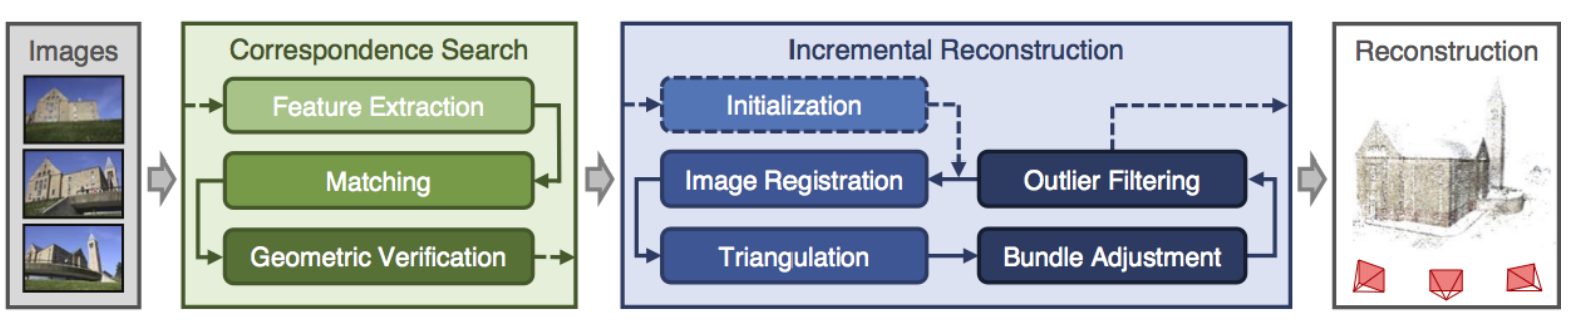
\includegraphics[width=0.8\textwidth]{images/COLMPA_pipeline.png}
    \caption{End-to-end SfM pipeline: feature extraction and matching, geometric verification, incremental camera/point estimation, and bundle adjustment.}
    \label{fig:sfm_pipeline_overview}
\end{figure}
SfM aims to recover both the 3D structure of a scene and the camera parameters that explain a set of images acquired from different viewpoints. In incremental pipelines such as COLMAP, this process is typically organized into the following stages:
\begin{enumerate}
    \item keypoint extraction;
    \item keypoint matching and geometric verification;
    \item incremental pose and sparse structure estimation;
    \item bundle adjustment refinement.
\end{enumerate}
The following exposition follows roughly this pipeline, from local features through two-view geometry, pose and triangulation, and finally bundle adjustment, with emphasis on geometric quantities that later become inputs to neural rendering methods.

\paragraph{Keypoint extraction (SIFT).}
The SfM pipeline starts from local visual evidence, and COLMAP commonly uses SIFT features \cite{lowe2004sift}. The scale-space representation is
\[
L(x,y,\sigma)=G(x,y,\sigma)\ast I(x,y),
\]
and keypoint candidates are selected as extrema of the Difference of Gaussians:
\[
D(x,y,\sigma)=L(x,y,k\sigma)-L(x,y,\sigma).
\]
SIFT then performs keypoint localization, orientation assignment, and descriptor computation. Each descriptor is a 128-dimensional vector.

\begin{figure}[H]
    \centering
    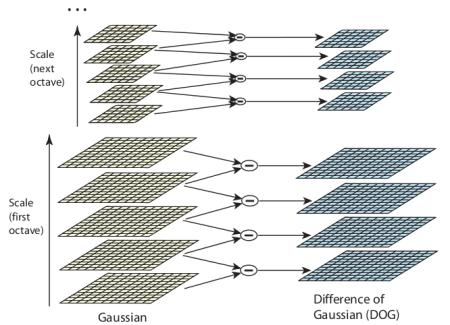
\includegraphics[width=0.5\textwidth]{images/sift_dog.jpg}
    \caption{Difference-of-Gaussians (DoG) used for scale-space extrema detection in SIFT.}
    \label{fig:sift_dog}
\end{figure}

The SIFT pipeline can be summarized in four steps:
\begin{itemize}
    \item \textbf{Scale-space extrema detection:} build $L$ and detect extrema of $D$.
    \item \textbf{Keypoint localization:} reject low-contrast candidates and unstable edge responses.
    \item \textbf{Orientation assignment:} estimate a dominant orientation from local gradients to achieve rotation invariance.
    \item \textbf{Descriptor computation:} aggregate gradient orientation histograms into a descriptor $d\in\mathbb{R}^{128}$.
\end{itemize}


These descriptors are designed to be robust to moderate illumination changes, scale changes, and rotations.

\paragraph{Descriptor matching.}
Once descriptors are extracted, the next step is to establish correspondences across views. Given images $I$ and $J$ with descriptor sets
\[
\mathcal{D}_I = \{d_I^1, \dots, d_I^{n_I}\}, \qquad
\mathcal{D}_J = \{d_J^1, \dots, d_J^{n_J}\},
\]
\begin{figure}[H]
    \centering
    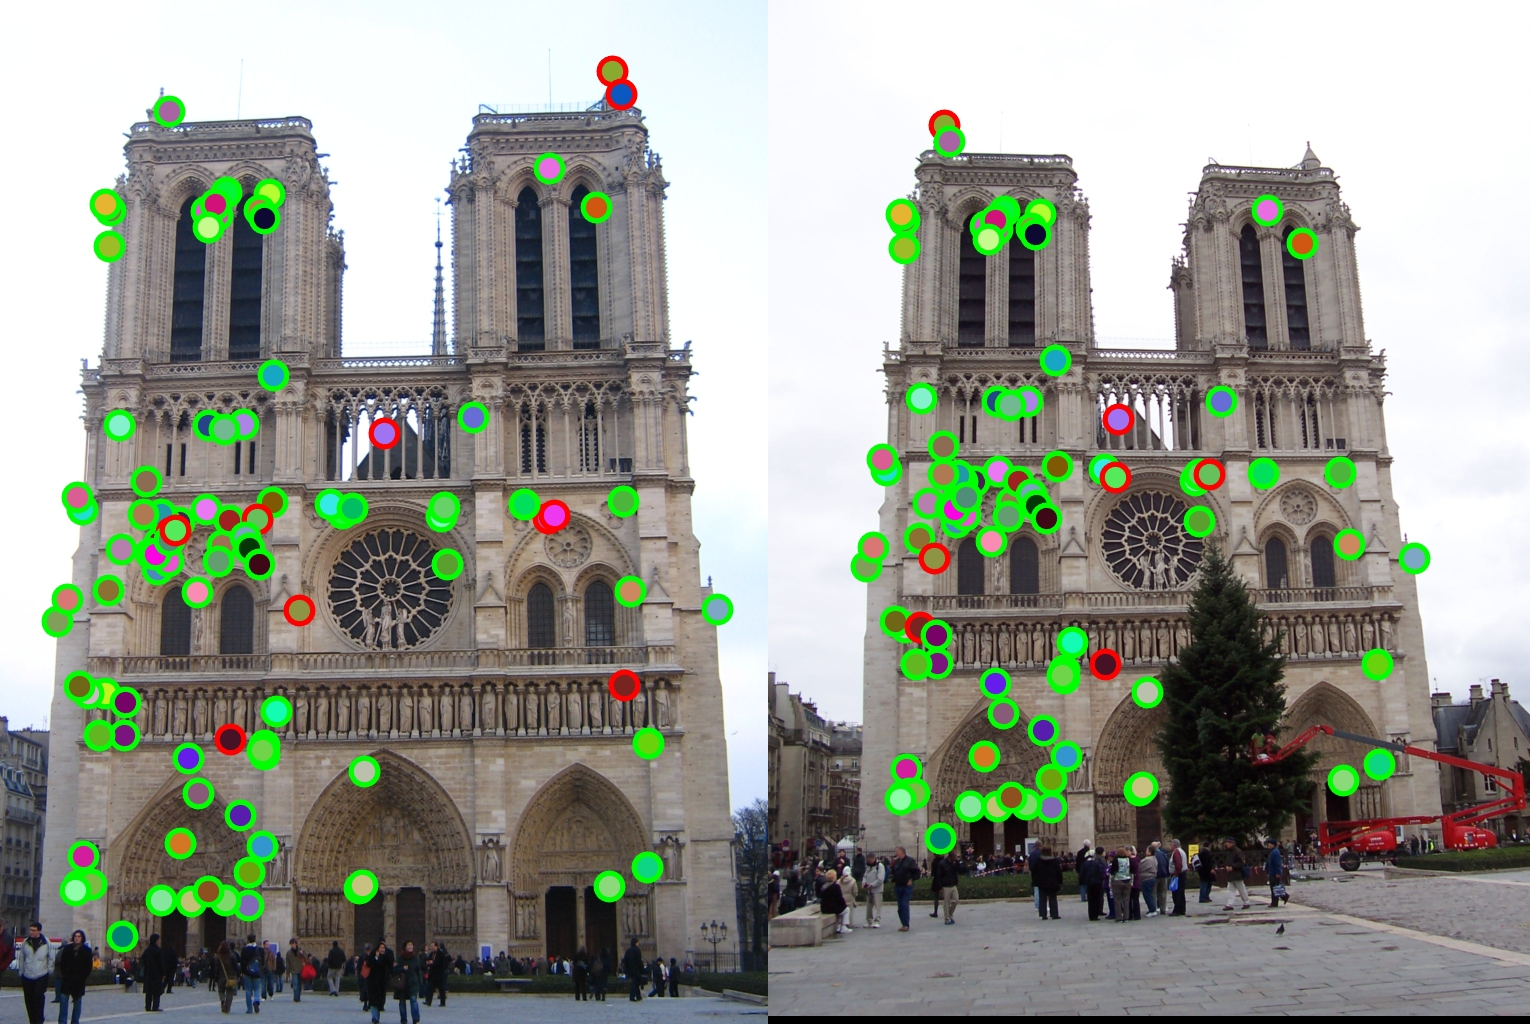
\includegraphics[width=0.3\textwidth]{images/keypoints_sift.jpg}
    \caption{SIFT keypoints detected over an image, before geometric matching across views.}
    \label{fig:sift_keypoints_only}
\end{figure}
matching is based on nearest-neighbor distance:
\[
\operatorname{dist}(d_i,d_j)=\|d_i-d_j\|_2.
\]
In practice, approximate nearest-neighbor search and Lowe's ratio test are applied for efficiency and robustness.

For a descriptor $d_I^m$ in image $I$, a nearest neighbor in image $J$ can be written as
\[
j^\star(m)=\arg\min_{p\in\{1,\dots,n_J\}} \left\|d_I^m-d_J^p\right\|_2.
\]
If the dataset contains $N$ images, naive exhaustive matching considers $\binom{N}{2}$ image pairs, which becomes expensive as $N$ grows. For this reason, practical systems restrict candidate pairs using scene overlap heuristics and accelerate nearest-neighbor search with libraries such as FLANN.

\begin{figure}[H]
    \centering
    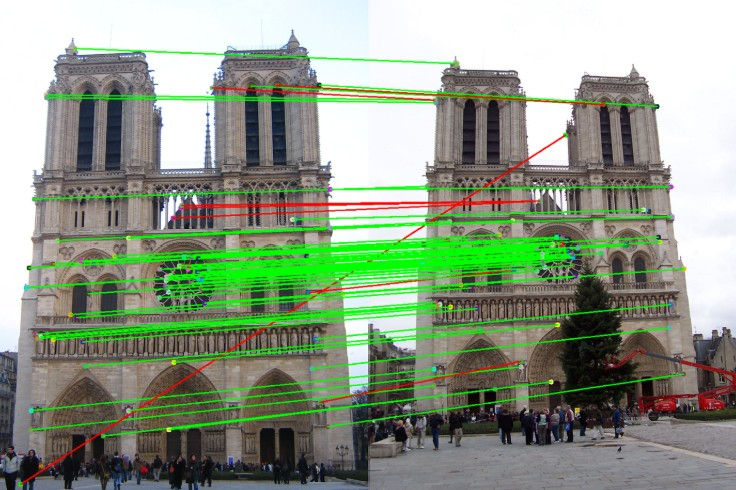
\includegraphics[width=0.3\textwidth]{images/matching_keypoints_SIFT.jpg}
    \caption{Example of SIFT keypoint correspondences between two views used for geometric verification and triangulation.}
    \label{fig:sift_keypoint_matching}
\end{figure}

\paragraph{Camera model and projection.}
After correspondences are defined in image space, camera projection links them to 3D geometry. A homogeneous 3D point $X=(X,Y,Z,1)^\top$ is projected to image point $x=(u,v,1)^\top$ via
\[
x \sim PX, \qquad P = K[R\mid t],
\]
with intrinsic matrix
\[
K=
\begin{bmatrix}
f_x & s & c_x \\
0 & f_y & c_y \\
0 & 0 & 1
\end{bmatrix}.
\]

\paragraph{SfM reconstruction and the observation graph.}
With this projection model in place, SfM estimates intrinsic parameters $K$, extrinsic parameters $(R,t)$ for each image, and a sparse set of 3D points $\{X_j\}$. 3D points are obtained by triangulation from multi-view correspondences. During incremental reconstruction, COLMAP maintains an \emph{observation graph} that links each 3D point to the images where it is observed. This graph is central for bundle adjustment because it defines which reprojection residuals are active for each parameter block.

In many COLMAP setups, all images from the same camera share a single intrinsic calibration $K$, while each image has its own pose $(R,t)$.

\paragraph{Epipolar geometry.}
Building on the previous matching and projection steps, epipolar geometry provides the key geometric link between image correspondences and relative camera pose: for corresponding points $x_1$ and $x_2$ in two views, the epipolar constraint is
\[
x_2^\top F x_1 = 0,
\]
where $F$ is the fundamental matrix (rank 2). With known intrinsics, the essential matrix is
\[
E = K^\top F K = [t]_\times R,
\]
with
\[
[t]_\times=
\begin{bmatrix}
0 & -t_z & t_y \\
t_z & 0 & -t_x \\
-t_y & t_x & 0
\end{bmatrix}.
\]

\begin{figure}[H]
    \centering
    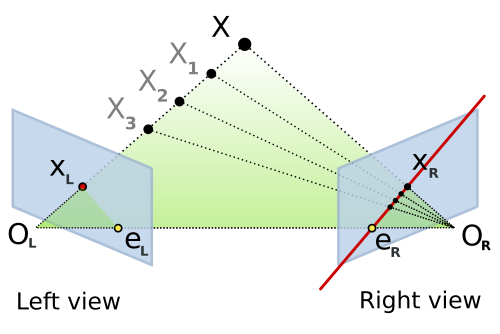
\includegraphics[width=0.3\textwidth]{images/Epipolar_geometry.svg.png}
    \caption{Two-view epipolar geometry with baseline, epipoles, and epipolar lines satisfying $x_2^\top F x_1=0$.}
    \label{fig:epipolar_geometry}
\end{figure}

The physically valid pose is selected with the cheirality condition after triangulation: the reconstructed points must be in front of the cameras.

Geometrically, epipolar geometry constrains correspondences: if $x_1$ is known in the first image, the match in the second image must lie on the epipolar line. In homogeneous coordinates, the epipolar line in the second image can be written as $l_2 \sim F x_1$. The epipole is the intersection of all epipolar lines in an image and corresponds to projecting the other camera center into the image plane.

\paragraph{Essential matrix (calibrated two-view geometry).}
To move from general two-view constraints to calibrated geometry, it is convenient to work in normalized image coordinates when intrinsic parameters are known:
\[
\hat{x} = K^{-1}x.
\]
In normalized coordinates, the epipolar constraint is expressed by the essential matrix $E$ as
\[
\hat{x}_2^\top E \hat{x}_1 = 0,
\qquad
E=[t]_\times R.
\]
The essential matrix has five degrees of freedom and, in the noise-free case, its singular values satisfy the characteristic constraint of a normalized essential matrix (two equal nonzero singular values and one zero singular value). With noisy measurements, a standard correction is to compute the SVD $E=U\Sigma V^\top$ and replace $\Sigma$ by a rank-2 matrix that enforces the essential-matrix singular-value pattern.

From $E$, one can recover up to four candidate motions $(R,t)$. The physically consistent solution is selected using cheirality after triangulating a set of points: the correct candidate maximizes the number of points with positive depth in both cameras.

\paragraph{Fundamental matrix estimation.}
Complementarily, for uncalibrated settings one works with the fundamental matrix, which encodes two-view geometry and has rank $2$. With at least eight point correspondences, one can formulate a linear system $Af=0$ where $f$ is a vectorization of $F$ and $A$ is built from the constraints $x_2^\top F x_1=0$. The minimal solution is obtained from the singular vector associated with the smallest singular value of $A$. Because noise breaks the rank constraint, a common post-processing step is to compute the SVD of the estimated matrix and set the smallest singular value to zero.

In practice, $F$ is commonly estimated with robust procedures such as the normalized 8-point algorithm embedded in RANSAC \cite{fischler1981ransac}. The linear system is solved up to scale and then projected to rank 2 by SVD. This step is essential because outlier correspondences from repeated textures, specularities, or dynamic objects can otherwise corrupt camera pose estimation.

\subsection{Camera Pose Estimation}
Building on these constraints, camera pose can be recovered from essential-matrix decomposition in calibrated two-view settings, or from Perspective-$n$-Point (PnP) when 2D--3D correspondences are available.

PnP is usually formulated as
\[
\min_{R,t} \sum_{k=1}^{n}\left\|\pi\!\left(K(RX_k+t)\right)-u_k\right\|_2^2.
\]
Incremental SfM typically alternates pose estimation, triangulation of new points, and local/global BA refinement.

From a geometric standpoint, two-view calibrated pose estimation from $E$ yields four candidate $(R,t)$ solutions. The correct one is chosen by enforcing positive depth (cheirality) for triangulated points in both cameras. This constraint is a key consistency check and removes physically invalid configurations.

\paragraph{PnP algorithms.}
Several specialized solvers exist for PnP, including minimal solvers (e.g., P3P) and efficient $n$-point formulations (e.g., EPnP). In incremental SfM, PnP is commonly used to register a new image once a sufficient set of 3D--2D correspondences is available from previously reconstructed structure.

\subsection{Sparse 3D Reconstruction}
Once camera poses are estimated, triangulation turns calibrated correspondences into 3D point coordinates. A linear estimate is usually computed first and then refined by nonlinear reprojection-error minimization.

\paragraph{Triangulation objective.}
For point observations across views, a common formulation is
\[
\min_{\tilde{X}} \sum_{j=1}^{M} \left\| \tilde{x}_j-\pi(P_j\tilde{X}) \right\|_2^2,
\]
where $\tilde{x}_j$ are measured image points, $P_j$ are known projection matrices for $M$ views, and $\tilde{X}$ is the unknown homogeneous 3D point.
This optimization is nonlinear due to perspective division; therefore, iterative solvers are used after linear initialization.

\paragraph{Linear initialization.}
A standard approach is the Direct Linear Transform (DLT) formulation, which rewrites each correspondence as linear constraints on $\tilde{X}$ and solves for $\tilde{X}$ in homogeneous coordinates up to scale. The linear estimate is subsequently refined by Gauss--Newton or Levenberg--Marquardt minimization of reprojection error.

When the baseline between views is too small, triangulation becomes ill-conditioned and depth uncertainty increases. For this reason, view selection and track quality have direct impact on reconstruction stability.

\paragraph{Bundle adjustment.}
After estimating camera poses and triangulating a sparse point cloud (possibly over several incremental steps), pipelines such as COLMAP tighten global consistency by minimizing reprojection error over all cameras and jointly over all tied 3D parameters. Let $\{C_i\}$ be camera parameters, $\{X_j\}$ 3D points, and $V_{ij}$ visibility. Bundle adjustment solves
\[
\min_{\{C_i\},\{X_j\}}
\sum_{i=1}^{I}\sum_{j=1}^{J}V_{ij}\,
\left\|
\pi(C_i, X_j)-x_{ij}
\right\|_2^2,
\]
where $\pi$ is projection into the image plane.

Bundle adjustment is a large sparse nonlinear least-squares problem. Modern SfM systems exploit the block-sparse structure of Jacobians and the Schur complement to optimize efficiently. This refinement is often the main factor behind the final metric quality of camera trajectories and sparse structure.

Bundle adjustment is a large sparse nonlinear least-squares problem. Modern SfM systems exploit the block-sparse structure of Jacobians and the Schur complement to optimize efficiently; implementations typically use sparse solvers (e.g.\ Ceres Solver) tailored to the sparsity pattern induced by the visibility structure. This refinement is often the main factor behind the final metric quality of camera trajectories and sparse structure.


\section{Neural Scene Representations}
\subsection{Neural Radiance Fields}
Having established the multi-view geometric background, we can now transition to neural scene representations. Before introducing NeRF, it is useful to recall the plenoptic function
\[
P(x,y,z,\theta,\phi,\lambda,t),
\]
which describes the intensity of light passing through a point in space along a direction, as a function of wavelength and time. A radiance field can be viewed as a simplified instance of this description, tailored to static scene reconstruction and rendering.

More formally, a radiance field maps position and viewing direction to emitted color and volume density:
\[
F(\mathbf{x},\mathbf{d}) \rightarrow (\mathbf{c},\sigma),
\]
where $\mathbf{x}\in\mathbb{R}^3$, $\mathbf{d}$ is a unit viewing direction, $\mathbf{c}$ is RGB color, and $\sigma$ is a nonnegative density that controls occlusion and transparency along rays.

Two broad families are commonly used to represent radiance fields:
\begin{enumerate}
    \item \textbf{Implicit representations}, where $F$ is implemented by a neural network, as in NeRF \cite{mildenhall2020nerf}.
    \item \textbf{Explicit representations}, where $F$ is stored using discrete structures such as voxel grids, point clouds, or collections of parametric primitives (including Gaussian-based methods).
\end{enumerate}

\paragraph{Neural Radiance Fields (NeRF).}
Starting from this formulation, NeRF \cite{mildenhall2020nerf} approximates the radiance field with an MLP $F_\Theta$:
\[
F_\Theta(\mathbf{x},\mathbf{d}) \rightarrow (\mathbf{c},\sigma),
\]
where $\Theta$ denotes learnable parameters. The scene geometry and appearance are therefore encoded implicitly in network weights rather than in an explicit mesh.

\begin{figure}[H]
    \centering
    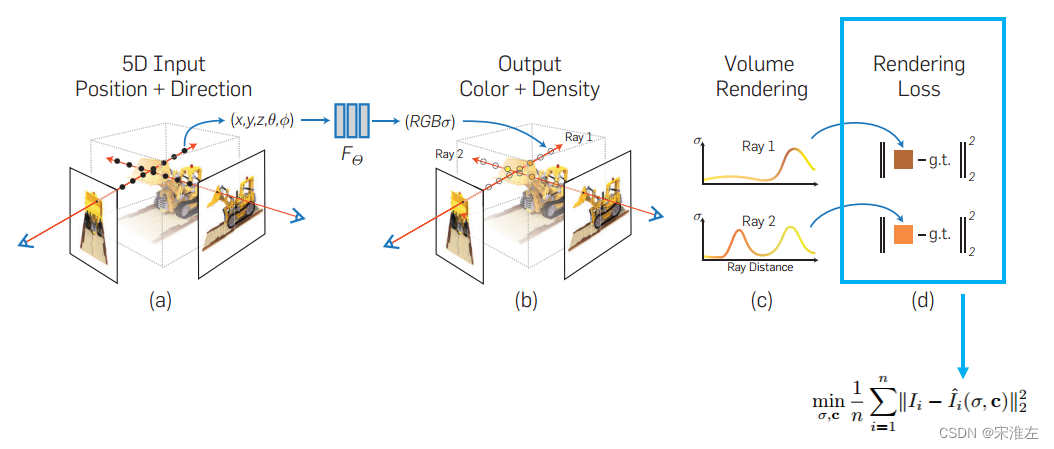
\includegraphics[width=0.8\textwidth]{images/NeRF.png}
    \caption{NeRF ray-based rendering: sample evaluation along rays and volumetric compositing of color and density.}
    \label{fig:nerf_ray_rendering}
\end{figure}

\paragraph{Ray casting and volume rendering.}
To connect the representation to image synthesis, NeRF renders by casting one ray per pixel from a given camera. A ray is parameterized by
\[
\mathbf{r}(t)=\mathbf{o}+t\mathbf{d},
\]
where $\mathbf{o}$ is the camera center and $\mathbf{d}$ is the ray direction.

NeRF does not intersect rays with explicit surfaces. Instead, it performs ray marching by sampling points $\{\mathbf{r}(t_i)\}_{i=1}^{N}$ between near and far bounds $(t_n,t_f)$. At each sample, the network predicts a color $\mathbf{c}_i$ and density $\sigma_i$. The predicted pixel color is obtained by the volume rendering integral
\[
C(\mathbf{r})=\int_{t_n}^{t_f} T(t)\,\sigma(\mathbf{r}(t))\,\mathbf{c}(\mathbf{r}(t),\mathbf{d})\,dt,
\]
with transmittance
\[
T(t)=\exp\!\left(-\int_{t_n}^{t}\sigma(\mathbf{r}(s))\,ds\right).
\]

\paragraph{Discrete approximation.}
For implementation, the continuous integral is approximated by a finite sum over ordered samples along the ray:
\[
\hat{C}(\mathbf{r})=\sum_{i=1}^{N}T_i\,\alpha_i\,\mathbf{c}_i,\quad
\alpha_i=1-\exp(-\sigma_i\delta_i),\quad
T_i=\prod_{j=1}^{i-1}(1-\alpha_j),
\]
where $\delta_i$ is the distance between consecutive samples. The term $\alpha_i$ can be interpreted as the probability that the ray terminates at sample $i$, while $T_i$ is the probability that the ray reaches sample $i$ without being absorbed earlier. This construction naturally models occlusion, semi-transparency, and view-dependent appearance when $\mathbf{c}_i$ depends on $\mathbf{d}$.

\paragraph{Training procedure.}
Given this rendering formulation, NeRF is trained from a set of images with known camera poses. For each sampled ray, the model renders $\hat{C}(\mathbf{r})$ and compares it to the ground-truth color $C_{\text{gt}}(\mathbf{r})$. A typical objective is mean squared error:
\[
\mathcal{L} = \sum_{\mathbf{r}}\left\|\hat{C}(\mathbf{r})-C_{\text{gt}}(\mathbf{r})\right\|_2^2.
\]


\subsection{3D Gaussian Splatting}
3D Gaussian Splatting (3DGS) represents a scene with explicit anisotropic Gaussian primitives optimized from calibrated views \cite{kerbl2023gaussian}. It combines high-quality rendering with real-time rasterization and builds on splatting principles connected to surface and EWA volume splatting \cite{zwicker2001surface,zwicker2002ewa}.

Similarly to NeRF, the goal is to reconstruct scene appearance from calibrated images and render novel viewpoints. However, the representation is fundamentally different: NeRF stores the radiance field implicitly in network weights, while 3DGS stores it explicitly as a collection of learnable volumetric primitives. Each Gaussian is defined by a position, an anisotropic shape, an opacity, and appearance parameters. In this sense, 3DGS still models density, color, visibility, and viewpoint, but without per-ray MLP queries.

This distinction matters for geometry: although optimized Gaussians often align with visible surfaces, they do not define a closed boundary mesh. Several primitives can overlap along the same viewing ray and still reduce photometric error without agreeing on a single depth, so the representation remains volumetric rather than a unique surface per object. 3DGS is therefore particularly strong for photorealistic novel view synthesis, while explicit geometry extraction remains challenging.

Compared to NeRF, 3DGS removes per-sample MLP evaluation along rays and instead projects explicit primitives directly to screen space. This architectural shift is central for real-time performance while preserving high rendering fidelity.

\begin{figure}[H]
    \centering
    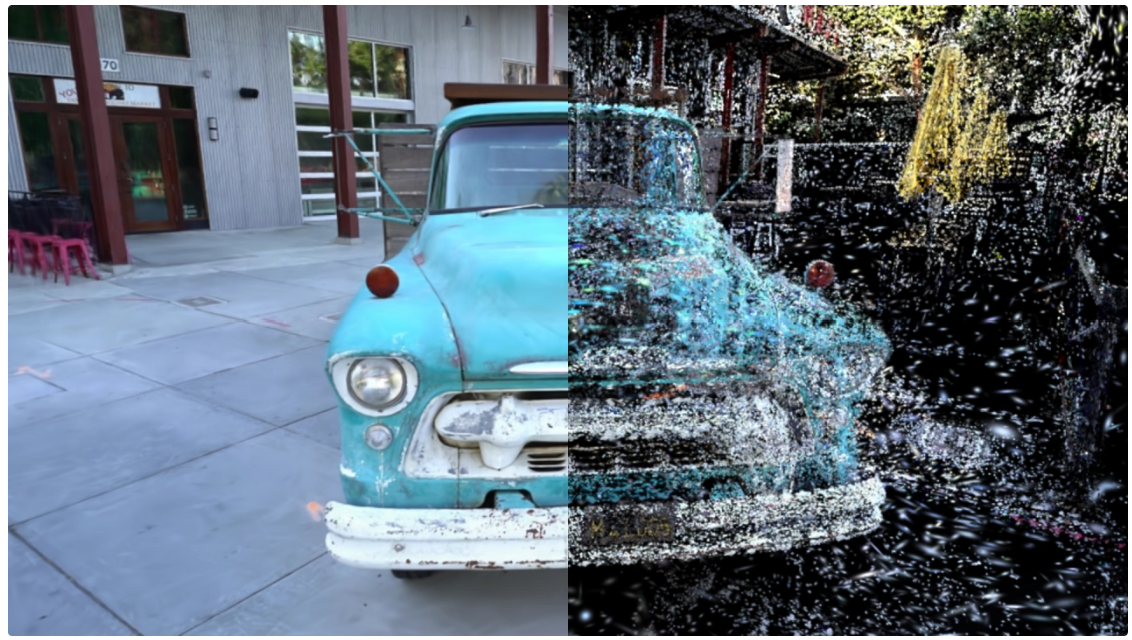
\includegraphics[width=0.5\textwidth]{images/result_3d_gaussian.png}
    \caption{Representative qualitative reconstruction/rendering result obtained with 3D Gaussian Splatting.}
    \label{fig:nerf_vs_3dgs}
\end{figure}

\subsubsection{Pipeline overview}
The full 3DGS pipeline can be summarized as:
\begin{enumerate}
    \item SfM-based data processing (camera calibration and sparse points);
    \item Gaussian initialization from sparse geometry;
    \item splatting-based rendering and alpha compositing;
    \item differentiable optimization of Gaussian parameters;
    \item adaptive density control (clone, split, prune);
    \item tile-based rasterization for efficient screen-space processing.
\end{enumerate}

\begin{figure}[H]
    \centering
    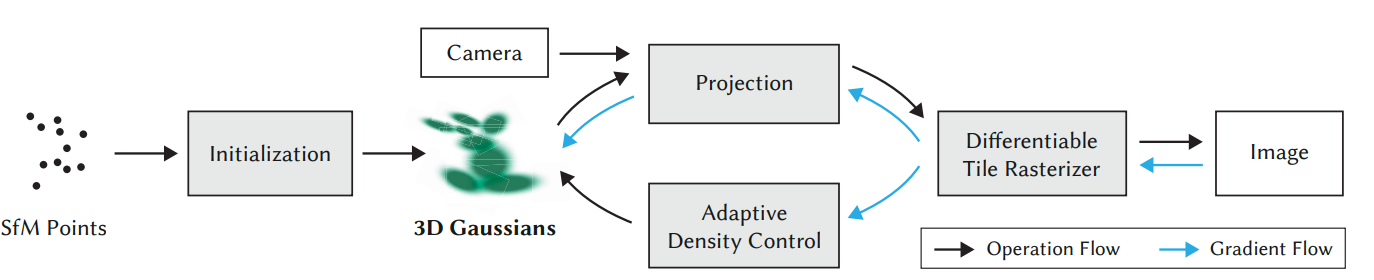
\includegraphics[width=0.7\textwidth]{images/full3dgaussiansplattinn.png}
    \caption{3DGS pipeline: SfM-based data processing, Gaussian initialization, splatting-based rendering and alpha compositing, differentiable optimization of Gaussian parameters, adaptive density control (clone, split, prune), tile-based rasterization for efficient screen-space processing.}
    \label{fig:3dgs_pipeline}
\end{figure}

\subsubsection{Relation with previous splatting methods}
Before detailing 3DGS, it is useful to recall the general idea of \emph{splatting}. In splatting, discrete primitives are projected to the image plane and accumulated into a continuous image. Each primitive defines a footprint in screen space and contributes to all pixels inside that footprint with weights given by a reconstruction kernel.

This is a forward-rendering viewpoint:
\begin{itemize}
    \item define primitives in world/object space;
    \item project them to screen space;
    \item compute a footprint region;
    \item accumulate weighted contributions into the framebuffer.
\end{itemize}
This differs from NeRF-style ray marching, where each pixel ray is traced independently through the volume.

\paragraph{Surface splatting.}
Surface splatting \cite{zwicker2001surface} renders surfaces represented by point samples without requiring an explicit triangle mesh. Each point is associated with a local surface element (\emph{surfel}) that projects to an elliptical footprint. From a signal-processing perspective, the rendered image can be understood as a weighted reconstruction of point attributes:
\[
f(\mathbf{x})=\sum_k w_k(\mathbf{x})\,f_k,
\]
where $f_k$ is an attribute (e.g., color) at sample $k$ and $w_k(\mathbf{x})$ depends on the distance between the pixel $\mathbf{x}$ and the projected footprint.

A central idea is Elliptical Weighted Average (EWA) filtering, which adapts the reconstruction kernel to anisotropic footprints induced by perspective projection. This reduces aliasing by combining reconstruction with a screen-space prefilter.

\begin{figure}[H]
    \centering
    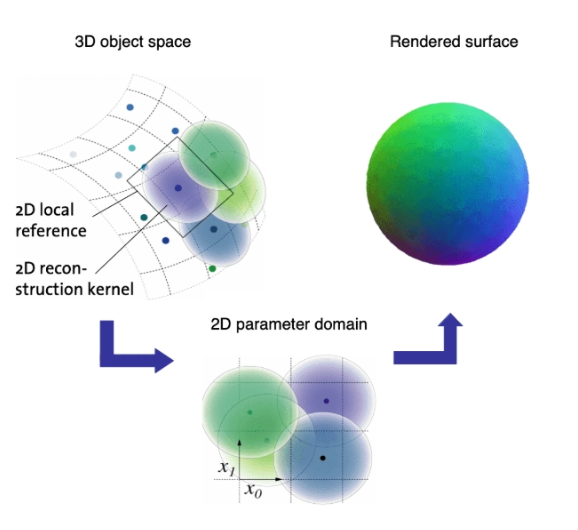
\includegraphics[width=0.5\textwidth]{images/surface_splatting.png}
    \caption{Surface splatting: each point is associated with a local surface element (surfel) that projects to an elliptical footprint.}
    \label{fig:surface_splatting}
\end{figure}

\paragraph{Volume splatting and EWA volume splatting.}
Volume splatting extends splatting to volumetric fields, closer to radiance-field rendering. In EWA volume splatting \cite{zwicker2002ewa}, volumetric primitives are often represented with Gaussian kernels. Gaussians are convenient because they are smooth, have easy derivatives for optimization, and admit convenient approximations under affine maps. In particular, a 3D Gaussian can be projected to a 2D footprint; intuitively, this can be interpreted as integrating a volumetric contribution along the viewing direction and representing its image-plane effect as an elliptical kernel.

The first stage of 3DGS estimates camera intrinsics and extrinsics and produces a sparse point cloud, typically using COLMAP \cite{schoenberger2016sfm,schoenberger2016mvs}. The objective is not to build a dense mesh, but to obtain a geometric prior suitable for initializing Gaussian means.

Let the sparse point cloud be
\[
\mathcal{P}=\{\mathbf{p}_i\}_{i=1}^{N},\qquad \mathbf{p}_i\in\mathbb{R}^3.
\]
A common initialization sets the Gaussian centers to SfM points,
\[
\boldsymbol{\mu}_i=\mathbf{p}_i.
\]
Camera poses are required at training time to project Gaussians into each training view and compare the rendered image to the observed image.

\subsubsection{Gaussian Parameterization}
Each primitive is parameterized by mean $\boldsymbol{\mu}_i$, covariance $\boldsymbol{\Sigma}_i$, opacity $o_i$, and view-dependent appearance coefficients (typically spherical harmonics).

\begin{figure}[H]
    \centering
    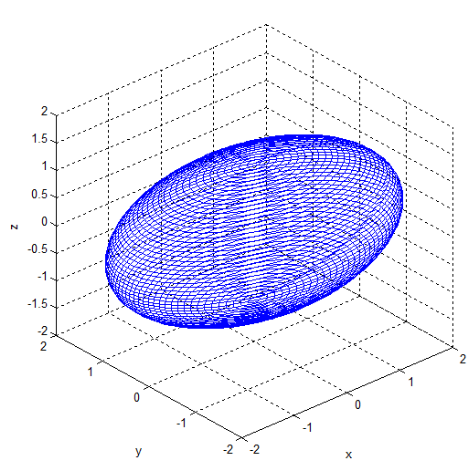
\includegraphics[width=0.35\textwidth]{images/3dGaussian.png}
    \caption{Single anisotropic 3D Gaussian primitive and its geometric parameters (center, covariance shape, and orientation).}
    \label{fig:gaussian_primitive_param}
\end{figure}

A typical Gaussian kernel is
\[
G_i(\mathbf{x})=\exp\!\left(-\frac{1}{2}(\mathbf{x}-\boldsymbol{\mu}_i)^\top
\boldsymbol{\Sigma}_i^{-1}(\mathbf{x}-\boldsymbol{\mu}_i)\right).
\]
To preserve valid covariance structure, $\boldsymbol{\Sigma}_i$ is parameterized through rotation and positive scales, e.g.
\[
\boldsymbol{\Sigma}_i=\mathbf{R}_i\mathbf{S}_i\mathbf{S}_i^\top\mathbf{R}_i^\top.
\]
In implementations, $\mathbf{R}_i$ is commonly represented by quaternions. Axis lengths are stored as \emph{log-scales} $\mathbf{s}_i\in\mathbb{R}^3$ and converted to $\boldsymbol{\sigma}_i=\exp(\mathbf{s}_i)$ before rasterization \cite{kerbl2023gaussian,tancik2023nerfstudio}: this enforces $\sigma>0$ without clipping under gradient descent and makes multiplicative shrink/grow steps more uniform when ellipsoid sizes span a wide range during densification.

The opacity $o_i$ modulates how strongly a Gaussian influences covered pixels. View-dependent color is represented by evaluating spherical harmonics as a function of viewing direction $\mathbf{d}$, denoted $\mathbf{c}_i(\mathbf{d})$.

\subsubsection{Splatting and rendering}
After initialization, rendering proceeds by splatting: each Gaussian is transformed to camera space, projected to the image plane, and rasterized as a 2D elliptical footprint. Unlike NeRF, 3DGS does not march rays through an implicit field; instead, it performs forward projection and accumulates contributions in image space.

At a high level, rendering executes the following steps:
\begin{enumerate}
    \item transform each Gaussian from world space to camera space;
    \item project the Gaussian center to the image plane;
    \item approximate the projected footprint as a 2D ellipse;
    \item evaluate the kernel response for pixels inside the footprint;
    \item composite contributions in depth order using alpha blending.
\end{enumerate}

\begin{figure}[H]
    \centering
    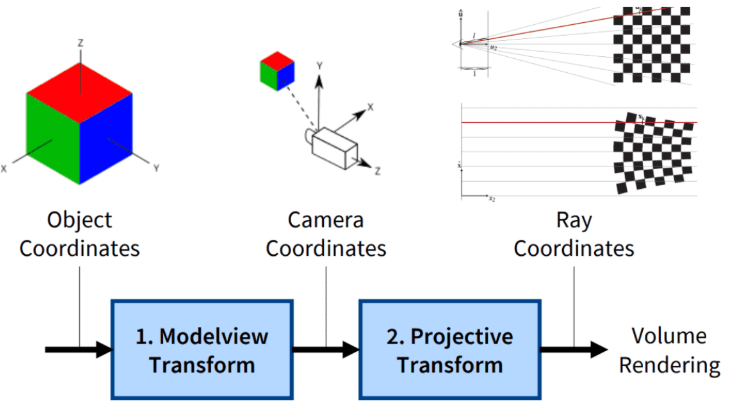
\includegraphics[width=0.5\textwidth]{images/complete_proiezioni.png}
    \caption{Multi-view projections involved in 3D Gaussian Splatting, relating camera observations to projected Gaussian structure.}
    \label{fig:multiview_projection_3dgs}
\end{figure}

\subsubsection{Transformation from world space to camera space}

Let $\boldsymbol{\mu} \in \mathbb{R}^3$ denote the Gaussian mean in world coordinates, with covariance $\boldsymbol{\Sigma} \in \mathbb{R}^{3 \times 3}$. Given the world-to-camera rotation $\mathbf{R}_{cw}$ and translation $\mathbf{t}_{cw}$, the mean in camera coordinates is

\[
\boldsymbol{\mu}_c = \mathbf{R}_{cw}\boldsymbol{\mu} + \mathbf{t}_{cw}.
\]

In homogeneous coordinates, this transformation can be written as

\[
\begin{bmatrix}
\boldsymbol{\mu}_c \\
1
\end{bmatrix}
=
\mathbf{T}_{cw}
\begin{bmatrix}
\boldsymbol{\mu} \\
1
\end{bmatrix},
\]

where $\mathbf{T}_{cw} \in \mathbb{R}^{4 \times 4}$ is the rigid transformation matrix.

The covariance transforms as

\[
\boldsymbol{\Sigma}_c = \mathbf{R}_{cw} \boldsymbol{\Sigma} \mathbf{R}_{cw}^\top,
\]

where the translation does not affect the covariance.

\subsubsection{Projection to ray space}

Following EWA volume splatting \cite{zwicker2002ewa}, \emph{ray space} is not the normalized image plane alone: it is a three-dimensional reparameterization of camera space in which the first two coordinates give the intersection of the viewing ray with the plane at unit depth ($z=1$), and the third records distance from the camera center along the ray. Let $\mathbf{x}_c=(x,y,z)^\top$ denote a point in camera coordinates (with $z>0$ in front of the camera). The mapping $g:\mathbb{R}^3\to\mathbb{R}^3$ is
\[
g(\mathbf{x}_c)=
\begin{pmatrix}
x/z \\[2pt]
y/z \\[2pt]
\|\mathbf{x}_c\|
\end{pmatrix},
\]
where $\|\mathbf{x}_c\|=\sqrt{x^2+y^2+z^2}$. The first two components coincide with \emph{normalized image coordinates} $(x/z,\,y/z)$; the third keeps a radial coordinate, so ray space remains $\mathbb{R}^3$ and should not be identified with image space $\mathbb{R}^2$.

The map $g$ is not affine. As in classical EWA splatting, one linearizes $g$ at the Gaussian mean $\boldsymbol{\mu}_c=(x,y,z)^\top$ using the Jacobian $\mathbf{J}\in\mathbb{R}^{3\times 3}$,
\[
\mathbf{J}=
\begin{pmatrix}
\frac{1}{z} & 0 & -\frac{x}{z^2} \\[4pt]
0 & \frac{1}{z} & -\frac{y}{z^2} \\[4pt]
\frac{x}{\|\mathbf{x}_c\|} & \frac{y}{\|\mathbf{x}_c\|} & \frac{z}{\|\mathbf{x}_c\|}
\end{pmatrix}_{\Big|\mathbf{x}_c=\boldsymbol{\mu}_c}.
\]
With $\boldsymbol{\Sigma}_c$ the camera-space covariance, a first-order propagated covariance in ray space is
\[
\boldsymbol{\Sigma}_{\mathrm{ray}} \approx \mathbf{J}\,\boldsymbol{\Sigma}_c\,\mathbf{J}^\top.
\]

\subsubsection{From ray space to the image-plane footprint}

Gaussians are closed under affine maps; under a fixed local linearization, the induced covariance remains quadratic in the tangent coordinates. The footprint used for splatting is a \emph{two-dimensional} Gaussian on the image plane (normalized coordinates). In the same local approximation, the marginal over the first two ray-space coordinates is obtained from the leading $2\times 2$ block of $\boldsymbol{\Sigma}_{\mathrm{ray}}$:
\[
\hat{\boldsymbol{\Sigma}} =
\begin{pmatrix}
[\boldsymbol{\Sigma}_{\mathrm{ray}}]_{11} & [\boldsymbol{\Sigma}_{\mathrm{ray}}]_{12} \\
[\boldsymbol{\Sigma}_{\mathrm{ray}}]_{21} & [\boldsymbol{\Sigma}_{\mathrm{ray}}]_{22}
\end{pmatrix},
\]
with mean in normalized coordinates $\boldsymbol{\mu}_{\mathrm{norm}}=(\mu_{c,1}/\mu_{c,3},\,\mu_{c,2}/\mu_{c,3})^\top$, i.e.\ the first two components of $g(\boldsymbol{\mu}_c)$. (Equivalently, one may motivate this reduction as integrating the 3D Gaussian contribution along the viewing direction in the EWA construction \cite{zwicker2002ewa}.)

\subsubsection{Projection to screen space}

Pixel coordinates apply the intrinsic matrix to homogeneous normalized coordinates. With
\[
\mathbf{K}=
\begin{pmatrix}
f_x & 0 & c_x \\
0 & f_y & c_y \\
0 & 0 & 1
\end{pmatrix},
\]
the projected mean is
\[
\boldsymbol{\mu}_{\mathrm{pix}}=
\begin{pmatrix}
f_x\,[\boldsymbol{\mu}_{\mathrm{norm}}]_1 + c_x \\
f_y\,[\boldsymbol{\mu}_{\mathrm{norm}}]_2 + c_y
\end{pmatrix}.
\]
For a diagonal scale from normalized to pixel coordinates (principal point handled in the mean), the screen-space covariance is
\[
\boldsymbol{\Sigma}_{\mathrm{pix}} \approx
\begin{pmatrix}
f_x & 0 \\
0 & f_y
\end{pmatrix}
\hat{\boldsymbol{\Sigma}}
\begin{pmatrix}
f_x & 0 \\
0 & f_y
\end{pmatrix}.
\]
Implementations often fold a single linearized map $\tilde{g}$ (normalized coordinates plus intrinsics in the first two components, distance in the third) and its $3\times 3$ Jacobian into one step before extracting the $2\times 2$ image block; the structure above matches that viewpoint while keeping the stages explicit.

The projected Gaussian footprint in screen space is
\[
g_i(\mathbf{x})=
\exp\!\left(
-\frac{1}{2}
(\mathbf{x}-\boldsymbol{\mu}_{\mathrm{pix},i})^\top
\boldsymbol{\Sigma}_{\mathrm{pix},i}^{-1}
(\mathbf{x}-\boldsymbol{\mu}_{\mathrm{pix},i})
\right),
\]
where $\mathbf{x}\in\mathbb{R}^2$ is a pixel coordinate.


\subsubsection{Rendering via Alpha Compositing}
At pixel $\mathbf{x}$, the opacity contribution of Gaussian $i$ combines learned opacity with the projected kernel:
\[
\alpha_i(\mathbf{x}) = o_i\,g_i(\mathbf{x}).
\]
Let Gaussians contributing to a pixel be sorted from front to back. The composited color is
\[
\mathbf{C}(\mathbf{x})=\sum_{i=1}^{N}T_i\,\alpha_i(\mathbf{x})\,\mathbf{c}_i(\mathbf{d}),\qquad
T_i=\prod_{j=1}^{i-1}\left(1-\alpha_j(\mathbf{x})\right),
\]
which mirrors alpha compositing used in volume rendering, but computed via rasterization of explicit primitives rather than ray integration through an MLP.

\begin{figure}[H]
    \centering
    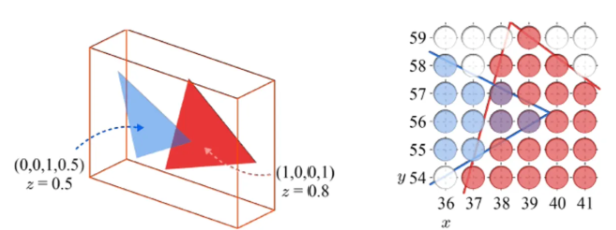
\includegraphics[width=0.5\textwidth]{images/alpha_blendig.png}
    \caption{Front-to-back alpha compositing intuition for accumulating Gaussian contributions along visibility order.}
    \label{fig:alpha_compositing_3dgs}
\end{figure}

\subsubsection{Photometric Optimization}
3DGS is trained with a photometric objective combining an $L_1$ term and a D-SSIM term:
\[
\mathcal{L}=(1-\lambda)\mathcal{L}_{1}+\lambda\mathcal{L}_{\text{D-SSIM}},
\qquad
\mathcal{L}_{\text{D-SSIM}}=\frac{1-\text{SSIM}(\hat{I},I)}{2},
\]
where $\hat{I}$ is the rendered image and $I$ is the ground truth for the sampled training view.

Let $\Theta=\{\boldsymbol{\mu}_i,\mathbf{s}_i,\mathbf{q}_i,o_i,\mathbf{c}_i\}_{i=1}^{N}$ denote all learnable parameters. Because rendering is differentiable, gradients $\nabla_\Theta \mathcal{L}$ can be computed and used in standard gradient-based optimizers:
\[
\Theta^{(t+1)}=\Theta^{(t)}-\eta \nabla_{\Theta}\mathcal{L}.
\]

\begin{algorithm}[htbp]
\caption{Optimization and Densification}
\label{alg:optimization_densification_3dgs}
\begin{algorithmic}[1]
\State \textbf{Input:} training image size $(w,h)$
\State $M \gets$ SfM points \Comment{initial Gaussian positions}
\State $S, C, A \gets \textsc{InitAttributes}()$ \Comment{covariances, colors, opacities}
\State $i \gets 0$
\While{not converged}
    \State $V, I_{\mathrm{gt}} \gets \textsc{SampleTrainingView}()$ \Comment{camera and image}
    \State $I \gets \textsc{Rasterize}(M,S,C,A,V)$ \Comment{see Algorithm~\ref{alg:rasterize_blending_3dgs}}
    \State $\mathcal{L} \gets \textsc{Loss}(I, I_{\mathrm{gt}})$
    \State $M,S,C,A \gets \textsc{AdamStep}(M,S,C,A,\nabla \mathcal{L})$
    \If{\textsc{IsRefinementIteration}($i$)}
        \For{all Gaussians $(\mu,\Sigma,c,\alpha)$}
            \If{$\alpha < \varepsilon$ \textbf{or} \textsc{TooLarge}($\mu,\Sigma$)}
                \State \textsc{RemoveGaussian}() \Comment{pruning}
            \EndIf
            \If{$\|\nabla_p \mathcal{L}\| > \tau_p$}
                \If{$\|\Sigma\| > \tau_s$}
                    \State \textsc{SplitGaussian}($\mu,\Sigma,c,\alpha$) \Comment{over-reconstruction}
                \Else
                    \State \textsc{CloneGaussian}($\mu,\Sigma,c,\alpha$) \Comment{under-reconstruction}
                \EndIf
            \EndIf
        \EndFor
    \EndIf
    \State $i \gets i + 1$
\EndWhile
\end{algorithmic}
\end{algorithm}

\subsubsection{Adaptive density control}
The initial SfM point cloud can be too sparse to represent fine details. 3DGS therefore modifies the set of primitives during training using \emph{adaptive density control}. Typical operations include:
\begin{itemize}
    \item \textbf{pruning} low-opacity or redundant Gaussians;
    \item \textbf{cloning} Gaussians in under-reconstructed regions;
    \item \textbf{splitting} large Gaussians into smaller ones when local detail is insufficient.
\end{itemize}
A common heuristic signal is the magnitude of the view-space positional gradient: large gradients often indicate that a Gaussian is important for explaining the image but is misaligned in position or scale.

\begin{figure}[H]
    \centering
    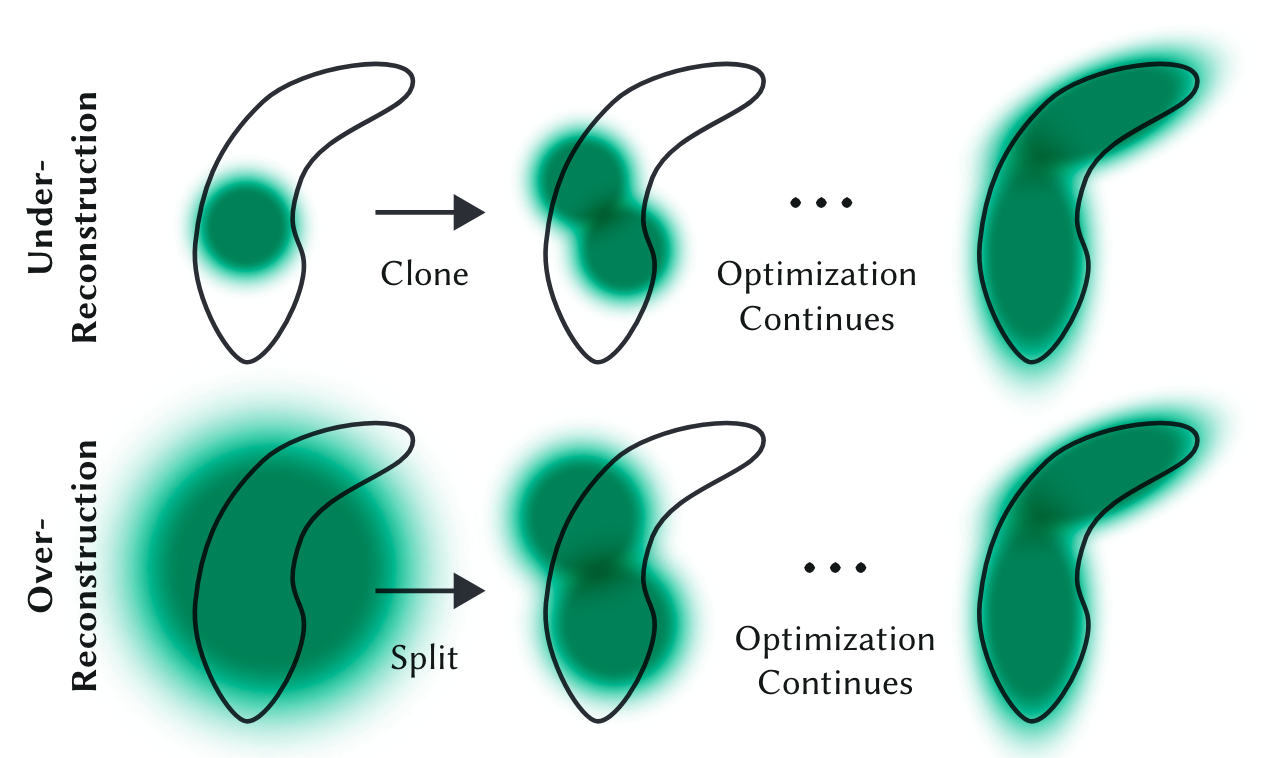
\includegraphics[width=0.5\textwidth]{images/adaptive_control_3Dgaussian.png}
    \caption{Adaptive density control in 3DGS (clone/split/prune) to improve coverage and local geometric detail.}
    \label{fig:3dgs_density_control}
\end{figure}

\subsubsection{Tile-based rasterization and visibility ordering}
Naively testing every Gaussian against every pixel is prohibitively expensive. Tile-based rasterization partitions the image into small tiles, assigns each Gaussian only to tiles intersected by its screen-space bounding box, sorts Gaussians by depth within each tile, and composites pixels using alpha blending.

\begin{figure}[H]
    \centering
    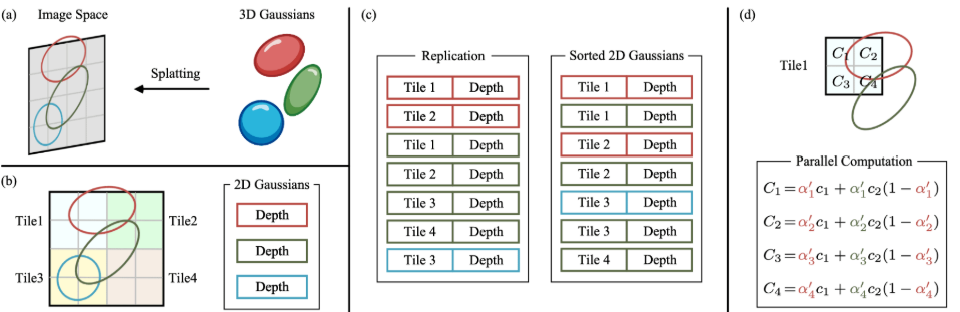
\includegraphics[width=0.7\textwidth]{images/complete_pipeline_3Dgaussian.png}
    \caption{3D Gaussian Splatting rendering flow: Gaussian parameterization, projection to screen-space ellipses, tile assignment, depth sorting, and compositing.}
    \label{fig:3dgs_projection_rasterization}
\end{figure}

\begin{algorithm}[htbp]
\caption{GPU Software Rasterization of 3D Gaussians}
\label{alg:rasterize_blending_3dgs}
\begin{algorithmic}[1]
\State \textbf{Input:} image size $(w,h)$, means $M$, covariances $S$, colors $C$, opacities $A$, view $V$
\State \textsc{CullGaussian}$(M,S,V)$ \Comment{frustum culling}
\State $M', S' \gets \textsc{ScreenspaceGaussians}(M,S,V)$ \Comment{transform}
\State $T \gets \textsc{CreateTiles}(w,h)$
\State $L,K \gets \textsc{DuplicateWithKeys}(M',T)$ \Comment{indices and keys}
\State \textsc{SortByKeys}$(K,L)$ \Comment{global sort}
\State $R \gets \textsc{IdentifyTileRanges}(T,K)$
\State $I \gets 0$ \Comment{initialize canvas}
\For{all tiles $t$ in $T$}
    \For{all pixels $i$ in $t$}
        \State $r \gets \textsc{GetTileRange}(R,t)$
        \State $I[i] \gets \textsc{BlendInOrder}(i,L,r,K,M',S',C,A)$
    \EndFor
\EndFor
\State \Return $I$
\end{algorithmic}
\end{algorithm}



\subsubsection{Limitations for Geometry Recovery}
Despite strong rendering quality, standard 3DGS still optimizes image consistency rather than explicit surface regularity. As a result, extracted geometry can be noisy, topologically ambiguous, or unstable in low-texture and occluded regions.

Moreover, thin structures and poorly observed regions can be represented by broad anisotropic blobs that explain color but do not correspond to physically plausible surfaces. This limitation motivates additional geometric supervision and structural priors, as developed in later chapters.

A practical manifestation of this behavior is the presence of \emph{floaters} (or floating Gaussians): small primitives that remain in incorrect 3D positions without matching a real surface (Figure~\ref{fig:floaters_example}). Training minimizes only the photometric loss $\mathcal{L}_{\mathrm{rgb}}$ (Section~2.3.5); for each Gaussian, position, scale, and opacity receive coupled gradients from that scalar objective through the rasterizer. If a misplaced primitive lowers $\mathcal{L}_{\mathrm{rgb}}$ on the training views where it is visible---for example by explaining residual color in poorly observed, reflective, or transparent regions---gradient descent has no incentive to remove it: its parameters sit at a \emph{local minimum} of $\mathcal{L}_{\mathrm{rgb}}$ (a stationary point of the loss landscape), meaning small joint changes to $(\boldsymbol{\mu},\mathbf{s},\alpha)$ would increase image error even though the 3D placement is wrong. Standard opacity-based pruning removes faint splats but does not penalize incorrect geometry directly; weak COLMAP initialization and subsequent densification can make such loss-minimizing yet geometrically invalid configurations more likely.

\begin{figure}[H]
    \centering
    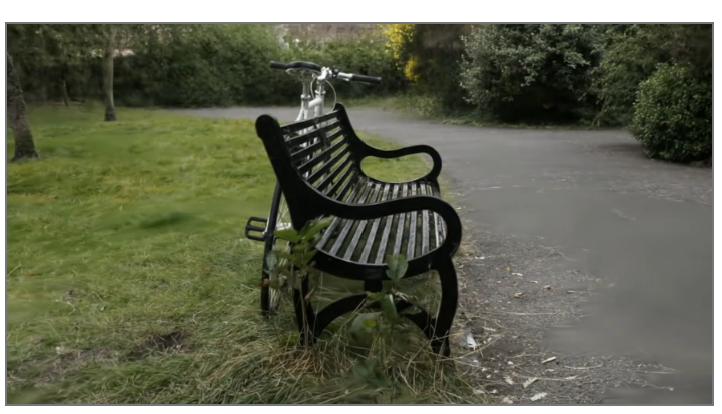
\includegraphics[width=0.35\textwidth]{images/floater_point.png}
    \caption{Example of floating Gaussians (floaters): primitives that reduce $\mathcal{L}_{\mathrm{rgb}}$ where they are seen but sit at geometrically invalid 3D locations.}
    \label{fig:floaters_example}
\end{figure}

\section{Depth in Neural Rendering}
To bridge appearance-driven rendering and geometry-aware optimization, this section focuses on the role of depth signals in neural rendering pipelines.

\subsection{Depth as Expected Value Along a Ray}
Neural radiance fields and many splatting-style renderers represent partially transparent media along viewing rays. As a consequence, a pixel does not correspond to a single surface intersection, but to an integral (or discrete sum) of contributions along the ray. Depth supervision must therefore specify \emph{which} notion of depth is being enforced.

\paragraph{Discrete volume rendering along a ray.}
Consider a camera ray through pixel $(x,y)$, with ordered samples indexed by $n=1,\dots,N$. Let $z_n$ denote the distance along the ray associated with sample $n$ (for example, the $z$ coordinate in camera space, or the Euclidean distance from the camera center, depending on implementation). Let $\alpha_n\in[0,1]$ denote the opacity (or occupancy) predicted at sample $n$, and let $T_n$ denote the transmittance up to sample $n$, i.e., the probability that the ray reaches sample $n$ without being fully stopped by earlier material.

Under the standard NeRF-style alpha compositing model, one defines
\[
T_1=1,\qquad
T_n=\prod_{k=1}^{n-1}(1-\alpha_k),\quad n>1,
\]
and the compositing weight for sample $n$ is $w_n=\alpha_n T_n$.

\paragraph{Accumulated depth vs.\ expected depth.}
With compositing weights defined, two common scalar summaries of ray depth are the \emph{accumulated depth} and the \emph{expected depth}. They can be written as
\begin{equation}
d_{x,y}^{\mathrm{acc}}=\sum_{n=1}^{N} z_n\,\alpha_n\,T_n,
\label{eq:depth_accumulated}
\end{equation}
and
\begin{equation}
d_{x,y}^{\mathrm{exp}}=
\frac{\sum_{n=1}^{N} z_n\,\alpha_n\,T_n}{\sum_{n=1}^{N} \alpha_n\,T_n}
=
\frac{d_{x,y}^{\mathrm{acc}}}{\sum_{n=1}^{N} w_n}.
\label{eq:depth_expected}
\end{equation}
Equation~\eqref{eq:depth_accumulated} aggregates depth contributions weighted by how much each sample affects the final pixel color. Equation~\eqref{eq:depth_expected} normalizes the same numerator by the total mass $\sum_n w_n$, producing a weighted average depth along the ray.

\paragraph{Relationship to compositing weights.}
From these definitions, and since $w_n=\alpha_n T_n$, the expected depth can equivalently be expressed as
\[
d_{x,y}^{\mathrm{exp}}=\sum_{n=1}^{N} \tilde{w}_n\, z_n,
\qquad
\tilde{w}_n=\frac{w_n}{\sum_{k=1}^{N} w_k},
\]
whenever $\sum_k w_k>0$. If $\sum_k w_k$ is substantially smaller than $1$, a large portion of the ray remains ``free space''; in that regime, depth summaries become sensitive to how ``empty space'' is handled numerically (epsilon stabilization, background models, or sky handling).

\paragraph{Semantic differences and failure modes.}
At this point it is useful to clarify interpretation: accumulated depth and expected depth answer different questions. The accumulated quantity grows with both geometry and visibility mass; the expected depth isolates a \emph{mean} depth under the induced distribution $\tilde{w}_n$. Both are fragile in qualitatively difficult cases:
\begin{itemize}
    \item \textbf{Multi-modality along a ray:} semi-transparent surfaces, foliage, fences, or motion blur can create multiple separated modes in $w_n$. Any single scalar depth collapses this structure and can be unstable under small changes in $\alpha_n$.
    \item \textbf{View dependence:} if opacity is view-dependent, depth summaries can change between cameras even for a fixed world point, which is problematic when enforcing multi-view consistency.
    \item \textbf{Scale alignment:} monocular depth priors are often defined up to unknown scale (and sometimes shift). Comparing $d^{\mathrm{exp}}$ to such priors therefore requires explicit alignment per image or per scene.
\end{itemize}

\subsection{Monocular Metric Depth Estimation}
To complement renderer-internal depth definitions, monocular depth estimation aims to predict a dense depth map from a single RGB image. In robotics and metrology, one often desires \emph{metric} depth in real-world units. However, many high-performing monocular models are trained to predict \emph{relative} depth up to an unknown affine ambiguity (scale and possibly shift), because diverse training domains do not share a single consistent metric scale.

\paragraph{From relative predictions to metric depth.}
In practical pipelines, metric depth is recovered by combining a relative-depth network with additional information, for example:
\begin{itemize}
    \item \textbf{Calibration and ground control:} known baselines, object sizes, or sparse LiDAR measurements to fix scale/shift.
    \item \textbf{Multi-view constraints:} epipolar geometry couples depths across views, which can reduce scale drift when cameras are calibrated.
    \item \textbf{Domain-specific fine-tuning:} supervised fine-tuning on datasets with metric ground truth (e.g., indoor RGB-D or automotive datasets).
\end{itemize}

\subsection{Depth Anything v3}
As a concrete model family aligned with these needs, Depth Anything 3 (DA3) is a general-purpose visual geometry model that predicts spatially consistent geometry from an arbitrary number of inputs (a single image, multi-view batches, or video), with or without known camera poses \cite{lin2025depthanything3}. The stated design goal is \emph{minimal modeling}: a plain pretrained vision transformer backbone (e.g., DINOv2) without bespoke geometric modules, trained to predict a compact set of dense outputs that still encode enough information to recover camera motion and scene structure.

\paragraph{Positioning relative to Depth Anything 1--2.}
Depth Anything (DA1) established a strong monocular foundation model by scaling dataset diversity and using large-scale training strategies that combine labeled and unlabeled data \cite{yang2024depth}. Depth Anything V2 (DA2) refined robustness and detail, producing monocular relative-depth models widely used as priors in 3D pipelines \cite{yang2024depthanythingv2}.

DA3 marks a generational shift in the series: it expands the operating regime from ``single image in, single depth map out'' to \emph{any-view} inference, jointly reasoning about multiple images and producing outputs that support consistent fusion into point clouds and downstream 3D representations \cite{lin2025depthanything3}. In monocular mode, DA3 is reported to surpass DA2 while preserving strong detail and robustness \cite{lin2025depthanything3}.

\paragraph{Core outputs: depth maps and ray maps.}
Given $N_v$ input images $\{\mathbf{I}_i\}_{i=1}^{N_v}$, DA3 produces per-view dense depth maps $\mathbf{D}_i$ aligned with pixels, and additionally predicts dense \emph{ray maps} that represent camera rays in a form that can be fused with depth to recover 3D points without directly regressing a rotation matrix with hard orthogonality constraints \cite{lin2025depthanything3}. Intuitively, predicting rays together with depths is a way to unify pose and geometry in a single feed-forward framework: depth explains ``how far along the ray'', while the ray field explains ``which ray belongs to each pixel in a global frame''.

\paragraph{Architecture (what is minimal and what is not).}
DA3 uses a ViT backbone and introduces an \emph{input-adaptive} cross-view self-attention mechanism implemented by reordering tokens in selected transformer blocks, enabling cross-image information exchange without changing the backbone architecture class \cite{lin2025depthanything3}. A dual DPT-style decoder head then predicts depth and ray maps from shared intermediate features, using separate fusion branches so the two tasks interact while avoiding redundant intermediate representations \cite{lin2025depthanything3}.

When camera intrinsics/extrinsics are known, DA3 can encode them as additional tokens that participate in attention; when unknown, a learnable camera token provides a consistent placeholder so the same model can operate in both posed and pose-free settings \cite{lin2025depthanything3}.

\begin{figure}[H]
    \centering
    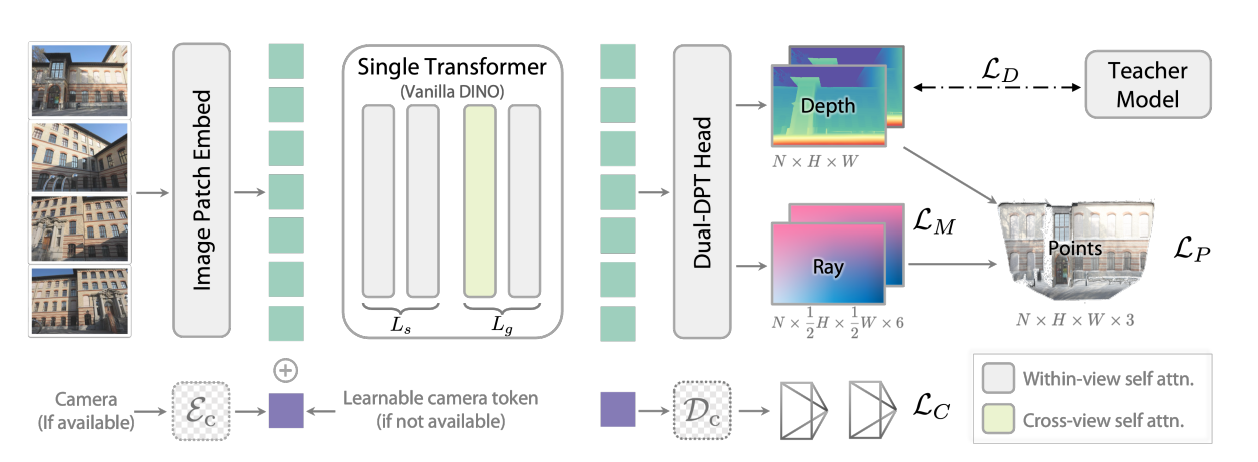
\includegraphics[width=0.8\textwidth]{images/pipelinedv3.png}
    \caption{Depth Anything 3 architecture (adapted from \cite{lin2025depthanything3}). $N$ input views are patch-embedded and processed by a DINO transformer with alternating within-view ($L_s$) and cross-view ($L_g$) self-attention. A dual-DPT head predicts per-view depth and ray maps; depth is supervised against a teacher model ($\mathcal{L}_D$), while ray maps and lifted 3D points are trained with $\mathcal{L}_M$ and $\mathcal{L}_P$. When camera parameters are unknown, a learnable camera token feeds an optional pose decoder ($\mathcal{L}_C$).}
    \label{fig:da3_pipeline}
\end{figure}

\paragraph{Training as teacher--student with pseudo-depth alignment (padre--figlio).}
DA3 is trained on heterogeneous supervision sources (synthetic renders, reconstructions, and real captures). Real-world depth supervision is often sparse, incomplete, or noisy; training directly on such labels can limit fine detail \cite{lin2025depthanything3}. DA3 therefore adopts a teacher--student paradigm closely inspired by prior Depth Anything pseudo-labeling ideas \cite{yang2024depth,yang2024depthanythingv2}:
\begin{itemize}
    \item \textbf{Teacher (padre):} a strong monocular relative-depth model trained on large synthetic data to produce dense pseudo-depth with high-frequency detail.
    \item \textbf{Student (figlio):} the DA3 model trained to match pseudo labels while remaining anchored to original sparse/noisy ground truth.
\end{itemize}
Crucially, the teacher pseudo-depth is aligned to the available real measurements using robust scale/shift fitting (the paper specifies RANSAC least squares), intended to preserve global geometric fidelity while gaining dense completeness \cite{lin2025depthanything3}. The DA3 teacher extends DA2-style training along two axes emphasized in the paper: \emph{data scaling} on a substantially expanded synthetic corpus, and a revised \emph{depth representation} (predicting scale--shift invariant depth rather than disparity, and using an exponential parameterization of depth to improve near-range sensitivity) \cite{yang2024depthanythingv2,lin2025depthanything3}; its objective combines multiple geometric signals (including gradient supervision and additional normal-based terms described in the paper) to improve local planarity and edge behavior for downstream 3D use \cite{lin2025depthanything3}. The student is trained with a composite objective that supervises predicted depth and ray maps, encourages predicted point maps to agree with supervision, includes an optional camera prediction term when poses are used, and uses a depth-gradient loss to preserve sharp discontinuities while maintaining smooth planar regions \cite{lin2025depthanything3}. The paper also describes a training schedule where supervision transitions from ground-truth signals to teacher pseudo-labels during training, which operationalizes the idea that early training should respect metric/sparse constraints, while later training can safely densify detail \cite{lin2025depthanything3}.

\paragraph{Implementation-scale training details (why DA3 is not ``just a bigger DA2'').}
The paper reports large-scale training on many public datasets spanning synthetic, LiDAR, and reconstruction-derived labels, with a long schedule on modern accelerators and a deliberately chosen base resolution grid designed to be compatible with common aspect ratios \cite{lin2025depthanything3}. Beyond dataset scale, two training mechanisms are particularly important for thesis readers:
\begin{itemize}
    \item \textbf{Curriculum from clean constraints to dense pseudo labels:} switching supervision sources during training reduces the risk that dense-but-imperfect pseudo depth overwhelms early optimization before the model has learned coarse geometric consistency \cite{lin2025depthanything3}.
    \item \textbf{Randomized pose conditioning:} occasionally providing ground-truth intrinsics/extrinsics during training teaches the model to exploit pose cues when available, while still remaining usable when poses are unknown at inference time \cite{lin2025depthanything3}.
\end{itemize}



\paragraph{Use in this thesis.}
In the Splatfacto implementation developed for this thesis, DA3 is used only as a \emph{monocular} depth prior: for each training view, a dense depth target is computed independently from the ground-truth RGB image. The checkpoint \textbf{DA3METRIC-LARGE} (\emph{Monocular Metric Depth}) is used rather than a relative-depth variant; its output is converted to metric depth in meters using the known focal length in pixels, so no per-image affine scale--shift alignment is required when supervising rendered depth in camera space. Poses and intrinsics are taken from COLMAP, not from DA3; the multi-view cross-attention, ray maps, and optional camera head of the full DA3 framework are outside the scope of this work.



\section{Surface-Based Representations}
After depth priors, the discussion shifts to explicit parametric geometry used in this thesis to improve structural control.

\subsection{B\'ezier Curves and Surfaces}
This section reviews B\'ezier curves and tensor-product B\'ezier surfaces as explicit parametric geometry. The definitions below underpin the surface-based modifications developed in Chapter~\ref{chap:methodology}: B\'ezier models offer a compact set of control parameters that induce smooth geometry and support stable optimization under image-based supervision.

\paragraph{Bernstein basis and B\'ezier curves.}
A degree-$M$ B\'ezier curve is a polynomial curve in $\mathbb{R}^d$ parameterized by $t\in[0,1]$:
\[
\mathbf{B}(t)=\sum_{j=0}^{M} B_j^{M}(t)\,\mathbf{p}_j,
\qquad
B_j^{M}(t)=\binom{M}{j}(1-t)^{M-j}t^{j},
\]
where $\{\mathbf{p}_j\}_{j=0}^{M}$ are control points. The basis functions $B_j^{M}$ are nonnegative on $[0,1]$ and partition unity, $\sum_j B_j^{M}(t)=1$. Consequently, $\mathbf{B}(t)$ lies in the convex hull of the control polygon for all $t\in[0,1]$ (convex-hull property), which is useful as a geometric prior: feasible shapes are globally constrained by a small number of control points.

\begin{figure}[H]
    \centering
    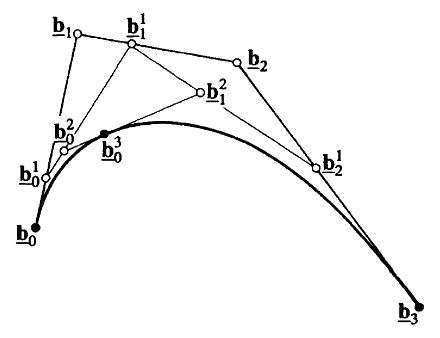
\includegraphics[width=0.5\textwidth]{images/curve_di_bezier.png}
    \caption{B\'ezier curve example with control polygon and resulting smooth trajectory, illustrating Bernstein interpolation and convex-hull behavior.}
    \label{fig:bezier_curve_example}
\end{figure}

\paragraph{Geometric meaning of control points.}
From this basis representation, the geometric role of control points becomes clearer. Increasing the degree increases expressivity at the cost of more parameters and potential oscillation (Runge-type phenomena) if control points are poorly placed. In practice, complex shapes are represented by joining multiple B\'ezier segments with continuity constraints at junctions. B\'ezier curves are differentiable polynomials; the tangent direction follows from differentiating the Bernstein expansion. For optimization, this matters because objective functions that depend on positions on the curve (e.g., through rendering) can backpropagate gradients to control points through the chain rule, provided downstream operations are differentiable.

\paragraph{Tensor-product B\'ezier surfaces.}
Extending the same idea from curves to surfaces, a tensor-product B\'ezier patch maps parameters $(u,v)\in[0,1]^2$ into $\mathbb{R}^3$ by separating variation along $u$ and $v$:
\[
\mathbf{S}(u,v)=\sum_{i=0}^{M_u}\sum_{j=0}^{M_v}
B_i^{M_u}(u)\,B_j^{M_v}(v)\,\mathbf{p}_{i,j},
\]
where $\{\mathbf{p}_{i,j}\}$ form a rectangular control net. Intuitively, each iso-$v$ curve is a B\'ezier curve in $u$, and each iso-$u$ curve is a B\'ezier curve in $v$. This separability is convenient for sampling, texturing, and enforcing regularity: smoothness in $u$ and $v$ is inherited from the smoothness of Bernstein polynomials.

\begin{figure}[H]
    \centering
    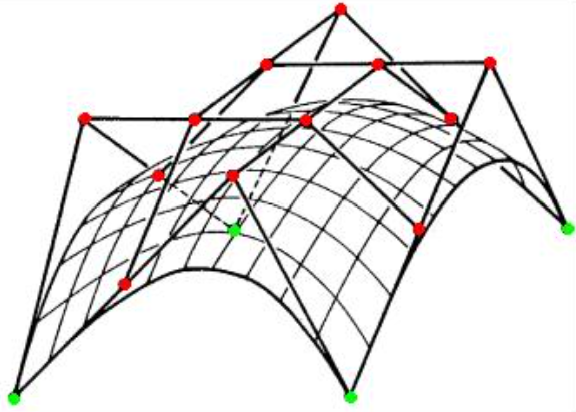
\includegraphics[width=0.5\textwidth]{images/surface_bezier.png}
    \caption{Tensor-product B\'ezier surface with control net: variation along $(u,v)$ generates a smooth parametric patch in $\mathbb{R}^3$.}
    \label{fig:bezier_surface_example}
\end{figure}

\paragraph{Local shape control and continuity across patches.}
Moving one control point $\mathbf{p}_{i,j}$ influences the surface locally, with influence strongest near the corresponding parameter region but generally nonzero across the patch (global support of Bernstein basis on $[0,1]^2$). Complex objects are therefore often modeled by multiple patches with $C^0$, $C^1$, or higher continuity enforced along shared boundaries by constraining control nets (e.g., colinearity of adjacent control edges for $C^1$ transitions).

\subsection{B\'ezier-Based Splatting Approaches}
To connect these geometric primitives with rendering practice, recent work on \emph{B\'ezier Splatting} studies how to combine parametric B\'ezier primitives with Gaussian splatting-style rasterization for differentiable vector graphics \cite{liu2025bezier}. The central theoretical idea is to replace exact boundary-centric rasterization of curves (as in classical differentiable vector renderers) with an explicit, kernel-based accumulation of Gaussians placed along, and in the vicinity of, B\'ezier curves, exploiting the fact that Gaussian footprints yield stable spatial gradients in image space while remaining compatible with fast tile-based rasterization \cite{liu2025bezier,kerbl2023gaussian}.

\paragraph{From curves in 2D to surfaces in 3D (conceptual lift).}
In vector graphics, B\'ezier curves live in $\mathbb{R}^2$ and partition the image into stroke and non-stroke regions. In 3D scene reconstruction, one may analogously treat a B\'ezier \emph{surface} $\mathbf{S}(u,v)\subset\mathbb{R}^3$ as a low-dimensional geometric scaffold that explains a subset of the scene (typically an object-centric region). The same structural principle applies:
\begin{itemize}
    \item \textbf{Explicit parameterization:} geometry is controlled by a control net rather than by unconstrained point clouds.
    \item \textbf{Differentiable sampling:} points $\mathbf{S}(u,v)$ (and local frames induced by partial derivatives $\partial_u \mathbf{S}$, $\partial_v \mathbf{S}$) can be used as anchors for volumetric primitives.
    \item \textbf{Splatting viewpoint:} rendering can be understood as projecting localized kernels to the image plane and compositing contributions, rather than solving hard boundary predicates per pixel.
\end{itemize}

\paragraph{How this thesis uses surfaces ``like curves'' at a high level.}
At the level of theory (not implementation), the methodological analogy is:
\begin{enumerate}
    \item define an explicit B\'ezier \emph{surface patch} that approximates visible object geometry in 3D;
    \item generate a structured set of 3D locations on (and optionally near) the patch by sampling $(u,v)$ and optional offsets along a local normal direction;
    \item associate each location with a localized volumetric primitive whose parameters are tied to the patch (positionally anchored, with anisotropy aligned to local tangents);
    \item optimize patch parameters jointly with the rendering objective, so image residuals update the control net through the sampled primitive chain.
\end{enumerate}
This mirrors the 2D B\'ezier splatting philosophy, ``optimize parametric geometry through splatted kernels'', while replacing curve arclength by surface parameters $(u,v)$ and replacing planar strokes by embedded surfaces in $\mathbb{R}^3$ \cite{liu2025bezier}.

\paragraph{Pruning/densification as a geometric analogue.}
B\'ezier Splatting emphasizes adaptive allocation of curve capacity: remove negligible primitives and densify where reconstruction error remains high, interpreting densification as enlarging the effective receptive field of the parametric model \cite{liu2025bezier}. The same conceptual mechanism carries over to surfaces: patch refinement can be viewed as reallocating representational budget where photometric gradients indicate persistent mismatch between rendered and observed images.

\section{Semantic Object Segmentation}
To support object-centric initialization, many 3D reconstruction pipelines need to isolate a subset of geometry and appearance that corresponds to a user-specified entity. In this thesis, semantic isolation is obtained by combining \emph{text-conditioned localization} with \emph{promptable segmentation}:
\begin{itemize}
    \item Grounding DINO proposes boxes (and associated language alignments) from free-form text \cite{liu2023groundingdino}.
    \item SAM~2 turns boxes/clicks/masks into high-quality region masks and can propagate them across views or time \cite{ravi2024sam2}.
\end{itemize}
The following subsections summarize the underlying models at the same level of technical depth used for depth foundation models elsewhere in this chapter.

\subsection{GroundingDINO}
In multi-view pipelines, text prompts can be applied independently per image (or on a reference view) to obtain candidate boxes. These boxes define image regions whose corresponding rays and sparse points can be aggregated into an object-centric working set. Grounding DINO is an open-set object detector that accepts a free-text prompt and predicts a set of bounding boxes aligned with noun phrases in the text \cite{liu2023groundingdino}. The motivating problem is \emph{open-set} (or open-vocabulary) detection: the model must generalize beyond a fixed category list by grounding visual regions in language, rather than classifying into a closed label space \cite{liu2023groundingdino}.

\paragraph{From closed-set detection to language-grounded detection.}
Classical detectors map each region embedding to one of $K$ training categories. Open-set detectors instead seek a joint embedding space where a region can be matched to arbitrary text tokens (words or phrases). Grounding DINO follows the GLIP-style perspective that object detection can be formulated as phrase grounding at scale, but requires language to be fused throughout the pipeline rather than at a single stage \cite{liu2023groundingdino}. Fusion is structured in three phases: (A) feature enhancement in the neck, (B) query initialization, and (C) decoding and refinement in the head. Earlier open-set systems often integrated text in only one phase; Grounding DINO applies cross-modal fusion in all three to improve alignment between visual features and the prompt \cite{liu2023groundingdino}.

\paragraph{Architecture overview.}
Grounding DINO is a dual-encoder, single-decoder architecture \cite{liu2023groundingdino}:
\begin{enumerate}
    \item \textbf{Image backbone:} extracts multi-scale image tokens (e.g., Swin-style hierarchical features).
    \item \textbf{Text backbone:} extracts token-level language embeddings (e.g., BERT-style contextualized tokens).
    \item \textbf{Feature enhancer (phase A):} performs cross-modal fusion by stacking self-attention and cross-attention blocks, including both text-to-image and image-to-text cross-attention, so that early visual features are already language-aware \cite{liu2023groundingdino}.
    \item \textbf{Language-guided query selection (phase B):} selects a fixed number of decoder queries from image tokens based on their compatibility with the text prompt.
    \item \textbf{Cross-modality decoder (phase C):} refines queries with additional image and text cross-attention layers before predicting boxes and aligned phrases \cite{liu2023groundingdino}.
\end{enumerate}

\begin{figure}[H]
    \centering
    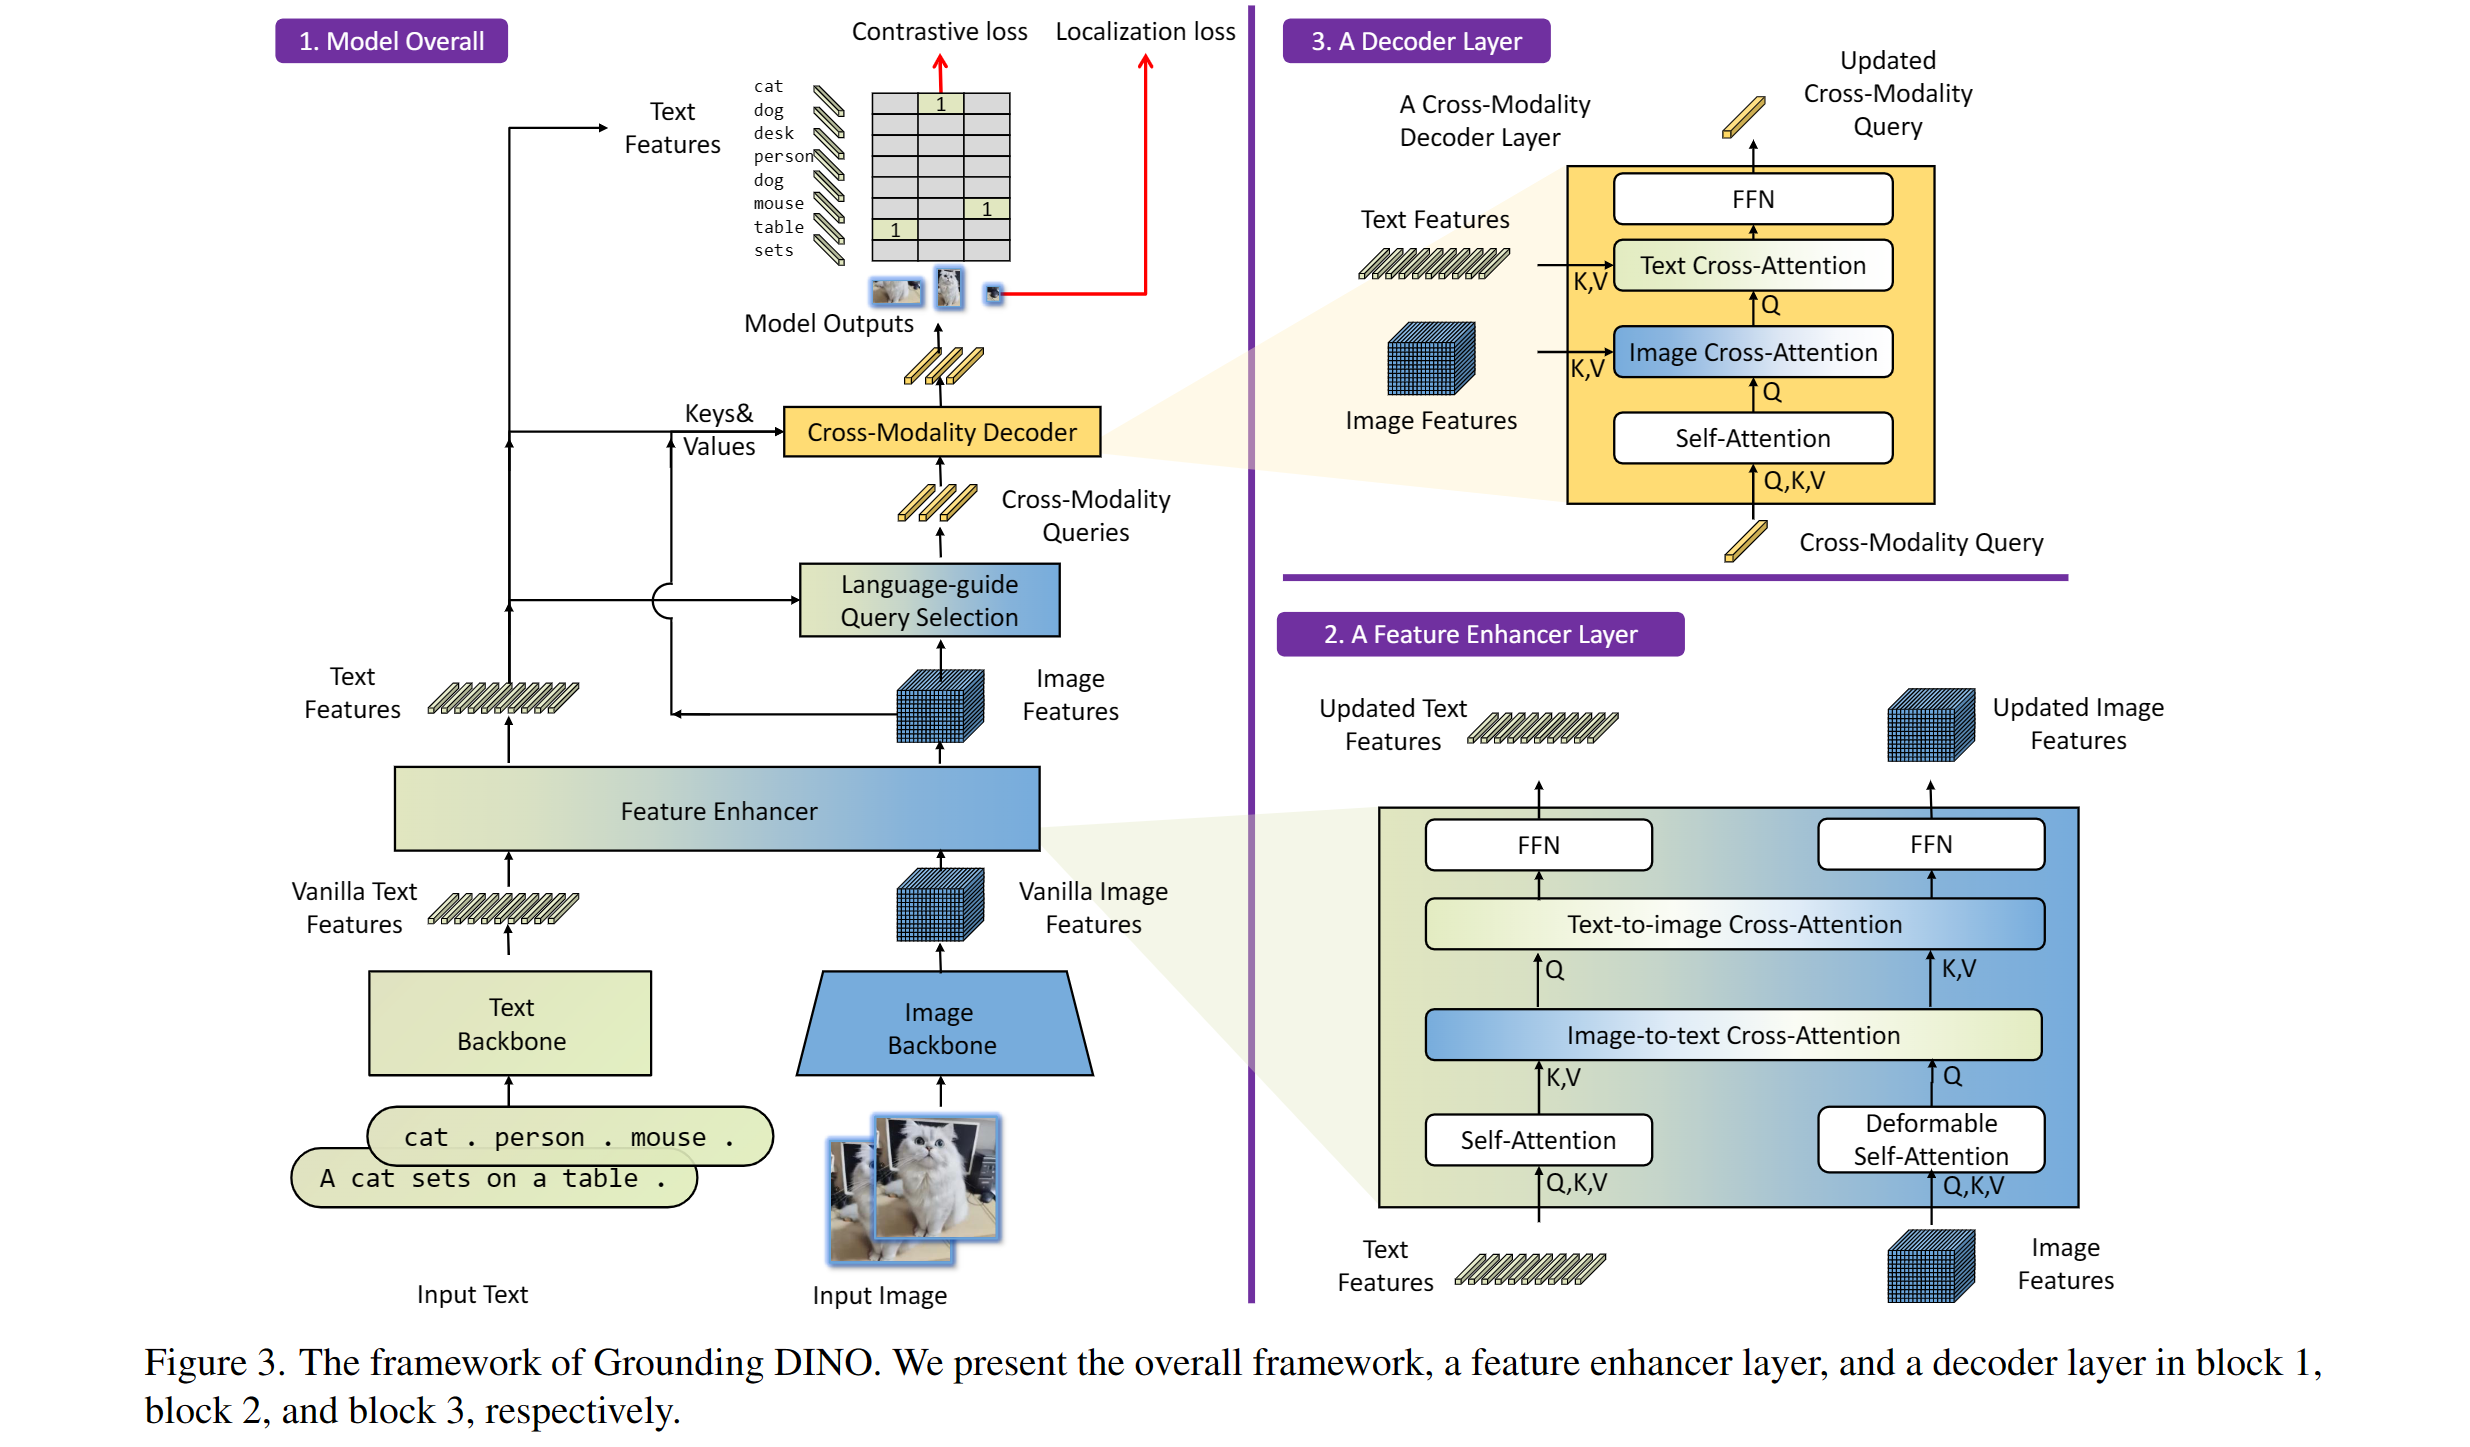
\includegraphics[width=0.8\textwidth]{images/groundingDino.png}
    \caption{Grounding DINO architecture overview with image/text encoders, cross-modal fusion, and language-guided detection outputs.}
    \label{fig:grounding_dino_architecture_overview}
\end{figure}

\paragraph{Language-guided query selection (mathematical intuition).}
Let image tokens be $\mathbf{X}_I\in\mathbb{R}^{N_I\times d}$ and text tokens be $\mathbf{X}_T\in\mathbb{R}^{N_T\times d}$. Grounding DINO selects $N_q$ image indices (typically $N_q=900$) by scoring each image token against the entire text sequence and taking top-$N_q$ locations:
\[
\mathcal{I}_{N_q}=\mathrm{Top}_{N_q}\!\left(\max_{j}(\mathbf{X}_I\mathbf{X}_T^\top)_{:,j}\right).
\]
Intuitively, this implements a soft ``visual saliency under the text prompt'': tokens that strongly align with any word/phrase in the prompt become initialization carriers for object queries \cite{liu2023groundingdino}. The selected indices are then combined with mixed query selection as in DINO: positional components are tied to encoder-derived anchors, while content components remain learnable \cite{liu2023groundingdino}.

\paragraph{Cross-modality decoder.}
Each decoder layer performs self-attention among queries, then updates queries with image cross-attention and an additional text cross-attention pathway. This design repeatedly injects textual constraints during box refinement, rather than conditioning only once \cite{liu2023groundingdino}.

\paragraph{Sub-sentence text representation.}
When prompts concatenate multiple category names, sentence-level encoding can lose token granularity, while naive word-level encoding can introduce spurious dependencies between unrelated words. Grounding DINO introduces a \emph{sub-sentence} representation with attention masks that block interactions between unrelated categories while preserving per-token features \cite{liu2023groundingdino}.


\paragraph{Training objective and matching.}
Grounding DINO follows DETR-style bipartite matching: predicted boxes are matched to ground-truth boxes, and losses are computed on matched pairs. Box regression uses $\ell_1$ and GIoU terms, while classification is treated as a contrastive problem between queries and text tokens with a focal loss on token logits \cite{liu2023groundingdino}. Auxiliary losses after encoder and intermediate decoder layers stabilize deep transformer training \cite{liu2023groundingdino}. The model is pre-trained on heterogeneous detection, grounding, and caption-style data with large-scale grounded supervision, which supports zero-shot transfer on benchmarks such as COCO, LVIS, ODinW, and referring-expression tasks \cite{liu2023groundingdino}. In this thesis, a short text prompt (e.g.\ ``wooden chair'' or ``laptop screen'') is sufficient to obtain candidate boxes on each view without scene-specific fine-tuning.

\subsection{SAM2}
SAM~2 is a foundation model for \emph{promptable visual segmentation} (PVS) that unifies interactive segmentation in images and videos \cite{ravi2024sam2}. A video is treated as a sequence of frames; an image is the special case of a one-frame sequence \cite{ravi2024sam2}.

\paragraph{Task definition: from SAM (image) to masklets (video).}
The PVS task accepts prompts on any frame, points, boxes, or masks, and produces a spatio-temporal mask (\emph{masklet}) for the target entity across frames \cite{ravi2024sam2}. This generalizes interactive video object segmentation: users can correct errors on later frames without restarting from scratch, because the model retains memory of prior prompts and predictions \cite{ravi2024sam2}.


\paragraph{Architecture.}
SAM~2 processes frames in a streaming fashion, consuming one frame at a time \cite{ravi2024sam2}. The main components are the following.

\textbf{Image encoder.} An MAE-pretrained hierarchical Hiera backbone runs once per frame and produces unconditioned, multi-scale spatial feature tokens \cite{ravi2024sam2}. High-resolution skip connections from the encoder bypass memory attention and feed directly into the mask decoder to preserve fine boundary detail.

\textbf{Memory attention.} A stack of $L$ transformer blocks conditions the current-frame tokens on a memory bank. Each block applies self-attention over the current-frame tokens, then cross-attention to stored spatial memories and to lightweight \emph{object pointer} vectors, followed by an MLP \cite{ravi2024sam2}. Vanilla attention is used throughout, enabling compatibility with efficient attention kernels.

\textbf{Prompt encoder and mask decoder.} The prompt encoder is identical to SAM's: sparse inputs (clicks, boxes) are represented as positional encodings summed with learned per-type embeddings, while mask prompts are embedded via convolutions. The decoder uses stacked two-way transformer blocks that jointly update prompt tokens and frame embeddings, and predicts multiple candidate masks under ambiguous prompts; the mask with highest predicted IoU is propagated when no corrective prompt resolves ambiguity \cite{ravi2024sam2}. A dedicated binary head predicts whether the target object is visible on the current frame, handling occlusion transparently.

\textbf{Memory encoder and memory bank.} After decoding, the memory encoder compresses the predicted mask by downsampling it with a convolutional module and adding it element-wise to the unconditioned frame embedding, followed by lightweight convolutional fusion layers \cite{ravi2024sam2}. The resulting spatial feature map is stored in a FIFO queue of up to $N$ recent frames; prompted frames are stored in a separate FIFO queue of up to $M$ slots. Temporal position encodings are added only to the $N$ recent-frame memories (to represent short-term motion), not to prompted-frame memories, because prompted frames may be temporally irregular at inference \cite{ravi2024sam2}.

\begin{figure}[H]
    \centering
    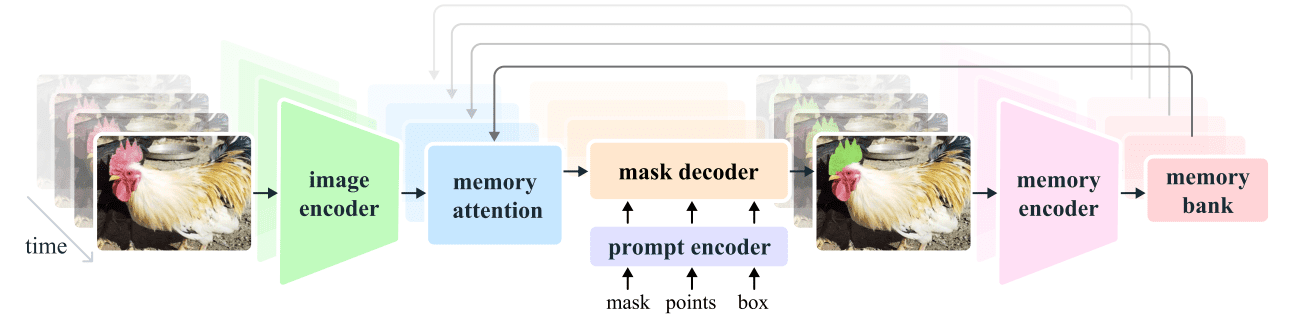
\includegraphics[width=0.95\textwidth]{images/sam2-architecture.png}
    \caption{SAM~2 streaming architecture with memory bank and memory attention for promptable segmentation across frames.}
    \label{fig:sam2_memory_bank_attention}
\end{figure}

\paragraph{Training and data.}
SAM~2 is trained jointly on images and short video clips by simulating interactive prompting: the model receives progressively richer prompts (mask, click, or box with prescribed probabilities) and is trained to sequentially predict ground-truth masklets, including corrective clicks sampled from disagreement regions \cite{ravi2024sam2}. Training is supported by a model-in-the-loop annotation engine that scales collection of diverse masklets, producing the SA-V dataset at a scale substantially larger than prior video segmentation datasets \cite{ravi2024sam2}.

\paragraph{Use in this thesis.}
In the implementation described in Chapter~\ref{chap:methodology}, SAM~2 is invoked through \texttt{SAM2ImagePredictor}: each training image is processed independently, prompted with the bounding box produced by Grounding DINO for that view. The temporal memory bank, which SAM~2 uses for video propagation, is therefore not activated. SAM~2 is used here purely for its strong single-image segmentation quality, which inherits from training on large and diverse data while remaining compatible with the unordered multi-view image collections produced by COLMAP.


\chapter{Tools and Frameworks}
\label{chap:tools}

This chapter describes how the components introduced in Chapter~2 are assembled into a single pipeline: COLMAP-based preprocessing, Nerfstudio training with Splatfacto, optional Hub-hosted depth and segmentation models (Section~\ref{sec:huggingface}), and lightweight geometry utilities. Chapter~\ref{chap:methodology} documents the method-specific extensions applied on top of this stack.

\section{Data preparation}
\label{sec:data_preparation}

The SfM stages were outlined in Chapter~2; here the focus is on the Nerfstudio wrapper around COLMAP. Preprocessing starts with \texttt{ns-process-data images} (or \texttt{video}), implemented by \texttt{Colmap\-Converter\-To\-Nerfstudio\-Dataset} and \texttt{run\_colmap} under \filepath{nerfstudio/process\_data/}. The helper invokes the external \texttt{colmap} binary in sequence: SIFT \texttt{feature\_extractor} (default camera model \texttt{perspective}), a matcher (\texttt{vocab\_tree}, \texttt{exhaustive}, or \texttt{sequential} for ordered video), incremental \texttt{mapper}, and optionally \texttt{bundle\_adjuster} for intrinsic refinement. The resulting folder contains \filepath{colmap/sparse/} (with COLMAP-native \filepath{points3D.bin} or \filepath{points3D.txt}), a converted \filepath{sparse\_pc.ply} used to seed Gaussian means, and \filepath{transforms.json}.

The manifest stores global intrinsics (\texttt{fl\_x}, \texttt{fl\_y}, \texttt{cx}, \texttt{cy}, distortion coefficients, image dimensions). Each frame entry lists a \texttt{file\_path} and a $4\times4$ camera pose stored as \texttt{transform\_matrix}. Dataparsers convert these fields into batched \texttt{Cameras} tensors. Existing COLMAP reconstructions can be ingested without re-running SfM; packaged benchmark scenes are available via \texttt{ns-download-data}.

\section{Nerfstudio and Splatfacto}
\label{sec:splatfacto_gsplat}

Nerfstudio \cite{tancik2023nerfstudio} organizes experiments behind typed \code{@dataclass} configs, swappable \code{DataParser}/\code{DataManager}/\code{Model} components, and a \code{Pipeline} that forwards \code{get\_train\_loss\_dict} to a shared trainer. User commands (\code{ns-process-data}, \code{ns-train}, \code{ns-export}, \code{ns-viewer}, among others) are registered as console scripts in \code{pyproject.toml}.\footnote{\url{https://docs.nerf.studio/}}

\begin{figure}[H]
    \centering
    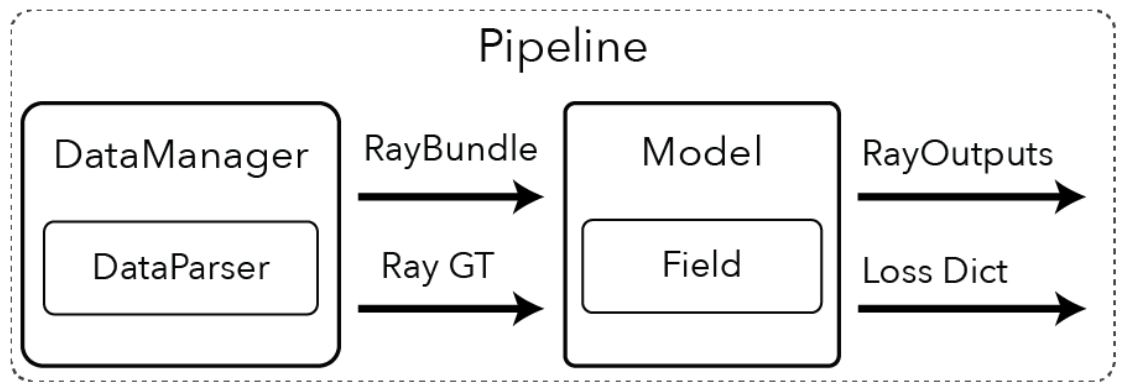
\includegraphics[width=0.85\textwidth]{images/nergstudio.png}
    \caption[Nerfstudio training pipeline]{Nerfstudio training flow: a \code{DataParser} loads disk data, a \code{DataManager} batches viewpoints, and a \code{Model} returns losses. Splatfacto swaps ray bundles for full-frame \code{Cameras} and replaces the MLP \code{Field} with explicit Gaussian parameters.}
    \label{fig:nerfstudio_pipeline}
\end{figure}

The method used throughout this thesis is \textbf{Splatfacto}, the 3D Gaussian Splatting implementation in Nerfstudio \cite{kerbl2023gaussian}. Scene geometry is stored as explicit per-Gaussian tensors (means, covariances, spherical-harmonic colors, opacities) inside \code{SplatfactoModel}; rendering and optimization use \code{FullImageDataManager}, which supplies undistorted full-frame RGB at each step. Differentiable rasterization is delegated to \code{gsplat}, whose CUDA kernels are JIT-compiled on first execution atop PyTorch.

Gaussian means are initialized from the sparse point cloud (\filepath{sparse\_pc.ply}, derived from COLMAP triangulation) when \filepath{transforms.json} is present. Trained checkpoints can be inspected in the Nerfstudio web viewer or exported to \textbf{SuperSplat} \cite{supersplat2024} for interactive inspection of Gaussian centers, ellipsoid geometry, and splat rendering (\url{https://superspl.at/}).

\section{Pretrained models (Hugging Face Hub)}
\label{sec:huggingface}

By default, the pretrained models invoked in this thesis are not vendored as local checkpoints inside the repository. Instead, weights and configuration files are resolved at runtime through the \textbf{Hugging Face Hub}\footnote{\url{https://huggingface.co}}. Each model is identified by a repository id and loaded with \texttt{from\_pretrained(...)}, which downloads or reuses a cached snapshot on first use. Examples include \codeid{depth-anything/da3metric-large} and \codeid{IDEA-Research/grounding-dino-base}.

\subsection{Depth Anything 3 (metric depth)}
Monocular metric depth for supervision and visualization is provided by \texttt{Depth\-Anything3} via \texttt{from\_pretrained} in \filepath{nerfstudio/models/da3\_depth.py}. The default checkpoint is \textbf{DA3METRIC-LARGE} (\codeid{depth-anything/da3metric-large}). During preprocessing (\texttt{ns-process-data} with DA3 depth export) or inside Splatfacto when \texttt{loss=depth}, the wrapper passes each RGB frame and the COLMAP focal length in pixels to obtain a dense depth map in meters.

\subsection{Grounding DINO and SAM~2 (segmentation)}
Object-centric masks rely on two additional Hub-hosted models, implemented in \filepath{nerfstudio/models/sam2\_semantics.py}:
\begin{itemize}
    \item \textbf{Grounding DINO} is loaded via \texttt{transformers} (\texttt{Auto\-Processor} and \texttt{Auto\-Model\-For\-Zero\-Shot\-Object\-Detection.from\_pretrained}), using \codeid{IDEA-Research/grounding-dino-base} by default unless overridden in the Splatfacto config.
    \item \textbf{SAM~2} is loaded through \texttt{SAM2\-Image\-Predictor.from\_pretrained} with a configurable Hub id (for example \codeid{facebook/sam2-hiera-large}), then prompted with boxes from Grounding DINO to obtain per-view binary masks.
\end{itemize}
The same Hub id pins weights across machines; Nerfstudio handles orchestration and loss integration only.

\section{Auxiliary tools}

In this thesis, Open3D \cite{zhou2018open3d} is used to export and inspect the learned B\'ezier surfaces. At the end of training (\texttt{export\_bezier\_meshes}), each patch is sampled on a uniform $(u,v)$ grid; the resulting 3D points are the mesh vertices, and a regular grid triangulation yields triangle faces. Open3D assembles this as a \texttt{TriangleMesh} and writes PLY files (outer, inner, and shell variants when applicable), which can then be opened in any 3D viewer for qualitative inspection. Nerfstudio also uses Open3D elsewhere (e.g.\ loading \filepath{sparse\_pc.ply} for Gaussian initialization), but that path is unrelated to the B\'ezier surface exports described here.


\chapter{Methodology}
\label{chap:methodology}

\section{Baseline: Classical 3D Gaussian Splatting}
\label{sec:baseline_3dgs}

All extensions developed in this thesis are evaluated against a \emph{classical} 3D Gaussian Splatting baseline implemented as Nerfstudio's \textbf{Splatfacto} method (\texttt{splatfacto}), with default configuration \texttt{loss=rgb} and no depth term, semantic masks, or B\'ezier reparameterization. Unless stated otherwise, experiments use the same data preparation pipeline (COLMAP $\rightarrow$ \filepath{transforms.json}) and the same \texttt{FullImageDataManager}. Baseline and depth-supervised runs retain upstream Splatfacto's adaptive clone/split/prune densification \cite{kerbl2023gaussian,tancik2023nerfstudio}; B\'ezier runs disable densification and optimize a fixed $(N_u,N_v)$ lattice on each patch instead (Section~\ref{subsec:bezier_pipeline}).

\subsection{Photometric Loss}
\label{subsec:baseline_photometric}

Baseline training optimizes only image consistency. For each sampled training camera $V$ with ground-truth RGB $I_{\mathrm{gt}}$, Splatfacto rasterizes the current Gaussian set and obtains $\hat{I}$. The objective matches the formulation in Section~2.3.5:
\begin{align}
\mathcal{L}_{\mathrm{rgb}} &= (1-\lambda)\,\mathcal{L}_{1}+\lambda\,\mathcal{L}_{\text{D-SSIM}}, \\
\mathcal{L}_{1} &= \|\hat{I}-I_{\mathrm{gt}}\|_{1}, \\
\mathcal{L}_{\text{D-SSIM}} &= \frac{1-\mathrm{SSIM}(\hat{I},I_{\mathrm{gt}})}{2},
\label{eq:baseline_photometric}
\end{align}
with $\lambda=0.2$ (\code{ssim\_lambda} in the default configuration). Gradients flow back through the differentiable \code{gsplat} rasterizer to update Gaussian means, covariances (via quaternion and log-scale parameters), opacities, and spherical-harmonic color coefficients. Camera poses are optionally refined by the standard Nerfstudio camera optimizer; no auxiliary geometric loss is active in this mode.

This photometric-only setting defines the reference against which depth supervision (Section~\ref{sec:depth_supervised}) and B\'ezier-based structural changes (Section~\ref{sec:bezier_structural}) are motivated; B\'ezier outcomes are evaluated in Chapter~\ref{chap:results}.

\begin{figure}[H]
    \centering
    
\includegraphics[width=0.92\textwidth]{{images/methodology/3d_gaussian viewer_output.png}}
    \caption{Baseline Splatfacto checkpoint exported and inspected in \textbf{SuperSplat} \cite{supersplat2024}, a web-based 3DGS viewer (\url{https://superspl.at/}).
    \textbf{Top left:} scene render with semi-transparent Gaussian splats (unstructured early or diagnostic view).
    \textbf{Top right:} shaded RGB rendering of the reconstructed scene.
    \textbf{Bottom left:} Gaussian \emph{centers} visualized as point sprites (``puntini'') overlaid on the render.
    \textbf{Bottom right:} anisotropic Gaussian \emph{ellipsoids} drawn with wireframe contours, showing the extent and orientation of each primitive.}
    \label{fig:baseline_viewer_outputs}
\end{figure}

\subsection{Expected Depth Estimation}
\label{subsec:baseline_expected_depth}

Although the baseline \emph{loss} does not supervise depth, rendered depth maps are still useful for analysis, export, and as the prediction target when \texttt{loss=depth} is enabled later. Following the volume-rendering viewpoint in Section~2.4.1, each pixel corresponds to a discrete set of front-to-back contributions with compositing weights $w_i=\alpha_i T_i$. The \emph{expected depth} along the viewing direction is
\begin{equation}
d^{\mathrm{exp}}_{x,y}=\frac{\sum_i z_i\,w_i}{\sum_i w_i},
\label{eq:baseline_depth_expected}
\end{equation}
where $z_i$ is the depth coordinate associated with Gaussian $i$ (in the implementation, camera $z$-depth in meters).

In Splatfacto, this quantity is obtained from the \texttt{gsplat} rasterizer by setting \texttt{render\_mode="RGB+ED"}: the fourth channel of the render buffer is the alpha-weighted expected depth, masked where accumulation $\alpha$ is zero. During baseline training (\texttt{loss=rgb}, \texttt{output\_depth\_during\_training=False}), depth is \emph{not} computed on every step to save memory; it is produced at evaluation time and can be exported at the end of training (\texttt{export\_outputs}).

\begin{figure}[H]
    \centering
    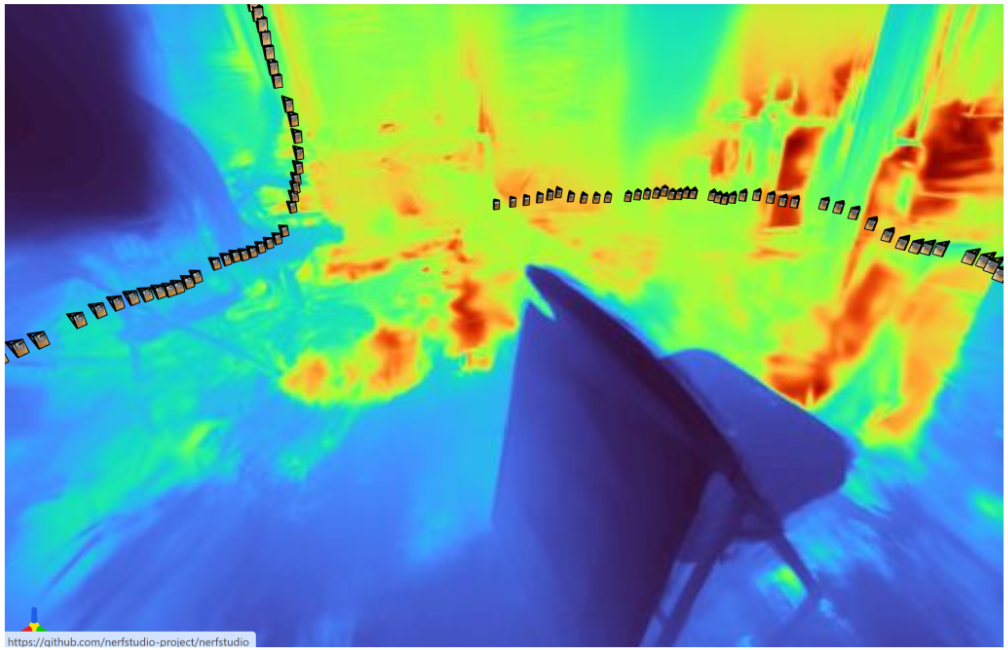
\includegraphics[width=0.85\textwidth]{images/methodology/3dgaussian_expected_depth_out.png}
    \caption{Expected depth $d^{\mathrm{exp}}$ from the baseline rasterizer (\texttt{RGB+ED}), visualized in the Nerfstudio viewer as a false-color map together with the training camera poses. Closer surfaces appear in cooler colors and farther ones in warmer colors (default \texttt{turbo} colormap); background and low-accumulation pixels remain dark. This map is used later as the rendered-depth target when \texttt{loss=depth} is enabled (Section~\ref{sec:depth_supervised}).}
    \label{fig:baseline_expected_depth}
\end{figure}

The codebase also exposes an optional \textbf{ellipsoid depth} mode (\texttt{depth\_mode="ellipsoid"}), which returns the depth of the first ray--ellipsoid hit above a Mahalanobis threshold; it was implemented for diagnostic comparison but is not used in any experiment reported here.

\subsection{Observed Geometric Limitations}
\label{subsec:baseline_limitations}

Empirically, baseline models trained with $\mathcal{L}_{\mathrm{rgb}}$ alone often reach high PSNR/SSIM while yielding unstable explicit geometry. As discussed in Section~2.3.7, 3DGS optimizes photometric consistency rather than explicit surface regularity: several Gaussians can overlap along the same viewing ray, expected depth can look locally sharp while the global depth field stays compressed or inconsistent across views, and exports (point clouds, meshes) remain noisy in low-texture, occluded, or poorly observed regions (Figures~\ref{fig:baseline_viewer_outputs} and~\ref{fig:baseline_expected_depth}).

Detached high-opacity primitives---\emph{floaters} (Figure~\ref{fig:floaters_example})---are one visible symptom of this mismatch, especially behind reflective or transparent surfaces and along depth discontinuities, but they are neither necessary nor sufficient to explain poor geometry on their own. The same photometric objective also encourages broader anisotropic blobs and depth stratification that need not correspond to a single physical surface.

High photometric scores are therefore a weak indicator of metric geometry on their own. The rest of the chapter contrasts two complementary responses against this baseline. Section~\ref{sec:depth_supervised} keeps the classical Gaussian cloud and adds a global depth prior (DA3) on the rendered expected depth $d^{\mathrm{exp}}$, biasing layout toward a dense metric field while leaving densification and free primitive placement unchanged. Section~\ref{sec:bezier_structural} takes a different route: semantically isolated object seeds (Grounding DINO and SAM~2) are fitted with B\'ezier patches and Gaussians are seeded on a fixed $(u,v)$ lattice, trading full-scene flexibility for an explicit, exportable surface on the target object.

\section{Depth-Supervised Optimization}
\label{sec:depth_supervised}

The second methodological extension replaces the photometric $L_1$ term of Section~\ref{sec:baseline_3dgs} with a depth-consistency term, while keeping the same Gaussian parameterization, densification schedule, and COLMAP-based initialization. Training is activated by setting \texttt{loss=depth} in \texttt{SplatfactoModelConfig}; the predicted depth is the rasterizer expected depth $d^{\mathrm{exp}}$ (Eq.~\eqref{eq:baseline_depth_expected}), and the target is a monocular \emph{metric} prior from Depth Anything~3 (DA3METRIC-LARGE, Section~2.4.3).

\subsection{Ground Truth Depth Generation}
\label{subsec:da3_gt_depth}

Unlike relative-depth models (e.g.\ Depth Anything~V2 \cite{yang2024depthanythingv2}), which require per-image scale--shift alignment before supervision, this work uses the \textbf{DA3 metric} checkpoint \codeid{depth-anything/da3metric-large}. For each training RGB image $I$ with known focal length $f$ in pixels (from COLMAP intrinsics), DA3 returns a network output $\hat{d}_{\mathrm{net}}$ that is converted to metric camera depth in meters by
\begin{equation}
d_{\mathrm{DA3}} = \frac{f\,\hat{d}_{\mathrm{net}}}{300},
\label{eq:da3_metric}
\end{equation}
following the model-card convention implemented in \filepath{nerfstudio/models/da3\_depth.py}. Depth is inferred \emph{independently per view}; multi-view cross-attention and ray-map outputs of the full DA3 framework are not used at training time (Section~2.4.3).

\paragraph{Preprocessing and caching.}
Ground-truth depth maps can be materialized offline during dataset conversion (\code{ns-process-data images --use-da3-depth}), which writes 16-bit PNGs under \filepath{depth/} and registers them in \filepath{transforms.json}. At training time, Splatfacto first reads \code{batch["depth\_image"]} when present; otherwise it falls back to on-the-fly DA3 inference with an in-memory (and optional on-disk) cache keyed by camera index.

\begin{lstlisting}[caption={Metric conversion in \code{DA3MetricDepthEstimator.infer\_metric\_depth} (\filepath{da3\_depth.py}).},label={lst:da3_metric}]
pred = model.inference([img_uint8]).depth[0]   # network output
metric = (pred * focal_px) / 300.0             # meters, per DA3METRIC-LARGE
\end{lstlisting}

\begin{figure}[H]
    \centering
    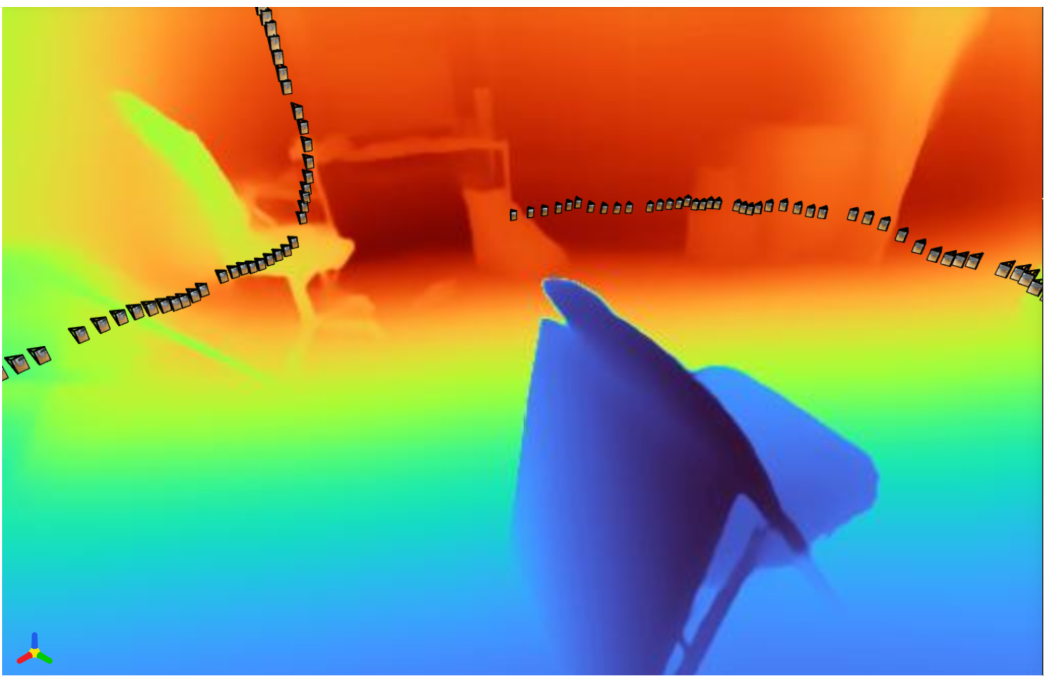
\includegraphics[width=0.75\textwidth]{images/methodology/dav3_output.png}
    \caption{Example DA3 metric depth target ($d_{\mathrm{DA3}}$) visualized in the Nerfstudio viewer for one training view. Warmer colors denote larger camera $z$-depth.}
    \label{fig:da3_depth_target}
\end{figure}

\subsection{Depth Loss Formulation}
\label{subsec:depth_loss}

When \texttt{loss=depth}, the main training objective supervises rendered depth instead of RGB. Let $d^{\mathrm{exp}}$ be the expected depth from \texttt{render\_mode="RGB+ED"} and $d_{\mathrm{DA3}}$ the pseudo ground truth for the same view (resampled to the current training resolution). The primary loss is
\begin{equation}
\mathcal{L}_{\mathrm{depth}} = \frac{1}{|\Omega|}\sum_{(x,y)\in\Omega}\left|d^{\mathrm{exp}}_{x,y}-d_{\mathrm{DA3},x,y}\right|,
\label{eq:depth_loss}
\end{equation}
where $\Omega$ is the set of valid pixels (optionally restricted by a segmentation mask). Importantly, the D-SSIM term on RGB is \textbf{not} added in this mode: appearance is no longer directly optimized at each step, although RGB is still rendered for logging and evaluation.

\begin{lstlisting}[caption={Depth branch in \texttt{SplatfactoModel.get\_loss\_dict} (\filepath{splatfacto.py}).},label={lst:depth_loss_code}]
if self.config.loss == "depth":
    pred_depth = outputs["depth"]          # RGB+ED expected depth
    gt_depth = batch["depth_image"]        # or DA3 on-the-fly
    Ll1 = torch.abs(gt_depth - pred_depth).mean()
    loss_dict = {"main_loss": Ll1, ...}   # no SSIM term
else:
    Ll1 = torch.abs(gt_img - pred_img).mean()
    simloss = 1 - self.ssim(gt_img, pred_img)
    loss_dict = {"main_loss": (1-lambda)*Ll1 + lambda*simloss, ...}
\end{lstlisting}

Gradients therefore flow primarily into Gaussian positions, scales, and opacities (the parameters that influence $d^{\mathrm{exp}}$), rather than into spherical-harmonic color coefficients.

\subsection{Joint Optimization Strategy}
\label{subsec:depth_joint_opt}

Apart from the swapped $L_1$ term, the optimization loop is unchanged: adaptive clone/split/prune, optional camera-pose refinement, and the same learning-rate schedules as the RGB baseline. Expected depth is enabled during training (\texttt{output\_depth\_during\_training} implicitly via \texttt{loss=depth}) so that $\mathcal{L}_{\mathrm{depth}}$ can be evaluated every iteration.

\paragraph{Role of COLMAP color initialization.}
A key observation, relevant when comparing RGB and depth renders, is that Gaussian \emph{colors} are initialized from COLMAP tie points, which carry per-point RGB estimates in addition to 3D position. In \texttt{SplatfactoModel.populate\_modules}, the DC spherical-harmonic coefficients are set from these colors via \texttt{RGB2SH} before the first training step. As a result, the scene is already chromatically recognizable at iteration zero, even though $\mathcal{L}_{\mathrm{depth}}$ does not update appearance. This explains why novel-view RGB can look broadly similar between \texttt{loss=rgb} and \texttt{loss=depth} experiments, despite very different geometric gradients.

\begin{lstlisting}[caption={Color initialization from COLMAP seed points (\filepath{splatfacto.py}).},label={lst:colmap_color_init}]
shs[:, 0, :3] = RGB2SH(seed_rgb / 255)   # seed_rgb from sparse SfM points
features_dc = torch.nn.Parameter(shs[:, 0, :])
\end{lstlisting}

\subsection{Qualitative Trade-offs: RGB vs.\ Depth Loss}
\label{subsec:depth_rgb_tradeoff}

Although final RGB images can appear similar because of shared initialization, the \emph{depth maps} and \emph{internal Gaussian layouts} differ markedly between the two loss modes. Figures~\ref{fig:rgb_depth_render_compare} and~\ref{fig:rgb_depth_depth_compare} summarize the behavior observed on the same indoor scene (chair and poster).

\paragraph{Training with $\mathcal{L}_{\mathrm{rgb}}$ (photometric loss).}
The photometric objective forces the model to explain local intensity patterns, object contours, and high-frequency texture. To reduce $\mathcal{L}_{\mathrm{rgb}}$, Gaussians often stratify along the viewing direction in front of salient structures: multiple semi-transparent layers stack in depth and collectively contribute to both color and $d^{\mathrm{exp}}$. On the foreground object, this can yield depth estimates that look locally sharp; however, the background exhibits higher speckle noise, a compressed global depth range, and reduced multi-view coherence. Figure~\ref{fig:supersplat_rgb_vs_depth} (left) shows this effect in SuperSplat: dense overlapping ellipsoids with visible contours along viewing rays.

\paragraph{Training with $\mathcal{L}_{\mathrm{depth}}$ (depth loss).}
Here the optimizer is driven mainly by a \emph{global} depth field. Gaussians tend to collapse their extent along the ray direction and concentrate around a representative depth, producing smoother background depth closer to the DA3 prior range, but at the cost of local geometric ambiguity on the object (blurred structure, missing thin parts, and depth bleeding at discontinuities). In other words, depth supervision improves global depth coherence while being less constrained on fine local geometry; the opposite trade-off of photometric training.

\begin{figure}[H]
    \centering
    \begin{subfigure}[b]{0.48\textwidth}
        \centering
        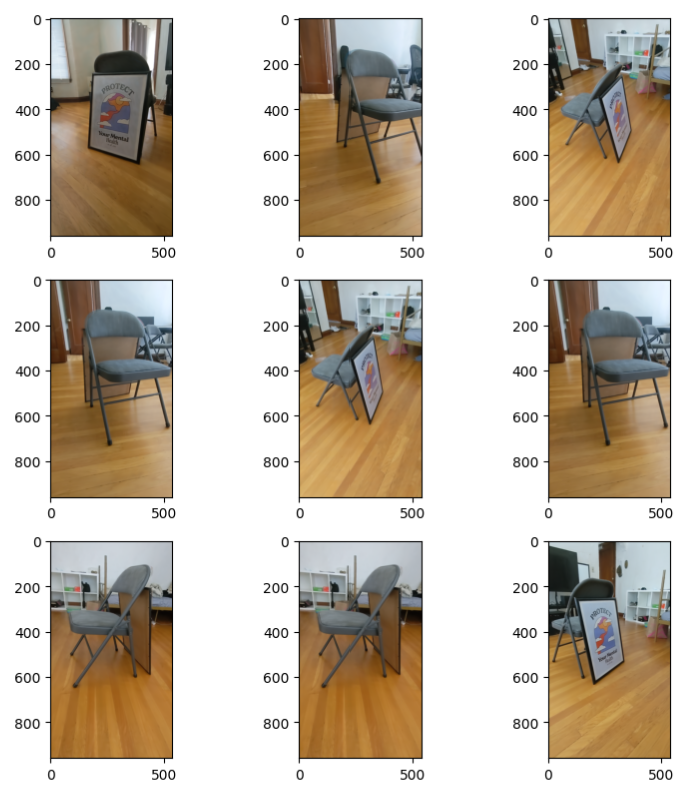
\includegraphics[width=\textwidth]{images/methodology/loss_classica_render_rgb.png}
        \caption{\texttt{loss=rgb}}
        \label{fig:rgb_loss_render}
    \end{subfigure}
    \hfill
    \begin{subfigure}[b]{0.48\textwidth}
        \centering
        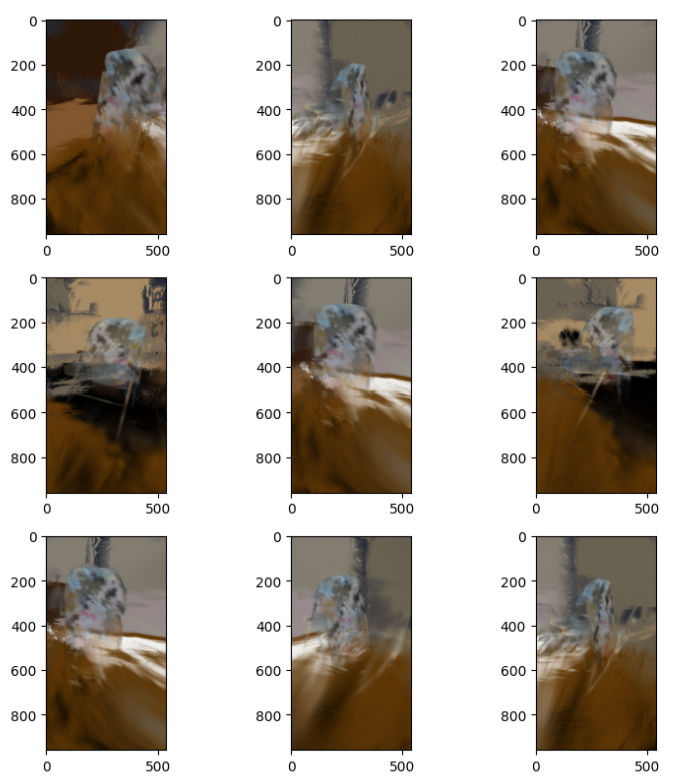
\includegraphics[width=\textwidth]{images/methodology/loss_depth_render_rgb.png}
        \caption{\texttt{loss=depth}}
        \label{fig:depth_loss_render}
    \end{subfigure}
    \caption{Rendered RGB on held-out views after training with photometric loss (left) versus depth loss (right). Overall color layout is similar because both runs share COLMAP color initialization, even though only the left model optimizes appearance.}
    \label{fig:rgb_depth_render_compare}
\end{figure}

\begin{figure}[H]
    \centering
    \begin{subfigure}[b]{0.48\textwidth}
        \centering
        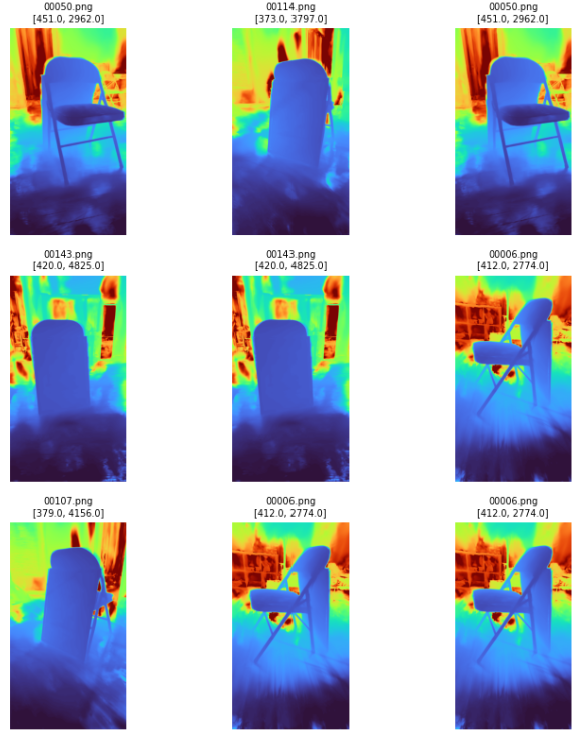
\includegraphics[width=\textwidth]{images/methodology/loss_classica_expected_depth.png}
        \caption{\texttt{loss=rgb}}
        \label{fig:rgb_loss_depthmap}
    \end{subfigure}
    \hfill
    \begin{subfigure}[b]{0.48\textwidth}
        \centering
        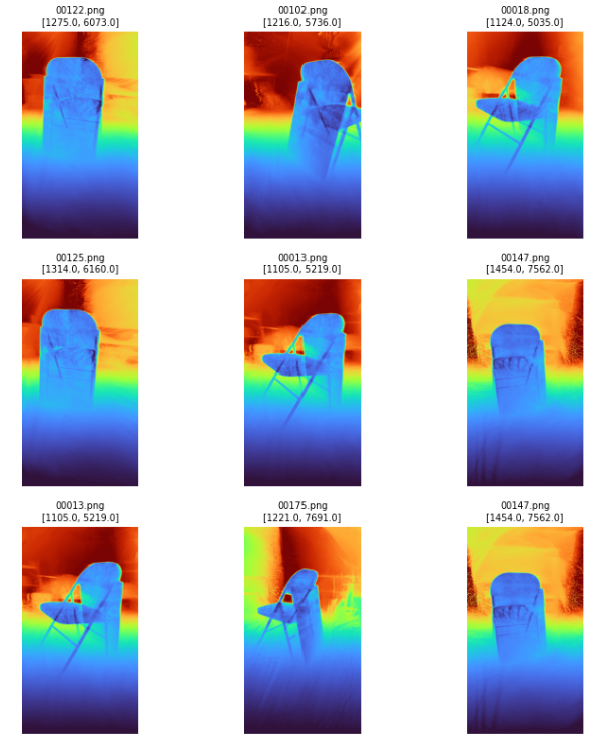
\includegraphics[width=\textwidth]{images/methodology/loss_depth_expected_depth.png}
        \caption{\texttt{loss=depth}}
        \label{fig:depth_loss_depthmap}
    \end{subfigure}
    \caption{Exported expected depth $d^{\mathrm{exp}}$ for the same scene: photometric training (left) shows sharper object silhouettes but noisier background and a narrower effective depth range; depth training (right) yields smoother background depth closer to the DA3 prior, with softer object detail.}
    \label{fig:rgb_depth_depth_compare}
\end{figure}

\begin{figure}[H]
    \centering
    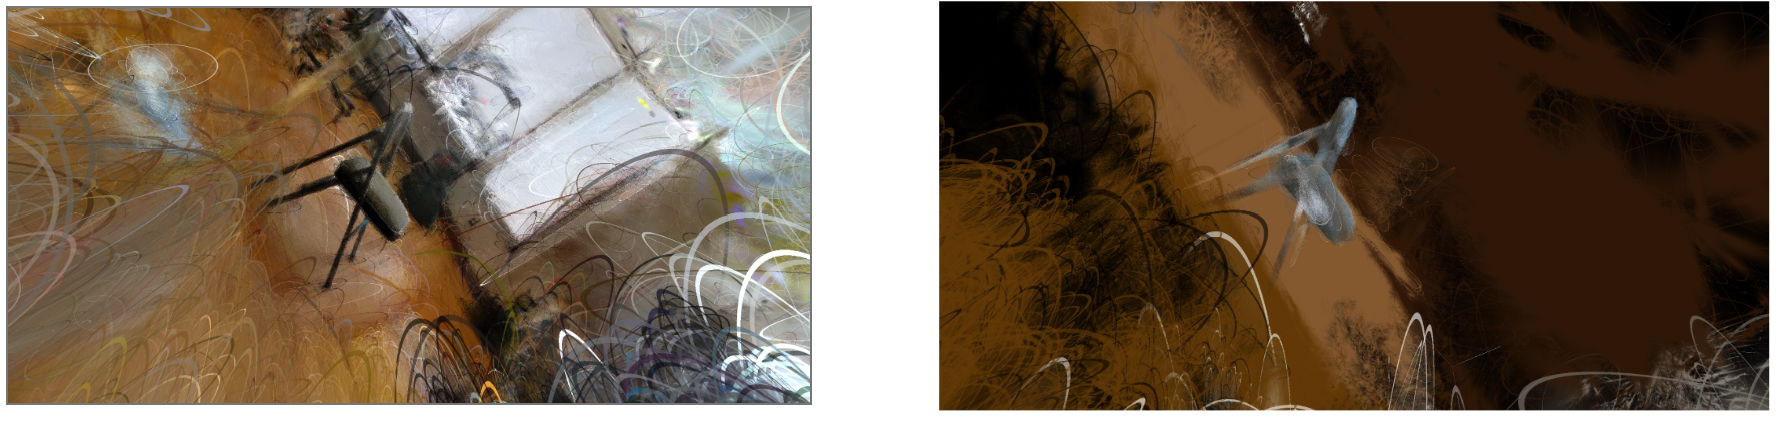
\includegraphics[width=0.92\textwidth]{images/methodology/render_class+render_depth_viewer.png}
    \caption[SuperSplat: RGB vs.\ depth loss]{\textbf{SuperSplat} \cite{supersplat2024} comparison with ellipsoid wireframes.
    \textbf{Left (\code{loss=rgb}):} dense stacks of semi-transparent ellipsoids aligned with viewing rays (stratification in depth).
    \textbf{Right (\code{loss=depth}):} sparser ellipsoid distribution with weaker local layering and reduced structural detail on the foreground object, consistent with a globally smoother depth field.}
    \label{fig:supersplat_rgb_vs_depth}
\end{figure}

\subsection{Failure Modes and Instabilities}
\label{subsec:depth_failure}

Depth supervision inherits limitations of monocular priors: reflective or transparent surfaces, thin structures, and textureless walls can be misestimated by DA3 and then propagated into the Gaussian cloud. Because DA3 depths are computed per view without explicit multi-view fusion, inconsistent pseudo-labels across cameras can create rippling artifacts in $d^{\mathrm{exp}}$. Overly strong depth fitting may also flatten legitimate depth discontinuities (object boundaries), while under-fitting leaves floaters that no longer penalize RGB error.

Practically, $\mathcal{L}_{\mathrm{depth}}$ should be interpreted as a \emph{global geometry regularizer} rather than a replacement for photometric detail. Combining both signals (e.g.\ weighted RGB+$L_1$ depth, or object-masked losses in Section~\ref{sec:bezier_structural}) is left as future work; the present thesis evaluates the two extremes, pure RGB and pure depth, to expose their complementary biases.

\section{Structural Modification via B\'ezier Surfaces}
\label{sec:bezier_structural}

The third methodological axis replaces free 3D Gaussian placement on the full COLMAP cloud with \textbf{object-centric B\'ezier surface patches} \cite{liu2025bezier}. Each patch is a tensor-product B\'ezier surface fitted to a subset of sparse object seed points from the COLMAP point cloud; Gaussians are then sampled on a regular $(u,v)$ grid and optimized jointly with the patch control points. This section covers (i)~how object points are isolated semantically, (ii)~how sparse outliers are removed before fitting, and (iii)~how patches are initialized and coupled to splatting (following subsections).

The pipeline is enabled by \code{bezier\_init\_enabled=True} together with \code{sam2\_semantic\_init\_enabled=True} and a text prompt (e.g.\ \code{sam2\_text\_prompts=["chair"]}). At training startup, \code{VanillaPipeline} runs Grounding DINO + SAM~2, labels COLMAP seed points, and passes \code{metadata["seed\_semantic\_labels"]} to \code{SplatfactoModel} (Section~\ref{sec:huggingface}, Chapter~\ref{chap:tools}).

\subsection{Semantic Object Isolation}
\label{subsec:semantic_isolation}

Object-centric geometry requires associating each COLMAP 3D point $\mathbf{p}_i\in\mathcal{P}$ with a discrete label $\ell_i\in\{0,1,\ldots\}$, where $\ell_i=0$ denotes background and $\ell_i>0$ an object instance or prompt-specific class. This thesis uses the \textbf{Grounded SAM~2} path implemented in \filepath{nerfstudio/models/sam2\_semantics.py}:

\begin{enumerate}
    \item For each training image $I$, \textbf{Grounding DINO} predicts bounding boxes from a text prompt (Section~2.5.1).
    \item \textbf{SAM~2} (\code{SAM2ImagePredictor}) segments each box into a binary mask; masks from multiple prompts are merged into a per-pixel \emph{label map} with prompt-priority rules (later prompts do not overwrite pixels already labeled).
    \item COLMAP 2D tracks (\code{points3D\_image\_ids}, \code{points3D\_points2D\_xy}) project each 3D point into the images where it was observed; the label at the projected pixel votes for that point.
    \item Votes accumulated across all segmented views yield a final label per 3D point (majority / first-hit aggregation in \code{\_labels\_from\_labelmap\_votes}).
\end{enumerate}

Only points with $\ell_i>0$ are retained for B\'ezier fitting; background seeds are discarded before patch generation. Masks can also be exported to the dataparser (\code{convert\_sam2\_labelmaps\_to\_binary\_masks}) for optional foreground--background losses during training (Section~\ref{subsec:mask_losses}).

\begin{figure}[H]
    \centering
    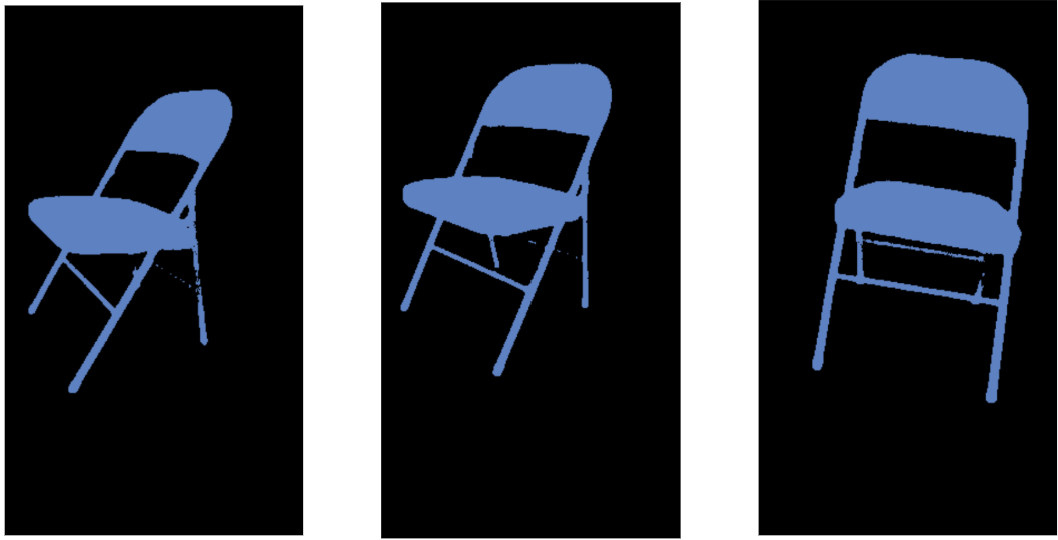
\includegraphics[width=0.92\textwidth]{images/methodology/exaple_segmetation.png}
    \caption{Example SAM~2 masks obtained from a text prompt (here, a chair) on three training views. Each mask defines the image regions that vote for object labels on projected COLMAP seed points.}
    \label{fig:bezier_segmentation_example}
\end{figure}

\paragraph{Configuration.}
Key flags include:
\begin{itemize}
    \item \code{sam2\_text\_prompts};
    \item \code{sam2\_segment\_all\_train\_images} (or an explicit \code{sam2\_segment\_image\_indices} list);
    \item \code{sam2\_segmentation\_output\_dir} (default \filepath{data/grounded\_sam2/}) for label maps and debug visualizations.
\end{itemize}
The dataparser must export full 2D tracks (\code{max\_2D\_matches\_per\_3D\_point} $>0$ or $-1$ for unlimited).

\subsection{Seed Point Preprocessing}
\label{subsec:seed_preprocessing}

Even after semantic filtering, COLMAP triangulation can leave \emph{isolated} seed points far from the object surface; for example, due to matching errors, reflective surfaces, or points on background geometry that received a spurious object label in a single view. Fitting B\'ezier patches to such outliers distorts control nets and produces Gaussians detached from the true shape (Figure~\ref{fig:bezier_outlier_seed}; Figure~\ref{fig:bezier_outliers_output}).

\subsubsection{k-NN Outlier Filtering}
\label{subsec:knn_outlier}

Before patch generation, \texttt{filter\_seed\_points\_outlier\_knn\_mean} in \filepath{splatfacto.py} removes sparse points \emph{per semantic class}. For each label $c$, let $\mathcal{P}_c=\{\mathbf{p}_i:\ell_i=c\}$. For every point $\mathbf{p}_i\in\mathcal{P}_c$, compute the mean distance to its $k$ nearest neighbors within the same class:
\begin{equation}
d_i = \frac{1}{k}\sum_{j=1}^{k}\|\mathbf{p}_i-\mathbf{p}_{i,j}^{(k)}\|,
\qquad
\bar{d}_c = \frac{1}{|\mathcal{P}_c|}\sum_{\mathbf{p}_i\in\mathcal{P}_c} d_i.
\label{eq:knn_mean_dist}
\end{equation}
Point $\mathbf{p}_i$ is kept if $d_i \le \lambda\,\bar{d}_c$ and discarded otherwise, where $\lambda$ and $k$ are set by \code{bezier\_seed\_outlier\_knn\_lambda} and \code{bezier\_seed\_outlier\_knn\_k} (default $k=8$). Setting $\lambda\le 0$ disables filtering. Typical values $\lambda\in[2,3]$ remove only points whose local spacing is far larger than the class average (isolated ``floaters'' in seed space). If all points of a class would be removed, the implementation keeps the full class and logs a warning.

\begin{algorithm}[htbp]
\caption{k-NN outlier filtering of B\'ezier seed points (\code{filter\_seed\_points\_outlier\_knn\_mean})}
\label{alg:knn_outlier}
\begin{algorithmic}[1]
\Require Seed positions $\{\mathbf{p}_i\}$, labels $\{\ell_i\}$, neighbors $k$, multiplier $\lambda$
\Ensure Filtered seeds $(\mathbf{p},\ell)$ with outliers removed per class
\If{$\lambda \le 0$}
    \State \Return all seeds unchanged
\EndIf
\For{each semantic label $c$}
    \State $\mathcal{P}_c \gets \{\mathbf{p}_i : \ell_i = c\}$
    \If{$|\mathcal{P}_c| \le k$}
        \State keep all points in $\mathcal{P}_c$ \Comment{too few points for stable $k$-NN}
    \Else
        \For{each $\mathbf{p}_i \in \mathcal{P}_c$}
            \State $d_i \gets$ mean $\ell_2$ distance to $k$ nearest neighbors in $\mathcal{P}_c$
        \EndFor
        \State $\bar{d}_c \gets \mathrm{mean}_i(d_i)$
        \State keep $\mathbf{p}_i$ iff $d_i \le \lambda\,\bar{d}_c$
    \EndIf
\EndFor
\State \Return concatenation of kept points over all classes
\end{algorithmic}
\end{algorithm}

\begin{lstlisting}[caption={Core loop in \texttt{filter\_seed\_points\_outlier\_knn\_mean} (abridged).},label={lst:knn_outlier}]
dists, _ = k_nearest_sklearn(pts, k)       # (N_c, k) per class
dk = dists.mean(dim=-1)                    # d_i in Eq.~\eqref{eq:knn_mean_dist}
thresh = lambda_mult * dk.mean().clamp_min(1e-8)
keep = dk <= thresh
\end{lstlisting}

The filter is invoked inside \code{SplatfactoModel.populate\_modules} immediately after restricting to object labels ($\ell>0$) and before \code{generate\_bezier\_patches\_from\_labeled\_points} or cube initialization:
\begin{lstlisting}[caption={Call site before B\'ezier patch fitting (\filepath{splatfacto.py}).},label={lst:knn_call}]
seed_xyz_obj, seed_labels_obj, seed_rgb_obj = filter_seed_points_outlier_knn_mean(
    seed_xyz_obj, seed_labels_obj, seed_rgb_obj,
    k=int(self.config.bezier_seed_outlier_knn_k),
    lambda_mult=float(self.config.bezier_seed_outlier_knn_lambda),
)
\end{lstlisting}

\begin{figure}[H]
    \centering
    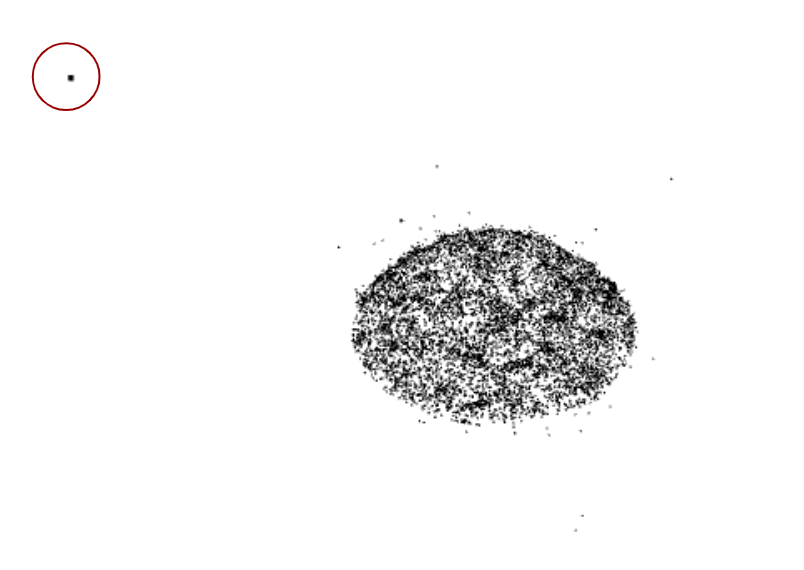
\includegraphics[width=0.55\textwidth]{images/methodology/esempio_outliers.png}
    \caption{Seed outlier \emph{before} $k$-NN filtering: a single mislabeled COLMAP seed (red circle) far from the chair cluster.}
    \label{fig:bezier_outlier_seed}
\end{figure}

\begin{figure}[H]
    \centering
    \begin{subfigure}[b]{0.48\textwidth}
        \centering
        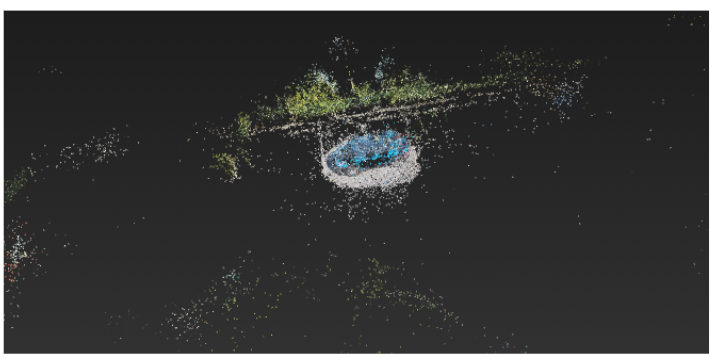
\includegraphics[width=\textwidth]{images/methodology/cloud_point_out.png}
        \caption{Full seed point cloud}
        \label{fig:bezier_outlier_cloud}
    \end{subfigure}
    \hfill
    \begin{subfigure}[b]{0.48\textwidth}
        \centering
        
\includegraphics[width=\textwidth]{{images/methodology/esempio_inizializzazione con outliers.png}}
        \caption{Fitted B\'ezier patches}
        \label{fig:bezier_outlier_gaussians}
    \end{subfigure}
    \caption{B\'ezier initialization when outlier seeds are not removed. \textbf{(a)} COLMAP seed point cloud with all points assigned to the object class (including outliers). \textbf{(b)} 3D visualization of the fitted B\'ezier surfaces warped by those outliers (Open3D).}
    \label{fig:bezier_outliers_output}
\end{figure}

\subsection{B\'ezier Surface Initialization}
\label{subsec:bezier_init}

After semantic filtering and $k$-NN outlier rejection, each object class is represented by one or more tensor-product B\'ezier patches of degree $3\times 3$ (a $4\times 4$ control grid, 16 control points per patch), consistent with Section~2.5.2. This thesis evaluates two \emph{initialization geometries} only:
\begin{itemize}
    \item \textbf{Open-surface mode} (\code{bezier\_init\_enabled=True}, \code{bezier\_cube\_init=False}): patches fitted locally to seed neighborhoods (default \code{bezier\_surface\_mode="open"}).
    \item \textbf{Cube mode} (\code{bezier\_cube\_init=True}): six faces of an axis-aligned bounding box (AABB), each tiled with $k\times k$ patches that share control points on face boundaries and cube edges.
\end{itemize}

\subsubsection{Control Point Estimation}
\label{subsec:bezier_cp_estimation}

\paragraph{Open-surface patches.}
For each semantic label $c$, let $\mathcal{P}_c$ be the filtered seed set. The generator \texttt{generate\_bezier\_patches\_from\_labeled\_points} (\filepath{bezier\_surface.py}) builds \texttt{bezier\_num\_patches\_per\_class} patches as follows:
\begin{enumerate}
    \item \textbf{Patch centers:} select $P$ anchor points in $\mathcal{P}_c$ using farthest-point sampling (FPS, default \texttt{bezier\_center\_sampling="fps"}) or uniform random indices.
    \item \textbf{Local neighborhood:} for each center $\mathbf{c}$, retrieve $K=\texttt{bezier\_knn\_k}$ nearest neighbors in $\mathcal{P}_c$ (typically $K=64$).
    \item \textbf{Planar control grid:} fit a $4\times 4$ control net on the best-fit plane of the neighborhood via PCA (function \texttt{\_create\_planar\_control\_points}): compute the mean $\boldsymbol{\mu}$, take the two principal axes of largest variance, and place control points on a regular grid spanning the projected extent of neighbors in that $(u,v)$ plane. The result is a \emph{planar} initial surface, not a least-squares fit to scattered 3D points.
\end{enumerate}

\begin{algorithm}[htbp]
\caption{Open-mode B\'ezier control-point initialization (per class, per patch)}
\label{alg:bezier_cp_open}
\begin{algorithmic}[1]
\Require Filtered seeds $\mathcal{P}_c$, number of patches $P$, neighbors $K$, grid size $G{=}4$
\State $\mathcal{C} \gets \mathrm{FPS}(\mathcal{P}_c, P)$ \Comment{or random centers}
\For{each center $\mathbf{c} \in \mathcal{C}$}
    \State $\mathcal{N} \gets k\mathrm{NN}(\mathcal{P}_c, \mathbf{c}, K)$
    \State $(\mathbf{u},\mathbf{v}) \gets$ first two principal axes of $\mathcal{N}$ (PCA)
    \State Project $\mathcal{N}$ onto $(\mathbf{u},\mathbf{v})$; build $G\times G$ grid in that plane
    \State Store control net $\mathbf{p}_{i,j}\in\mathbb{R}^3$, $i,j\in\{0,\ldots,G{-}1\}$
\EndFor
\end{algorithmic}
\end{algorithm}

\begin{lstlisting}[caption={Planar control grid from a $k$-NN neighborhood (\filepath{bezier\_surface.py}).},label={lst:planar_cp}]
mu = neighbors.mean(dim=0)
X = neighbors - mu
C = (X.T @ X) / (K - 1)
evecs = torch.linalg.eigh(C).eigenvectors
u_axis, v_axis = evecs[:, -1], evecs[:, -2]
# GxG grid along projected min/max extents -> (G, G, 3) control points
\end{lstlisting}

\paragraph{Cube-mode patches.}
When \code{bezier\_cube\_init=True}, control points are \emph{not} fitted from local neighborhoods. Instead, \code{generate\_bezier\_cube\_from\_labeled\_points} computes the AABB $[\mathbf{b}_{\min},\mathbf{b}_{\max}]$ of $\mathcal{P}_c$, inflates degenerate axes by a tiny margin, and calls \code{build\_cube\_bezier\_control\_points}:
\begin{itemize}
    \item Each of the six box faces carries a regular $n_{\mathrm{cp}}\times n_{\mathrm{cp}}$ lattice of world-space control points, with $n_{\mathrm{cp}} = 3k+1$ for cubic patches ($k=\texttt{bezier\_cube\_k}$ patches per face edge).
    \item Face lattices are concatenated; coincident points at edges and corners are merged via \code{torch.unique}, yielding a single tensor \code{bezier\_cube\_shared\_cp} of unique positions.
    \item An \code{index\_map} of shape $(6k^2,4,4)$ maps each face patch to indices into the shared tensor. Adjacent patches therefore share boundary control points by construction ($C^0$ continuity along cube edges), without a separate ``shell'' or closed-volume model (see Figure~\ref{fig:bezier_cube_box}).
\end{itemize}

\subsubsection{Surface Sampling and Gaussian Seeding}
\label{subsec:bezier_surface_sampling}

Control points define a patch $\mathbf{S}(u,v)$ via Bernstein blending (Section~2.5.2, Figure~\ref{fig:bezier_surface_example}). At initialization, each patch is uniformly sampled on
\begin{align}
u_i &= \frac{i}{N_u-1},\quad v_j = \frac{j}{N_v-1}, \\
i &\in \{0,\ldots,N_u-1\},\quad j \in \{0,\ldots,N_v-1\},
\end{align}
with $N_u=\texttt{bezier\_num\_u}$ and $N_v=\texttt{bezier\_num\_v}$ (defaults $20\times 20$). Sample positions $\mathbf{x}_{i,j}=\mathbf{S}(u_i,v_j)$ become Gaussian \textbf{means}.

\paragraph{Local tangent frame.}
For each sample, central finite differences on the grid approximate partial tangents $\partial_u\mathbf{S}$ and $\partial_v\mathbf{S}$; border samples use forward/backward stencils. Unit tangents $\mathbf{t}_u,\mathbf{t}_v$ and normal $\mathbf{n}=\mathbf{t}_u\times\mathbf{t}_v$ (re-orthogonalized) form a rotation matrix $\mathbf{R}=[\mathbf{t}_u\;\mathbf{t}_v\;\mathbf{n}]$, converted to quaternions for \texttt{gsplat}. This aligns each Gaussian's anisotropy with the local surface geometry.

\paragraph{Anisotropic scales.}
In the local frame $\mathbf{R}=[\mathbf{t}_u\;\mathbf{t}_v\;\mathbf{n}]$, each ellipsoid has semi-axis lengths $(\sigma_u,\sigma_v,\sigma_n)$ along the tangent directions and the surface normal. Adjacent sample spacing on the patch sets the \emph{tangential} extents; $\rho$ and $\alpha$ map grid spacing to world-space axis lengths:
\[
\sigma_u = \frac{\|\mathbf{x}_{i+1,j}-\mathbf{x}_{i,j}\|}{\rho},\qquad
\sigma_v = \frac{\|\mathbf{x}_{i,j+1}-\mathbf{x}_{i,j}\|}{\rho},
\qquad
\sigma_n = \frac{\alpha}{\rho},
\]
with $\rho=\texttt{bezier\_rho}$ (default $20$) and $\alpha=\texttt{bezier\_alpha}$ (default $1$). Thus $\rho$ shrinks or enlarges the in-plane footprint relative to the distance between lattice samples (larger $\rho$ $\Rightarrow$ narrower splats along $\mathbf{t}_u,\mathbf{t}_v$ and more overlap between neighbors on the surface), whereas $\alpha$ sets the initial \emph{normal} thickness $\sigma_n$ independently of local spacing (larger $\alpha$ $\Rightarrow$ thicker support off the surface). Log-scales passed to \texttt{gsplat} are $\log(\sigma_u,\sigma_v,\sigma_n)$.

\paragraph{Appearance and semantics.}
Per-patch color is the mean RGB of seed points in that semantic class; all $N_u N_v$ Gaussians on the patch inherit it as flat SH DC coefficients (\texttt{RGB2SH}), with higher bands zero unless \texttt{patch\_textures} override color each forward (Section~\ref{subsec:bezier_textures}). Semantic labels are stored in \code{gaussian\_semantic\_labels}. In \textbf{open mode}, the $4\times 4$ control nets are registered as \code{bezier\_open\_cp} and re-sampled every forward pass so rendering gradients update geometry. In \textbf{cube mode}, \code{bezier\_cube\_shared\_cp} plays the same role with patches indexed through \code{bezier\_cube\_index\_map}.

\begin{algorithm}[htbp]
\caption{From B\'ezier patch samples to initial Gaussian parameters (open mode)}
\label{alg:bezier_gaussian_seed}
\begin{algorithmic}[1]
\Require Control net $\{\mathbf{p}_{i,j}\}$, grid sizes $N_u,N_v$, $\rho$, $\alpha$
\State $\mathbf{X} \gets$ \texttt{BezierSurfacePatch.sample}($N_u,N_v$) \Comment{$(N_u,N_v,3)$}
\State $\mathbf{t}_u,\mathbf{t}_v \gets$ finite differences on $\mathbf{X}$; $\mathbf{n} \gets \mathbf{t}_u \times \mathbf{t}_v$
\State $\mathbf{q} \gets \mathrm{rotmat2quat}([\mathbf{t}_u,\mathbf{t}_v,\mathbf{n}])$
\State $\sigma_u,\sigma_v \gets$ neighbor sample distances $/\rho$; $\sigma_n \gets \alpha/\rho$
\State Register means $=\mathrm{vec}(\mathbf{X})$, scales $=\log(\sigma_u,\sigma_v,\sigma_n)$, quats $=\mathbf{q}$
\end{algorithmic}
\end{algorithm}

\begin{lstlisting}[caption={Open-mode sampling and Gaussian frames (\filepath{splatfacto.py}, simplified).},label={lst:bezier_sample}]
X = patch.sample(num_u=Nu, num_v=Nv)          # (Nu, Nv, 3)
# finite differences -> tu, tv, n -> quaternions
sigma_u = ||X[i+1,j]-X[i,j]|| / rho
scales_log = log([sigma_u, sigma_v, alpha/rho])
means = X.reshape(-1, 3)
\end{lstlisting}

\subsection{B\'ezier Representations}
\label{subsec:bezier_representations}

The two representations differ in \emph{how} control points are laid out (local PCA planes vs.\ a shared AABB lattice), not in the rendering or loss machinery. Both are evaluated on the same scenes in Chapter~\ref{chap:results}; the choice is treated as an initialization prior rather than a hard partition of object categories.

\subsubsection{Open-Surface Mode}
\label{subsec:bezier_open}

Open mode places $P$ independent $4\times 4$ patches on the object: each FPS center picks a neighborhood of seeds and initializes control points on a local PCA plane (\code{bezier\_open\_cp[s,i,j,:]}, Section~\ref{subsec:bezier_cp_estimation}). Patch orientations can differ from one another, which can help when seeds form several oriented sheets or highly non-convex visible regions; it is not a requirement for such objects, and cube mode is compared on the same data. During training, \code{\_bezier\_open\_resample\_means\_scales} recomputes all Gaussian means and covariances from the \emph{current} control nets at every iteration, so photometric (or mask) losses back-propagate into $\mathbf{p}_{i,j}$ without relying on adaptive densification on the object (densification is skipped when open/cube reparameterization is active).

Optional per-patch \code{patch\_textures} grids ($T\times T\times 4$, default $T=8$) supply RGBA at each $(u,v)$ sample, overriding spherical-harmonic color and opacity on the surface. Optional \code{bezier\_open\_cp\_l2\_lambda} penalizes control-point drift from initialization.

Configuration summary: \code{bezier\_num\_patches\_per\_class}, \code{bezier\_knn\_k}, \code{bezier\_center\_sampling}, \code{bezier\_num\_u/v}, \code{bezier\_rho}, \code{bezier\_alpha}.

\subsubsection{Cube-Based B\'ezier Surfaces}
\label{subsec:bezier_cube}

Cube mode anchors control points to the six faces of the object AABB $[\mathbf{b}_{\min},\mathbf{b}_{\max}]$: a regular lattice per face, with vertices merged at edges and corners into \code{bezier\_cube\_shared\_cp}. The scaffold is box-shaped at initialization, but training still deforms the lattice; in the reported experiments it performed well on both test scenes (pizza and parking meter), not only on strictly box-like geometry. The main structural difference from open mode is global layout and enforced $C^0$ sharing between face patches rather than independent PCA planes.

Given AABB $[\mathbf{b}_{\min},\mathbf{b}_{\max}]$ and $k=\texttt{bezier\_cube\_k}$:
\begin{itemize}
    \item Total patches $S = 6k^2$ (e.g.\ $k{=}1 \Rightarrow 6$ patches, one per face).
    \item All patches read control positions from one shared vector \code{bezier\_cube\_shared\_cp} of length $N_{\mathrm{unique}}$; \code{bezier\_cube\_index\_map[s]} selects the $4\times 4$ indices for patch $s$.
    \item Training uses the same open-mode resampling path (\code{bezier\_surface\_mode} must remain \code{"open"}); only the initialization of control points differs.
\end{itemize}

\begin{lstlisting}[caption={Cube AABB and shared control points (\filepath{bezier\_surface.py}).},label={lst:bezier_cube}]
bbox_min, bbox_max = pts.min(0), pts.max(0)
unique_cp, index_map = build_cube_bezier_control_points(
    bbox_min, bbox_max, k=bezier_cube_k, grid_size=4)
# index_map: (6*k*k, 4, 4) -> indices into unique_cp
\end{lstlisting}

\begin{figure}[H]
    \centering
    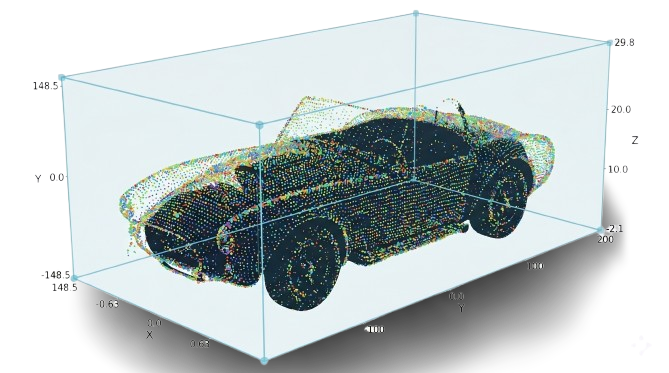
\includegraphics[width=0.72\textwidth]{images/methodology/box_bezier.png}
    \caption{Cube-mode initialization for a segmented object (classic car): COLMAP seed points (colored by SfM RGB) lie inside the object AABB $[\mathbf{b}_{\min},\mathbf{b}_{\max}]$ (semi-transparent box). The six faces of this box host the shared B\'ezier control lattice; $k\times k$ cubic patches per face are anchored to the lattice vertices merged at edges and corners.}
    \label{fig:bezier_cube_box}
\end{figure}

Neither mode implements a closed volumetric shell (no inner surface $S_{\mathrm{in}}$ or thickness layers). Empirically, cube mode with outlier filtering and FgBg losses gave the most regular exported meshes on both objects (Section~\ref{subsec:results_best_quant}), while open mode with FPS and outliers remained competitive on some Chamfer curves (e.g.\ pizza, Figure~\ref{fig:pizza_best_chamfer_bid}). Open initialization may be worth trying when seeds are fragmented or strongly curved locally; cube initialization is a strong default when a coherent six-face lattice is acceptable.

\subsection{B\'ezier Surface Parameterization}
\label{subsec:bezier_textures}

Beyond geometry, each surface patch $s$ can carry a learnable \textbf{texture grid}
\[
\mathbf{T}_s \in \mathbb{R}^{T\times T\times 4},
\qquad T=\texttt{bezier\_texture\_size}\ \ (\text{default }8),
\]
stored as \texttt{patch\_textures} and initialized uniformly in $[0,0.5]$ before sigmoid. For every Gaussian tied to patch $s$ at indices $(u_i,v_j)$ on the $N_u\times N_v$ sampling grid, texture coordinates are obtained by nearest indexing:
\begin{equation}
t_u = \mathrm{round}\!\left(u_i\,\frac{T-1}{N_u-1}\right),\qquad
t_v = \mathrm{round}\!\left(v_j\,\frac{T-1}{N_v-1}\right),
\label{eq:texture_index}
\end{equation}
and the pre-activation vector $\boldsymbol{\tau}=\mathbf{T}_s[t_u,t_v]\in\mathbb{R}^4$ is mapped through $\sigma(\cdot)$ (sigmoid) to RGBA in $[0,1]^4$. During \texttt{get\_outputs}, these values \emph{override} the static spherical-harmonic color and the stored opacity logit for that Gaussian for the current forward pass (Listing~\ref{lst:texture_override}).

\paragraph{In other words.}
Per patch, one defines a $T\times T$ grid of learnable color tiles (RGBA) and an $N_u\times N_v$ grid of Gaussians on the same surface. Each Gaussian keeps fixed indices $(s,i,j)$ (patch id and cell on the sampling lattice). At render time, $(i,j)$ is mapped to a tile $(t_u,t_v)$ via Eq.~\eqref{eq:texture_index}; that tile sets the splat's color and opacity for the forward pass. Under \textbf{code defaults} ($T{=}8$, $N_u{=}N_v{=}20$), $T^2{=}64$ tiles serve $N_u N_v{=}400$ Gaussians, so many splats share one tile. In \textbf{all B\'ezier runs reported in Chapter~\ref{chap:results}}, we instead set $T=N_u=N_v$ (typically $30$), giving a one-to-one assignment $t_u{=}i$, $t_v{=}j$ and one learnable RGBA tile per Gaussian on each patch; other hyperparameters (patch count, $\rho$, cube vs.\ open) vary by ablation, but this coupling was kept fixed so appearance resolution matches the sampling lattice.

\begin{lstlisting}[caption={Texture lookup in \texttt{get\_outputs} (open/cube mode).},label={lst:texture_override}]
tu = (uu * (T_tex - 1) / max(1, Nu - 1)).long()
tv = (vv * (T_tex - 1) / max(1, Nv - 1)).long()
rgba_01 = torch.sigmoid(patch_textures[pp, tu, tv])  # (N, 4)
features_dc = RGB2SH(rgba_01[:, :3])
opacities = torch.logit(rgba_01[:, 3:4].clamp(1e-6, 1-1e-6))
\end{lstlisting}

Higher-order SH bands are zeroed so view-dependent effects on the object surface are carried by the texture grid (and by joint motion of control points), not by per-Gaussian SH rest coefficients.

\subsection{Gaussian Parameter Initialization from B\'ezier Surfaces}
\label{subsec:gaussian_init}

Each sample $(s,i,j)$ on the uniform $(u,v)$ grid defines one 3D Gaussian primitive. Following Section~2.3.4, its learnable state is
\[
\boldsymbol{\Theta}_{s,i,j}=
\bigl\{
\boldsymbol{\mu}_{s,i,j},\,
\mathbf{s}_{s,i,j},\,
\mathbf{q}_{s,i,j},\,
o_{s,i,j},\,
\mathbf{f}_{s,i,j}
\bigr\},
\]
where $\boldsymbol{\mu}$ is the mean, $\mathbf{s}\in\mathbb{R}^3$ the \emph{log-scale} vector stored in the optimizer, $\mathbf{q}\in\mathbb{R}^4$ the unit quaternion (xyzw convention for \texttt{gsplat}), $o$ the opacity after sigmoid, and $\mathbf{f}$ the appearance coefficients (spherical harmonics or logits). Initialization is deterministic given control points $\{\mathbf{p}_{a,b}\}$ and configuration $(N_u,N_v,\rho,\alpha)$; index buffers \texttt{bezier\_open\_patch\_idx}, \texttt{bezier\_open\_u\_idx}, \texttt{bezier\_open\_v\_idx} record which $(s,i,j)$ each Gaussian represents for the lifetime of training.

\subsubsection{Mean positions}
\label{subsubsec:init_means}

Let $\mathbf{S}_s(u,v)$ be the $4\times 4$ B\'ezier patch for surface $s$. Discrete parameters $u_i=i/(N_u-1)$, $v_j=j/(N_v-1)$ yield sample positions
\begin{equation}
\boldsymbol{\mu}_{s,i,j}=\mathbf{S}_s(u_i,v_j)
=\sum_{a=0}^{3}\sum_{b=0}^{3} B_a^{3}(u_i)\,B_b^{3}(v_j)\,\mathbf{p}_{s,a,b},
\label{eq:gaussian_mean_bezier}
\end{equation}
with Bernstein polynomials $B_k^{3}$ as in Section~2.5.2. Stacking all patches gives $N_{\mathrm{g}}=S\cdot N_u\cdot N_v$ means. In \textbf{open/cube training}, $\boldsymbol{\mu}$ is \emph{recomputed} from the current control nets every forward pass via \texttt{\_bezier\_open\_resample\_means\_scales}, so gradients on rendering losses update $\mathbf{p}_{a,b}$ even though a \texttt{means} parameter tensor exists from init.

\subsubsection{Local tangent frame and quaternion}
\label{subsubsec:init_quat}

Let $\mathbf{X}_s\in\mathbb{R}^{N_u\times N_v\times 3}$ be the sampled grid for patch $s$. Discrete tangents use central differences in the interior and one-sided stencils on borders:
\begin{align}
\partial_u \mathbf{X}_{s,i,j} &\approx
\begin{cases}
\mathbf{X}_{s,i+1,j}-\mathbf{X}_{s,i-1,j} & 1\le i\le N_u-2,\\
\mathbf{X}_{s,1,j}-\mathbf{X}_{s,0,j} & i=0,\\
\mathbf{X}_{s,N_u-1,j}-\mathbf{X}_{s,N_u-2,j} & i=N_u-1,
\end{cases}
\label{eq:fd_u}\\
\partial_v \mathbf{X}_{s,i,j} &\approx
\text{(analogous along $j$)}.
\label{eq:fd_v}
\end{align}
Unit vectors $\mathbf{t}_u=\partial_u\mathbf{X}/\|\partial_u\mathbf{X}\|$, $\mathbf{t}_v=\partial_v\mathbf{X}/\|\partial_v\mathbf{X}\|$, and normal $\mathbf{n}=(\mathbf{t}_u\times\mathbf{t}_v)/\|\mathbf{t}_u\times\mathbf{t}_v\|$ are re-orthogonalized ($\mathbf{t}_v\leftarrow \mathbf{n}\times\mathbf{t}_u$) to form a right-handed frame. The rotation matrix $\mathbf{R}_{s,i,j}=[\mathbf{t}_u\;\mathbf{t}_v\;\mathbf{n}]\in SO(3)$ is converted to a quaternion $\mathbf{q}_{s,i,j}$ using COLMAP's \code{rotmat2qvec} and a wxyz$\rightarrow$xyzw reordering to match \code{gsplat}.

In the implementation, $\mathbf{q}_{s,i,j}$ is stored once at initialization in \code{gauss\_params["quats"]}; it is \textbf{not} refreshed when control points move during training (only $\boldsymbol{\mu}$ and $\mathbf{s}$ are resampled from the deformed surface). The initial frame therefore encodes the surface orientation at step zero.

\subsubsection{Anisotropic scales (log-space)}
\label{subsubsec:init_scales}

Gaussian covariance is modeled as $\boldsymbol{\Sigma}=\mathbf{R}\,\mathrm{diag}(\sigma_u^2,\sigma_v^2,\sigma_n^2)\,\mathbf{R}^\top$ (Section~2.3.4). Axis lengths are tied to the sampling grid and hyperparameters $\rho>0$, $\alpha>0$:
\begin{align}
\sigma_{u,s,i,j} &= \frac{\bigl\|\mathbf{X}_{s,i+1,j}-\mathbf{X}_{s,i,j}\bigr\|}{\rho}, \\
\sigma_{v,s,i,j} &= \frac{\bigl\|\mathbf{X}_{s,i,j+1}-\mathbf{X}_{s,i,j}\bigr\|}{\rho}, \\
\sigma_{n,s,i,j} &= \frac{\alpha}{\rho},
\label{eq:gaussian_scales}
\end{align}
with $\sigma_{u}$ at $i=N_u-1$ (and $\sigma_v$ at $j=N_v-1$) copied from the previous sample. The optimizer stores
\begin{equation}
\mathbf{s}_{s,i,j}=\log\bigl(\max(\boldsymbol{\sigma}_{s,i,j},\varepsilon)\bigr)\in\mathbb{R}^3,
\qquad
\boldsymbol{\sigma}_{s,i,j}=(\sigma_u,\sigma_v,\sigma_n)^\top,
\label{eq:log_scales}
\end{equation}
and \texttt{gsplat} uses $\mathrm{diag}(\exp(\mathbf{s}))$ inside the ellipsoid (same log-scale convention as in Section~2.3.4, not an extra modeling choice).

\paragraph{Role of $\rho$ and $\alpha$.}
Both hyperparameters act on the \textbf{geometric extent} of each Gaussian in the patch frame, not on its color or opacity. Let $\Delta_u=\|\mathbf{X}_{s,i+1,j}-\mathbf{X}_{s,i,j}\|$ be the Euclidean spacing between consecutive $(u,v)$ samples after surface deformation (and $\Delta_v$ analogously along $v$).
\begin{itemize}
    \item $\rho$ (\texttt{bezier\_rho}) compares tangential semi-axes to that spacing: $\sigma_u\approx \Delta_u/\rho$ and $\sigma_v\approx \Delta_v/\rho$. A splat therefore occupies roughly a $1/\rho$ fraction of the distance to its neighbor along each tangent. \textbf{Larger $\rho$} yields thinner, more numerous overlapping ellipsoids on the lattice (finer tiling of the surface in the $(u,v)$ plane); \textbf{smaller $\rho$} yields wider footprints that can over-blur detail or leave gaps if opacity is low. Because $\sigma_n=\alpha/\rho$, increasing $\rho$ also thins the shell along $\mathbf{n}$ unless $\alpha$ is raised.
    \item $\alpha$ (\texttt{bezier\_alpha}) sets only the normal semi-axis $\sigma_n=\alpha/\rho$, i.e.\ how thick the initial shell is \emph{perpendicular} to the surface. It does not depend on $\Delta_u,\Delta_v$: two samples on a stretched patch keep the same $\sigma_n$ until $\rho$ or $\alpha$ change. \textbf{Larger $\alpha$} makes each Gaussian more volumetric (less pancake-like); \textbf{smaller $\alpha$} keeps splats as thin sheets hugging $\mathbf{S}(u,v)$, which matches the B\'ezier-surface prior but offers less margin to represent offset geometry or slight misalignment between surface and true object.
\end{itemize}
In open/cube mode these formulas are reapplied every forward pass, so $(\rho,\alpha)$ remain the main levers on ellipsoid shape while control points move; quaternions are fixed at initialization (Section~\ref{subsubsec:init_quat}), so $\sigma_u,\sigma_v,\sigma_n$ always refer to the same local axes $\mathbf{t}_u,\mathbf{t}_v,\mathbf{n}$.

During training (open/cube), $\mathbf{s}$ is recomputed from the \emph{current} $\mathbf{X}$ via Eq.~\eqref{eq:gaussian_scales} (Listing~\ref{lst:open_resample_scales}).

\begin{lstlisting}[caption={Log-scale recomputation in \code{\_bezier\_open\_resample\_means\_scales}.},label={lst:open_resample_scales}]
du = X[:, 1:, :, :] - X[:, :-1, :, :]
sigma_u = ||du|| / rho   # pad last row
sigma_n = alpha / rho
scales_log = log(stack([sigma_u, sigma_v, sigma_n], dim=-1))
\end{lstlisting}

\subsubsection{Opacity}
\label{subsubsec:init_opacity}

Opacity is parameterized as $o=\sigma(\eta)$ with learnable logit $\eta$. At B\'ezier initialization all Gaussians share
\begin{equation}
\eta_{s,i,j}=\mathrm{logit}(0.1)=\log\frac{0.1}{0.9},
\label{eq:init_opacity_logit}
\end{equation}
i.e.\ initial visible opacity $o\approx 0.1$. When \texttt{patch\_textures} are enabled, $\eta$ is replaced at each forward by $\mathrm{logit}(\alpha_{s,i,j})$ where $\alpha_{s,i,j}$ is the sigmoid of the texture's fourth channel (Section~\ref{subsec:bezier_textures}).

\subsubsection{Summary of stored tensors}
\label{subsubsec:init_summary}

Table~\ref{tab:gaussian_init_bezier} lists the mapping from mathematical quantities to \code{SplatfactoModel} fields after B\'ezier init.

\begin{table}[htbp]
\centering
\footnotesize
\caption{B\'ezier-mode Gaussian initialization (open/cube). ``Resampled'' = recomputed each forward from current control points.}
\label{tab:gaussian_init_bezier}
\begin{tabularx}{\linewidth}{@{}l l >{\raggedright\arraybackslash}X >{\raggedright\arraybackslash}X@{}}
\toprule
Quantity & Symbol & Tensor / buffer & Updated during training \\
\midrule
Mean & $\boldsymbol{\mu}$ & \code{means} (then resampled) & Resampled from CP \\
Log-scale & $\mathbf{s}$ & \code{scales} (then resampled) & Resampled from CP \\
Quaternion & $\mathbf{q}$ & \code{quats} & Fixed after init \\
Opacity logit & $\eta$ & \code{opacities} & Learned; or from texture \\
SH coefficients & $\mathbf{f}$ & \code{features\_dc}, \code{features\_rest} & Learned; or from texture \\
Patch indices & $(s,i,j)$ & \code{bezier\_open\_*\_idx} & Fixed buffers \\
Control points & $\mathbf{p}_{a,b}$ & \code{bezier\_open\_cp} / \code{bezier\_cube\_shared\_cp} & Optimized \\
Texture & $\mathbf{T}_s$ & \code{patch\_textures} & Optimized \\
\bottomrule
\end{tabularx}
\end{table}

\paragraph{Contrast with classical COLMAP initialization.}
If B\'ezier init is disabled, means are COLMAP points, scales are $\log(\bar{d})$ with $\bar{d}$ the mean distance to three nearest neighbors (isotropic), quaternions are random unit quaternions, and colors come from per-point SfM RGB via \texttt{RGB2SH}. B\'ezier initialization replaces the unstructured cloud with a structured $N_u\times N_v$ lattice on $\mathbf{S}(u,v)$, oriented anisotropic covariances aligned to $\mathbf{t}_u,\mathbf{t}_v,\mathbf{n}$, and fixed semantic indices per Gaussian.

\begin{lstlisting}[caption={Classical COLMAP scale init (fallback path, \filepath{splatfacto.py}).},label={lst:classic_scale}]
distances, _ = k_nearest_sklearn(means, k=3)
avg_dist = distances.mean(dim=-1).clamp(min=1e-6)
scales = torch.nn.Parameter(torch.log(avg_dist.repeat(1, 3)))  # isotropic log-scale
\end{lstlisting}

\subsection{Integration into the Splatting and Training Pipeline}
\label{subsec:bezier_pipeline}

B\'ezier-mode Splatfacto reuses the standard \code{gsplat} rasterizer and Nerfstudio trainer; the difference is \emph{which} tensors are optimized and how geometry is refreshed each step. Training still follows the loop of Chapter~\ref{chap:tools}: sample a full-frame camera, then \code{get\_outputs}, rasterization, \code{get\_loss\_dict}, backward pass, and optimizer step.

\subsubsection{Parameter registration and optimizer groups}
\label{subsubsec:bezier_optimizer}

Gaussian attributes live in \code{gauss\_params}. In open/cube B\'ezier mode, \code{get\_gaussian\_param\_groups} \emph{rebinds} the optimizer:
\begin{itemize}
    \item \textbf{Geometry:} \code{bezier\_open\_cp} $(S,4,4,3)$ or \code{bezier\_cube\_shared\_cp} $(N_{\mathrm{unique}},3)$ is registered under the \code{means} group (replacing free 3D positions). The classical \code{scales} group is \emph{dropped} from the optimizer (Listing~\ref{lst:param_groups}).
    \item \textbf{Appearance:} optional \code{patch\_textures} $(S,T,T,4)$ in group \code{patch\_textures} (lr $2.5\times 10^{-3}$).
    \item \textbf{Remaining splats:} \code{quats}, \code{features\_dc/rest}, \code{opacities} keep their classical groups unless textures override color/opacity in the forward pass (then gradients flow into $\mathbf{T}_s$ instead).
    \item \textbf{Cameras / bilateral:} unchanged (\code{camera\_opt}, \code{bilateral\_grid} if enabled).
\end{itemize}

\paragraph{Why \texttt{scales} are omitted from the optimizer.}
In standard 3DGS, \code{gauss\_params["scales"]} is a learnable tensor: Adam updates it and the rasterizer reads $\exp(\mathbf{s})$ directly. In open/cube B\'ezier mode this is \emph{not} the case: each forward pass recomputes $\boldsymbol{\mu}_{s,i,j}$ and $\mathbf{s}_{s,i,j}=\log\boldsymbol{\sigma}_{s,i,j}$ from the \emph{current} control net via Eq.~\eqref{eq:reparam_chain} and \eqref{eq:gaussian_scales} (\texttt{\_bezier\_open\_resample\_means\_scales}), then passes those tensors to \texttt{gsplat}. Ellipsoid sizes therefore follow automatically from surface sampling density and $(\rho,\alpha)$; they are still used in rendering, but they are not independent degrees of freedom. Keeping \code{scales} in the optimizer would apply updates that the next forward overwrites, while the loss gradients on $\mathbf{s}$ already reach the control points through $\partial\mathbf{s}/\partial\mathbf{p}$. What is learned is the surface geometry (and optionally \texttt{patch\_textures}), not a separate log-scale vector per Gaussian (e.g.\ $N_u N_v$ scalars per patch).

Default learning rates in \texttt{method\_configs.py} mirror 3DGS: control-net tensors use the same exponential decay as means ($1.6\times 10^{-4}\rightarrow 1.6\times 10^{-6}$ over 30k steps). Listing~\ref{lst:param_groups} shows the registration logic.

\begin{lstlisting}[caption={Open/cube B\'ezier parameter groups (\filepath{splatfacto.py}).},label={lst:param_groups}]
if hasattr(self, "bezier_open_cp"):
    gps["means"] = [self.bezier_open_cp]   # CP tensor uses the "means" slot
    gps.pop("scales", None)
    if hasattr(self, "patch_textures"):
        gps["patch_textures"] = [self.patch_textures]
\end{lstlisting}

\paragraph{Adaptive densification disabled.}
Classical Splatfacto clones/splits/prunes Gaussians from view-space gradient statistics. In B\'ezier open/cube mode this is turned off (\code{skip\_densify=True} in \code{get\_outputs}), because the Gaussian count and $(s,i,j)$ indices are fixed by the $(N_u,N_v)$ lattice on each patch. All geometric degrees of freedom are in the control nets (and textures), not in the number of primitives.

\subsection{Gradient propagation to control points}
\label{subsec:bezier_gradients}

Differentiable rasterization \cite{kerbl2023gaussian} back-propagates $\partial\mathcal{L}/\partial\mathbf{C}$ to per-Gaussian color and opacity, then through projection to 3D means, covariances, and opacities. Figure~\ref{fig:3dgs_grad_graph} reproduces the standard 3DGS backward graph (screen-space Gaussian $G'$, projection $P$, covariance $\boldsymbol{\Sigma}=RSS^\top R^\top$, sigmoid opacity).

\begin{figure}[H]
    \centering
    \resizebox{0.98\textwidth}{!}{%
    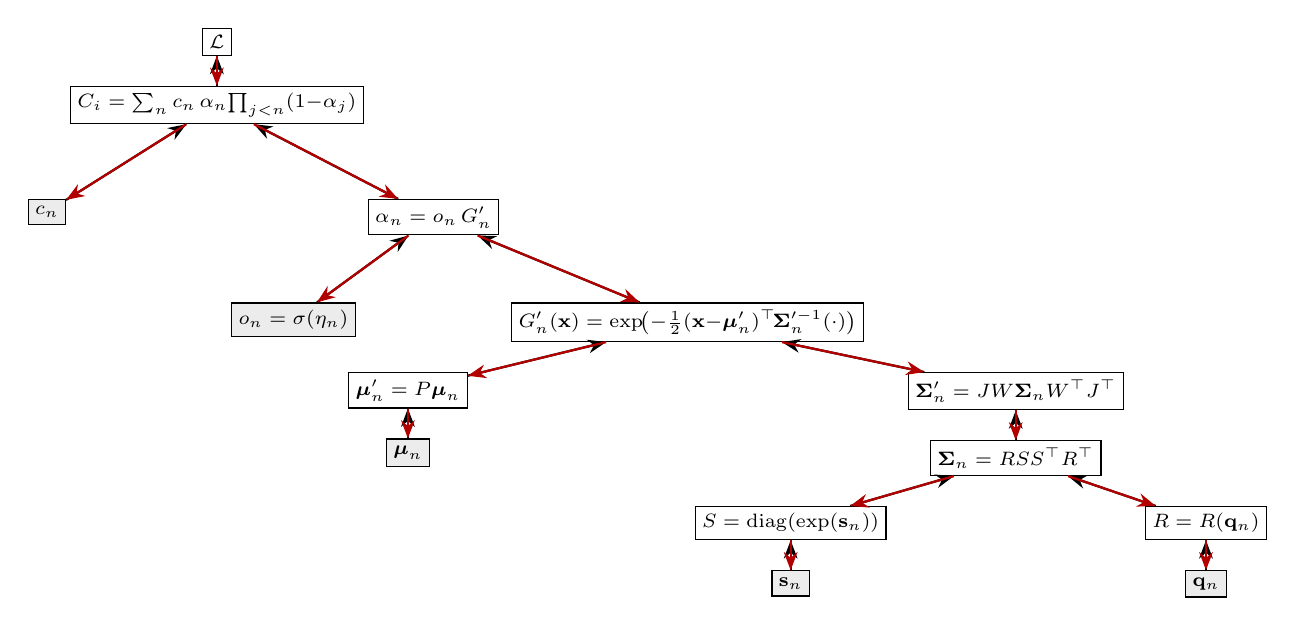
\begin{tikzpicture}[
        node distance=0.38cm and 0.55cm,
        every node/.style={rectangle, draw, align=center, font=\scriptsize, inner sep=2.5pt},
        leaf/.style={fill=gray!15},
        grad/.style={-{Stealth}, red!70!black, thick},
        fwd/.style={-{Stealth}, thick},
    ]
        \node (L) {$\mathcal{L}$};
        \node[below=of L] (Ci) {$C_i=\sum_n c_n\,\alpha_n\!\prod_{j<n}(1{-}\alpha_j)$};
        \node[below left=0.95cm and 0.05cm of Ci, leaf] (cn) {$c_n$};
        \node[below right=0.95cm and 0.05cm of Ci] (an) {$\alpha_n=o_n\,G'_n$};
        \node[below left=0.85cm and 0.15cm of an, leaf] (on) {$o_n=\sigma(\eta_n)$};
        \node[below right=0.85cm and 0.15cm of an] (Gn) {$G'_n(\mathbf{x})=\exp\!\bigl(-\tfrac12(\mathbf{x}{-}\boldsymbol{\mu}'_n)^\top\!\boldsymbol{\Sigma}_n'^{-1}(\cdot)\bigr)$};
        \node[below left=of Gn] (mup) {$\boldsymbol{\mu}'_n=P\boldsymbol{\mu}_n$};
        \node[below=of mup, leaf] (mu) {$\boldsymbol{\mu}_n$};
        \node[below right=of Gn] (Sp) {$\boldsymbol{\Sigma}'_n=J W\boldsymbol{\Sigma}_n W^\top J^\top$};
        \node[below=of Sp] (Sig) {$\boldsymbol{\Sigma}_n=R S S^\top R^\top$};
        \node[below left=of Sig] (sexp) {$S=\mathrm{diag}(\exp(\mathbf{s}_n))$};
        \node[below=of sexp, leaf] (sn) {$\mathbf{s}_n$};
        \node[below right=of Sig] (qrot) {$R=R(\mathbf{q}_n)$};
        \node[below=of qrot, leaf] (qn) {$\mathbf{q}_n$};
        % forward (parameter $\rightarrow$ render)
        \draw[fwd] (mu) -- (mup);
        \draw[fwd] (sn) -- (sexp);
        \draw[fwd] (sexp) -- (Sig);
        \draw[fwd] (qn) -- (qrot);
        \draw[fwd] (qrot) -- (Sig);
        \draw[fwd] (Sig) -- (Sp);
        \draw[fwd] (mup) -- (Gn);
        \draw[fwd] (Sp) -- (Gn);
        \draw[fwd] (on) -- (an);
        \draw[fwd] (Gn) -- (an);
        \draw[fwd] (cn) -- (Ci);
        \draw[fwd] (an) -- (Ci);
        \draw[fwd] (Ci) -- (L);
        % backward (loss $\rightarrow$ parameters)
        \draw[grad] (L) -- (Ci);
        \draw[grad] (Ci) -- (cn);
        \draw[grad] (Ci) -- (an);
        \draw[grad] (an) -- (on);
        \draw[grad] (an) -- (Gn);
        \draw[grad] (Gn) -- (mup);
        \draw[grad] (Gn) -- (Sp);
        \draw[grad] (mup) -- (mu);
        \draw[grad] (Sp) -- (Sig);
        \draw[grad] (Sig) -- (sexp);
        \draw[grad] (Sig) -- (qrot);
        \draw[grad] (sexp) -- (sn);
        \draw[grad] (qrot) -- (qn);
    \end{tikzpicture}%
    }
    \caption{Backward pass in 3D Gaussian Splatting (adapted from \cite{kerbl2023gaussian}): loss $\mathcal{L}$ $\rightarrow$ pixel color $C_i$ $\rightarrow$ opacities $\alpha_n$ and colors $c_n$ $\rightarrow$ projected 2D Gaussian $G'_n$ $\rightarrow$ 3D mean $\boldsymbol{\mu}_n$, scales $\mathbf{s}_n$, quaternion $\mathbf{q}_n$. Red arrows indicate gradient flow; black arrows the forward evaluation chain.}
    \label{fig:3dgs_grad_graph}
\end{figure}

\paragraph{B\'ezier extension of the chain.}
In open/cube mode the \emph{effective} 3D position and covariance used at render time are functional outputs of the control net, not the stored \code{gauss\_params["means"]} tensor. Each training step executes
\begin{align}
\mathbf{X}_s &= \mathrm{SampleBezier}\bigl(\{\mathbf{p}_{s,a,b}\}\bigr), \\
\boldsymbol{\mu}_{s,i,j} &= \mathbf{X}_s(u_i,v_j), \\
\mathbf{s}_{s,i,j} &= \log\boldsymbol{\sigma}(\mathbf{X}_s,\rho,\alpha),
\label{eq:reparam_chain}
\end{align}
before calling \code{gsplat.rasterization}. Therefore, by the chain rule,
\begin{equation}
\frac{\partial\mathcal{L}}{\partial \mathbf{p}_{s,a,b}}
=
\sum_{i,j}
\left(
\frac{\partial\mathcal{L}}{\partial\boldsymbol{\mu}_{s,i,j}}
\frac{\partial\boldsymbol{\mu}_{s,i,j}}{\partial \mathbf{p}_{s,a,b}}
+
\frac{\partial\mathcal{L}}{\partial\mathbf{s}_{s,i,j}}
\frac{\partial\mathbf{s}_{s,i,j}}{\partial \mathbf{p}_{s,a,b}}
\right),
\label{eq:grad_cp_chain}
\end{equation}
where $\partial\boldsymbol{\mu}/\partial\mathbf{p}$ comes from Bernstein blending (Eq.~\eqref{eq:gaussian_mean_bezier}) and $\partial\mathbf{s}/\partial\mathbf{p}$ from finite-difference spacing (Eq.~\eqref{eq:gaussian_scales}). Quaternions $\mathbf{q}_{s,i,j}$ are fixed after initialization in the current implementation, so $\partial\mathcal{L}/\partial\mathbf{q}$ does not feed back into $\mathbf{p}$ unless orientations are recomputed each forward.

If \texttt{patch\_textures} are active, color and opacity at sample $(s,i,j)$ satisfy
$c_n=\mathrm{SH2RGB}(\mathrm{RGB2SH}(\sigma(\mathbf{T}_s[t_u,t_v])_{0:3}))$ and $\eta_n=\mathrm{logit}(\sigma(\mathbf{T}_s)_{3})$, giving an additional branch $\partial\mathcal{L}/\partial\mathbf{T}_s$.

Figure~\ref{fig:bezier_grad_graph} summarizes the combined graph (classic splatting backbone + B\'ezier reparameterization).

\begin{figure}[H]
    \centering
    \resizebox{0.95\textwidth}{!}{%
    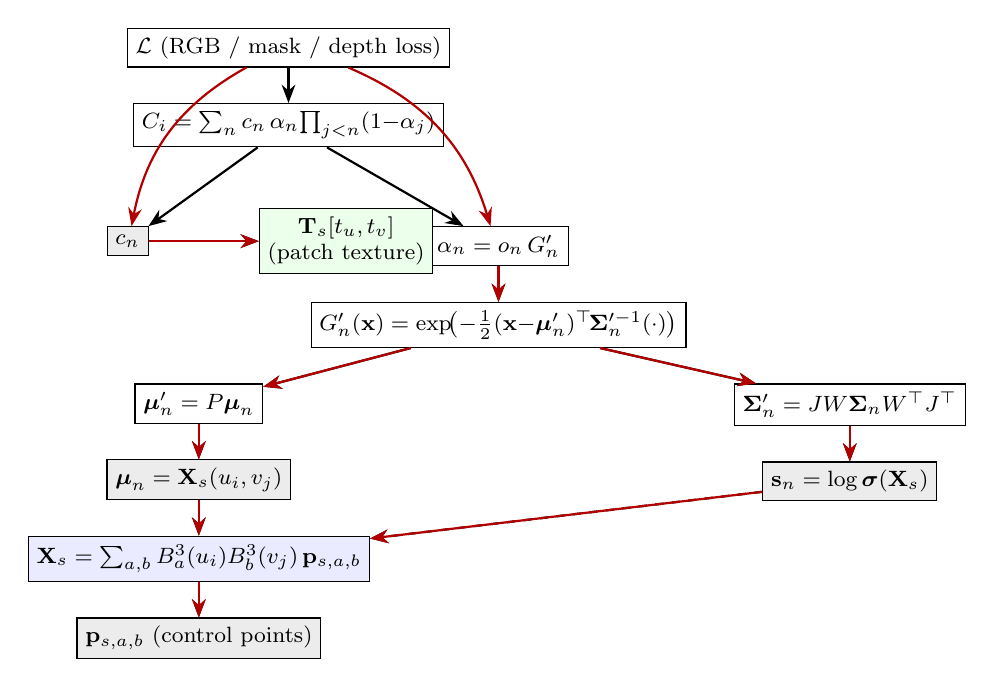
\begin{tikzpicture}[
        node distance=0.45cm and 0.6cm,
        every node/.style={rectangle, draw, align=center, font=\footnotesize, inner sep=3pt},
        leaf/.style={fill=gray!15},
        grad/.style={-{Stealth}, red!70!black, thick},
        fwd/.style={-{Stealth}, thick},
    ]
        \node (L) {$\mathcal{L}$ (RGB / mask / depth loss)};
        \node[below=of L] (Ci) {$C_i=\sum_n c_n\,\alpha_n\!\prod_{j<n}(1{-}\alpha_j)$};
        \node[below left=1.0cm and -0.2cm of Ci, leaf] (cn) {$c_n$};
        \node[below right=1.0cm and -0.2cm of Ci] (an) {$\alpha_n=o_n\,G'_n$};
        \node[below=of an] (Gn) {$G'_n(\mathbf{x})=\exp\!\bigl(-\tfrac12(\mathbf{x}{-}\boldsymbol{\mu}'_n)^\top\!\boldsymbol{\Sigma}_n'^{-1}(\cdot)\bigr)$};
        \node[below left=of Gn] (mup) {$\boldsymbol{\mu}'_n=P\boldsymbol{\mu}_n$};
        \node[below right=of Gn] (Sp) {$\boldsymbol{\Sigma}'_n=J W\boldsymbol{\Sigma}_n W^\top J^\top$};
        \node[below=of mup, leaf] (mu) {$\boldsymbol{\mu}_n=\mathbf{X}_s(u_i,v_j)$};
        \node[below=of mu, fill=blue!8] (X) {$\mathbf{X}_s=\sum_{a,b}B_a^{3}(u_i)B_b^{3}(v_j)\,\mathbf{p}_{s,a,b}$};
        \node[below=of X, leaf] (cp) {$\mathbf{p}_{s,a,b}$ (control points)};
        \node[below=of Sp, leaf] (sn) {$\mathbf{s}_n=\log\boldsymbol{\sigma}(\mathbf{X}_s)$};
        \node[right=1.4cm of cn, fill=green!8] (tex) {$\mathbf{T}_s[t_u,t_v]$\\(patch texture)};
        \draw[fwd] (L) -- (Ci);
        \draw[fwd] (Ci) -- (cn); \draw[fwd] (Ci) -- (an);
        \draw[fwd] (an) -- (Gn);
        \draw[fwd] (Gn) -- (mup); \draw[fwd] (Gn) -- (Sp);
        \draw[fwd] (mup) -- (mu); \draw[fwd] (mu) -- (X); \draw[fwd] (X) -- (cp);
        \draw[fwd] (Sp) -- (sn); \draw[fwd, dashed] (sn) -- (X);
        \draw[fwd, dashed] (cn) -- (tex);
        \draw[grad] (L) to[bend right=25] (cn);
        \draw[grad] (L) to[bend left=25] (an);
        \draw[grad] (an) -- (Gn);
        \draw[grad] (Gn) -- (mup); \draw[grad] (Gn) -- (Sp);
        \draw[grad] (mup) -- (mu); \draw[grad] (mu) -- (X);
        \draw[grad] (X) -- (cp);
        \draw[grad] (Sp) -- (sn);
        \draw[grad] (sn) -- (X);
        \draw[grad] (cn) -- (tex);
    \end{tikzpicture}%
    }
    \caption{Gradient flow in B\'ezier-mode Splatfacto: standard 3DGS splatting derivatives (top) plus reparameterization $\boldsymbol{\mu}_n,\mathbf{s}_n\leftarrow\mathbf{X}_s(\mathbf{p})$ (blue) and optional texture branch (green). Dashed forward links indicate resampled scales/colors tied to the same $\mathbf{X}_s$.}
    \label{fig:bezier_grad_graph}
\end{figure}

\paragraph{Implementation notes.}
\begin{itemize}
    \item \texttt{\_bezier\_open\_resample\_means\_scales} is called inside \texttt{get\_outputs} \emph{before} rasterization, so \texttt{gsplat} always sees $\boldsymbol{\mu},\mathbf{s}$ consistent with the current $\mathbf{p}$.
    \item Autograd must not use in-place writes on $\mathbf{X}_s$ when building $\boldsymbol{\sigma}$ (the code uses \texttt{torch.cat} rather than in-place assignment for this reason).
    \item Optional $\mathcal{L}_{\mathrm{CP}}=\lambda_{\mathrm{L2}}\|\mathbf{p}\|_2^2$ (\texttt{bezier\_open\_cp\_l2\_lambda}) adds a direct regularizer on control points in addition to the rendering loss.
\end{itemize}

\subsection{Regularization Strategy}
\label{subsec:bezier_regularization}

\subsubsection{Control Point $L_2$ Regularization}
\label{subsubsec:cp_l2}

An optional penalty
\begin{equation}
\mathcal{L}_{\mathrm{CP}}
=\lambda_{\mathrm{L2}}\,\frac{1}{|\mathcal{P}|}\sum_{s,a,b}\|\mathbf{p}_{s,a,b}\|_2^2,
\qquad
\lambda_{\mathrm{L2}}=\texttt{bezier\_open\_cp\_l2\_lambda},
\label{eq:cp_l2}
\end{equation}
is added to the total loss when $\lambda_{\mathrm{L2}}>0$ (\texttt{bezier\_open\_cp\_l2\_lambda}, default $0$). The intent is to limit excessive drift of control points away from their initialization while still allowing the rendering term to deform the surface.

In the experiments reported in Chapter~\ref{chap:results}, enabling $\mathcal{L}_{\mathrm{CP}}$ did not produce qualitative or metric differences that were clearly distinguishable from the baseline without regularization (same PSNR/SSIM and similar visual inspection). The term is therefore documented for completeness but was not used as a primary knob in the final B\'ezier configurations.

\begin{lstlisting}[caption={Optional CP $L_2$ term (\filepath{splatfacto.py}).},label={lst:cp_l2}]
if bezier_open_cp_l2_lambda != 0.0:
    loss_dict["bezier_cp_l2_loss"] = lambda_reg * (bezier_open_cp ** 2).mean()
\end{lstlisting}

\subsection{Mask-Based Supervision}
\label{subsec:mask_losses}

SAM~2 masks serve two distinct purposes in this pipeline. During \textbf{initialization} (Section~\ref{subsec:semantic_isolation}), they label COLMAP seed points and select which geometry enters B\'ezier fitting; all object-centric experiments in this thesis use that step. At \textbf{training} time, masks can additionally enter the loss: several ablation configurations in Chapter~\ref{chap:results} (names containing \texttt{FgBg}) load exported binary masks and optimize a decomposed foreground--background objective (Section~\ref{subsubsec:mask_combined}), while others keep the full-frame $\mathcal{L}_{\mathrm{rgb}}$ of Section~\ref{sec:baseline_3dgs} and rely on segmentation for initialization only.

Early B\'ezier trials used full-frame $\mathcal{L}_{\mathrm{rgb}}$ with masks at init alone. In open/cube mode, geometry is then optimized \emph{indirectly}: gradients on splatted Gaussians propagate to control nets through $\mathbf{S}(u,v)$. When a patch drifts outside the object region, for example because outlier seeds biased initialization, the global mean can still decrease while the surface projects mainly into background pixels and receives no signal aligned with the object of interest. The FgBg decomposition was introduced to correct this failure mode and was evaluated alongside full-frame runs throughout the ablation matrix (Section~\ref{sec:results_ablation}), not only in the final best configuration.

When masks are exported to the dataparser (\code{convert\_sam2\_labelmaps\_to\_binary\_masks}), each training batch may include \code{batch["mask"]} $M\in[0,1]^{H\times W\times 1}$ (resampled like RGB), with background $B=1-M$. Instead of a single mean over all pixels, the objective separates (i)~photometric fitting on foreground pixels $M$ and (ii)~opacity-based constraints on $B$ and $M$ under \texttt{mask\_bg\_target=emptiness} (Section~\ref{subsubsec:mask_bg}), weighted by $\lambda_{\mathrm{fg}}$, $\lambda_{\mathrm{bg}}$, and $\lambda_{\mathrm{sil}}$.

\subsubsection{Foreground photometric term}
\label{subsubsec:mask_fg}

Let $\hat{\mathbf{I}}$ and $\mathbf{I}_{\mathrm{gt}}$ be predicted and ground-truth RGB (before masking). With $\|\cdot\|_{p}$ denoting per-pixel $L_1$ ($p=1$) or $L_2$ ($p=2$, \texttt{mask\_loss\_norm}) error,
\begin{equation}
\mathcal{L}_{\mathrm{fg}}
=\frac{\sum_{x} M(x)\,\bigl\|\hat{\mathbf{I}}(x)-\mathbf{I}_{\mathrm{gt}}(x)\bigr\|_{p}}
{\sum_{x} M(x) + \varepsilon},
\qquad \varepsilon=10^{-6}.
\label{eq:mask_fg}
\end{equation}
Normalization by $\sum_x M(x)$ keeps the loss magnitude stable when the object occupies a small fraction of the image (important for centered objects such as the chair or car scenes). With $\lambda_{\mathrm{fg}}=1$ and $\lambda_{\mathrm{bg}}=\lambda_{\mathrm{sil}}=0$, Eq.~\eqref{eq:mask_combined} reduces to $\mathcal{L}_{\mathrm{mask}}=\mathcal{L}_{\mathrm{fg}}$: the same $L_1$ (or $L_2$) photometric error as the baseline, but averaged \emph{only over object pixels} rather than the full frame. Non-zero $\lambda_{\mathrm{bg}}$ or $\lambda_{\mathrm{sil}}$ add explicit background or silhouette terms on top of this object-only photometric core; many study runs (e.g.\ \texttt{CubeL1FgBgOut}) combine $\mathcal{L}_{\mathrm{fg}}$ with small background weights rather than object-only training.

For D-SSIM, both images are multiplied by $M$ before the SSIM windowing so only foreground pixels contribute:
$\mathbf{I}_{\mathrm{masked}}=\mathbf{I}\odot M$, $\hat{\mathbf{I}}_{\mathrm{masked}}=\hat{\mathbf{I}}\odot M$.

\subsubsection{Background terms}
\label{subsubsec:mask_bg}

The implementation also exposes RGB background modes \texttt{mask\_bg\_target}$\in\{\texttt{black},\texttt{gt}\}$ (penalize non-zero or ground-truth color outside $M$); they were not used in the reported experiments. All FgBg runs in Chapter~\ref{chap:results} instead set \texttt{mask\_bg\_target=emptiness}: background constraints act on \textbf{accumulated opacity} $A(x)\in[0,1]$ from the rasterizer (\code{outputs["accumulation"]}), not on RGB outside the mask. The background should be transparent and the object opaque:
\begin{align}
\mathcal{L}_{\mathrm{bg}}^{\mathrm{empty}}
&=\frac{\sum_{x} B(x)\,A(x)^2}{\sum_{x} B(x) + \varepsilon},
\label{eq:mask_bg_empty}\\
\mathcal{L}_{\mathrm{sil}}
&=\frac{\sum_{x} M(x)\,(1-A(x))^2}{\sum_{x} M(x) + \varepsilon}.
\label{eq:mask_sil}
\end{align}
$\mathcal{L}_{\mathrm{bg}}^{\mathrm{empty}}$ drives $A\to 0$ outside the object (no ``fog'' or floaters in background). $\mathcal{L}_{\mathrm{sil}}$ prevents the object from \emph{collapsing} to transparency inside the mask, which $\mathcal{L}_{\mathrm{bg}}^{\mathrm{empty}}$ alone would not forbid.

\subsubsection{Combined mask loss and full objective}
\label{subsubsec:mask_combined}

For \texttt{mask\_bg\_target=emptiness}, the decomposed $L_1$ (or $L_2$) part of the main loss is
\begin{equation}
\mathcal{L}_{\mathrm{mask}}
=\lambda_{\mathrm{fg}}\mathcal{L}_{\mathrm{fg}}
+\lambda_{\mathrm{bg}}\mathcal{L}_{\mathrm{bg}}^{\mathrm{empty}}
+\lambda_{\mathrm{sil}}\mathcal{L}_{\mathrm{sil}}.
\label{eq:mask_combined}
\end{equation}
Study runs typically set $\lambda_{\mathrm{fg}}=1.0$; $\lambda_{\mathrm{bg}}$ and $\lambda_{\mathrm{sil}}$ are often zero when only object-only photometric fitting is desired (Section~\ref{subsubsec:mask_fg}). Repository defaults are $\lambda_{\mathrm{fg}}=1.0$, $\lambda_{\mathrm{bg}}=0.2$, $\lambda_{\mathrm{sil}}=0.1$. For RGB training (\texttt{loss=rgb}),
\begin{equation}
\mathcal{L}
=(1-\lambda_{\mathrm{ssim}})\,\mathcal{L}_{\mathrm{mask}}
+\lambda_{\mathrm{ssim}}\,\mathcal{L}_{\mathrm{D\text{-}SSIM}},
\qquad \lambda_{\mathrm{ssim}}=\texttt{ssim\_lambda}=0.2.
\label{eq:mask_total_rgb}
\end{equation}
When \texttt{loss=depth}, $\mathcal{L}_{\mathrm{mask}}$ reduces to masked mean $|d^{\mathrm{exp}}-d_{\mathrm{DA3}}|$ (Eq.~\eqref{eq:mask_fg} applied to depth channels) and SSIM is omitted.

\begin{lstlisting}[caption={FG/BG decomposed loss, emptiness mode (\filepath{splatfacto.py}, RGB; branch used in reported runs).},label={lst:mask_loss}]
M, B = mask, 1.0 - mask
L_fg = (abs(pred - gt) * M).sum() / (M.sum() + eps)
accum = outputs["accumulation"]
L_bg = (B * accum**2).sum() / (B.sum() + eps)
L_sil = (M * (1.0 - accum)**2).sum() / (M.sum() + eps)
Ll1 = mask_lambda_fg * L_fg + mask_lambda_bg * L_bg + mask_lambda_sil * L_sil
main_loss = (1 - ssim_lambda) * Ll1 + ssim_lambda * (1 - SSIM(gt*M, pred*M))
\end{lstlisting}

\paragraph{When the masked objective is active.}
The FG/BG decomposition is used only if \texttt{"mask" in batch}; otherwise training keeps the unmasked $\mathcal{L}_{\mathrm{rgb}}$ (or depth loss) even in B\'ezier mode. Mask files under \filepath{masks/} (and optional \filepath{masks\_4/} for downscaled training) must therefore be exported \emph{and} loaded by the dataparser for the regularizer to take effect. The same implementation also supports classical Gaussian training on the full cloud; in this thesis, the masked loss was evaluated mainly on object-centric B\'ezier scenes after the unconstrained runs showed surface drift and background leakage.


\chapter{Results}
\label{chap:results}

\section{Experimental Setup}
\label{sec:results_setup}

\subsection{Evaluation Metrics}
\label{subsec:eval_metrics}

Training and exported meshes were monitored in \textbf{TensorBoard}. For geometry, each run logs \textbf{unidirectional} and \textbf{bidirectional Chamfer distance} between a reference point cloud (COLMAP object seeds or a held-out dense sample) and the B\'ezier mesh sampled at export resolution. Unidirectional Chamfer measures the mean nearest-neighbor distance from prediction to reference; bidirectional Chamfer averages both directions and penalizes missing geometry as well as excess surface. Lower values indicate closer alignment with the reference. Control-point stability is analyzed through the logged gradient norm on B\'ezier parameters (\texttt{bezier\_open\_cp} or \texttt{bezier\_cube\_shared\_cp}), reported as smoothed TensorBoard curves over 30k iterations.

\subsection{Test Scenes}
\label{subsec:test_scenes}

Results focus on two object-centric captures used throughout the B\'ezier experiments: a \textbf{pizza} (compact, roughly convex) and a \textbf{parking meter} (elongated structure, more challenging occlusion and background clutter). Both scenes use Grounded SAM~2 masks for initialization. Reported configurations differ by loss: \texttt{Open/Cube L1} use full-frame photometric $L_1$; names with \texttt{FgBg} additionally apply the decomposed mask objective of Section~\ref{subsec:mask_losses} during training.

\subsection{B\'ezier Hyperparameters in the Study}
\label{subsec:bezier_study_hparams}

Unless an ablation name states otherwise, reported B\'ezier trainings set \texttt{bezier\_texture\_size}$=N_u=N_v$ (commonly $30$), so each of the $N_u N_v$ Gaussians on a patch reads a distinct texture tile (Section~\ref{subsec:bezier_textures}). This differs from the repository defaults ($T{=}8$, $N_u{=}N_v{=}20$), where tiles are shared across groups of splats. Open-mode ablations additionally use \texttt{bezier\_num\_patches\_per\_class} on the order of $30$ with \texttt{bezier\_center\_sampling} \texttt{fps} or \texttt{random}; cube-mode runs use the AABB lattice ($6k^2$ face patches) with the same $N_u,N_v,T$ coupling for per-Gaussian textures. Values such as \texttt{bezier\_rho} (e.g.\ $20$--$100$) and mask-loss weights are varied between runs and are identified by the configuration labels in Section~\ref{sec:results_ablation}.

\section{Best Result: B\'ezier Structural Model, Cube Mode, Outlier Management}
\label{sec:results_best_cube_outliers}

The reference configuration is \textbf{Cube L1 FgBg Out}: cube-mode patches on the object AABB, full-frame $L_1$ photometric loss decomposed into foreground and background terms, and $k$-NN outlier rejection before patch fitting (Section~\ref{subsec:knn_outlier}). Among all ablations, it offers the best trade-off between mesh fidelity, training stability, and visual cleanliness on both test scenes.

\subsection{Qualitative Analysis}
\label{subsec:results_best_qual}

Figure~\ref{fig:best_pizza_qual} summarizes the pizza scene: multi-view RGB renders, predicted depth maps, and the exported cube-mode mesh. The surface stays inside the segmented region, with coherent patch layout and no large detached sheets; the background remains dark in RGB, consistent with FgBg supervision. Figure~\ref{fig:best_parking_qual} reports the same configuration on the parking meter, where the elongated body and coin head are captured without the severe floaters seen in unconstrained baselines (Section~\ref{sec:results_baseline_compare}).

\begin{figure}[H]
    \centering
    \resabl{images/conclusion/pizza_ablationstudy_cubeL1FgBg_outliers.png}
    \caption{Pizza scene, Cube L1 FgBg Out.: multi-view RGB renders (left), predicted depth maps (center), and exported mesh (right).}
    \label{fig:best_pizza_qual}
\end{figure}

\begin{figure}[H]
    \centering
    \resabl{images/conclusion/parkingmetere_ablationstudy_cubel1fgbg_outliers.png}
    \caption{Parking meter, Cube L1 FgBg Out.: multi-view RGB renders (left), predicted depth maps (center), and exported mesh (right).}
    \label{fig:best_parking_qual}
\end{figure}

\subsection{Quantitative Evaluation}
\label{subsec:results_best_quant}

On the pizza scene, unidirectional Chamfer for cube-mode runs without outlier management remains an order of magnitude higher than with outliers (Figure~\ref{fig:pizza_cube_chamfer_uni}): \texttt{CubeL1FgBgOut} plateaus near $0.18$ while \texttt{CubeL1} and \texttt{CubeL1FgBg} stay above $21$. Bidirectional Chamfer on the same scene (Figure~\ref{fig:pizza_cube_chamfer_bid}) shows the same separation. Figure~\ref{fig:pizza_best_chamfer_bid} compares the strongest outlier-aware variants across open and cube modes; \texttt{CubeL1FgBgOut} reaches a low stable bidirectional error, confirming the best-result choice. The parking-meter scene exhibits the same trend (Figures~\ref{fig:parking_cube_chamfer_uni}--\ref{fig:parking_best_chamfer_bid}), with outlier-managed runs converging to substantially smaller Chamfer values.

\begin{figure}[H]
    \centering
    \resplot{images/conclusion/pizza_cube_chamfer_unid.png}
    \caption{Pizza: unidirectional Chamfer distance (cube-mode ablations).}
    \label{fig:pizza_cube_chamfer_uni}
\end{figure}

\begin{figure}[H]
    \centering
    \resplot{images/conclusion/pizza_cube_chamfer_bid.png}
    \caption{Pizza: bidirectional Chamfer distance (cube-mode ablations).}
    \label{fig:pizza_cube_chamfer_bid}
\end{figure}

\begin{figure}[H]
    \centering
    \resplot{images/conclusion/pizza_best_chamfer_bid.png}
    \caption{Pizza: bidirectional Chamfer for the best outlier-managed open/cube variants.}
    \label{fig:pizza_best_chamfer_bid}
\end{figure}

\begin{figure}[H]
    \centering
    \resplot{images/conclusion/parkingmeter_cube_chamfer_uni.png}
    \caption{Parking meter: unidirectional Chamfer distance (cube-mode ablations).}
    \label{fig:parking_cube_chamfer_uni}
\end{figure}

\begin{figure}[H]
    \centering
    \resplot{images/conclusion/parkingmeter_cube_chamfer_bid.png}
    \caption{Parking meter: bidirectional Chamfer distance (cube-mode ablations).}
    \label{fig:parking_cube_chamfer_bid}
\end{figure}

\begin{figure}[H]
    \centering
    \resplot{images/conclusion/parking_best_chamfer_bid.png}
    \caption{Parking meter: bidirectional Chamfer for selected outlier-managed runs.}
    \label{fig:parking_best_chamfer_bid}
\end{figure}

\subsection{Gradient Analysis and Stability}
\label{subsec:results_best_grad}

Figure~\ref{fig:pizza_cube_gradients} plots the gradient norm on shared cube control points. Configurations \textbf{without} outlier filtering (\texttt{CubeL1}, \texttt{CubeL1FgBg}) exhibit frequent large spikes throughout training; the smoothed mean gradient remains elevated ($\sim 0.24$ at 30k steps). When outliers are removed (\texttt{CubeL1Out}, \texttt{CubeL1FgBgOut}), the curves flatten: spikes are rare, and the smoothed gradient drops to $\sim 0.16$--$0.19$. The same pattern appears in open mode (Figure~\ref{fig:pizza_open_gradients}) and on the parking meter (Figures~\ref{fig:parking_cube_gradients},~\ref{fig:parking_open_gradients}).

This behavior indicates that residual outlier seeds leave control points in suboptimal locations: the optimizer receives inconsistent photometric signals and over-corrects, which shows up as noisy CP gradients. After $k$-NN filtering, updates become steadier and the exported mesh aligns more closely with the object, which is consistent with the Chamfer curves in Section~\ref{subsec:results_best_quant}. In short, outlier management improves both \emph{optimization stability} (gradients) and \emph{geometric accuracy} (Chamfer distance).

\begin{figure}[H]
    \centering
    \begin{subfigure}[t]{0.49\textwidth}
        \centering
        \resgrad{images/conclusion/pizza_cube_metrics_gradients.png}
        \caption{Cube CP gradients}
        \label{fig:pizza_cube_gradients}
    \end{subfigure}
    \hfill
    \begin{subfigure}[t]{0.49\textwidth}
        \centering
        \resgrad{images/conclusion/pizza_open_metrics_gradients.png}
        \caption{Open CP gradients}
        \label{fig:pizza_open_gradients}
    \end{subfigure}
    \caption{Pizza: control-point gradient norms during training.}
\end{figure}

\begin{figure}[H]
    \centering
    \begin{subfigure}[t]{0.49\textwidth}
        \centering
        \resgrad{images/conclusion/parkingmeter_cube_metrics_gradients.png}
        \caption{Cube CP gradients}
        \label{fig:parking_cube_gradients}
    \end{subfigure}
    \hfill
    \begin{subfigure}[t]{0.49\textwidth}
        \centering
        \resgrad{images/conclusion/parkinmeter_open_metrics_gradients.png}
        \caption{Open CP gradients}
        \label{fig:parking_open_gradients}
    \end{subfigure}
    \caption{Parking meter: control-point gradient norms during training.}
\end{figure}

\section{Ablation Study}
\label{sec:results_ablation}

The following subsections list every B\'ezier configuration evaluated besides the best result. Each subsection names the scene(s) for which a qualitative panel is shown; metric curves for the full matrix appear in Section~\ref{sec:results_best_cube_outliers} and Section~\ref{sec:results_comparative}. Naming convention: \texttt{Open}/\texttt{Cube} = initialization mode; \texttt{L1}/\texttt{L2} = $L_1$ vs.\ $L_2$ mask norm; \texttt{FgBg} = decomposed mask loss; \texttt{Out} = $k$-NN outlier filtering; \texttt{Fps} = farthest-point patch centers.

\subsection{Open mode, full-frame $L_1$}
\label{subsec:ablation_open_l1}

Without mask decomposition or outlier filtering, open-mode patches often extend beyond the object on both scenes (Figure~\ref{fig:ablation_open_l1}).

\begin{figure}[H]
    \centering
    \begin{subfigure}{\textwidth}
        \centering
        \resabl{images/conclusion/pizza_ablationstudy_openL1.png}
        \caption{Pizza}
        \label{fig:ablation_open_l1_pizza}
    \end{subfigure}
    \vspace{0.6em}
    \begin{subfigure}{\textwidth}
        \centering
        \resabl{images/conclusion/parkingmetere_ablationstudy_openL1.png}
        \caption{Parking meter}
        \label{fig:ablation_open_l1_parking}
    \end{subfigure}
    \caption{Open L1.}
    \label{fig:ablation_open_l1}
\end{figure}

\subsection{Cube mode, full-frame $L_1$}
\label{subsec:ablation_cube_l1}

Cube L1 without outliers produces high Chamfer and visible patch misalignment (Figure~\ref{fig:ablation_cube_l1}).

\begin{figure}[H]
    \centering
    \begin{subfigure}{\textwidth}
        \centering
        \resabl{images/conclusion/pizza_ablationstudy_cubeL1.png}
        \caption{Pizza}
        \label{fig:ablation_cube_l1_pizza}
    \end{subfigure}
    \vspace{0.6em}
    \begin{subfigure}{\textwidth}
        \centering
        \resabl{images/conclusion/parkingmetere_ablationstudy_cubel1.png}
        \caption{Parking meter}
        \label{fig:ablation_cube_l1_parking}
    \end{subfigure}
    \caption{Cube L1.}
    \label{fig:ablation_cube_l1}
\end{figure}

\subsection{Open mode, $L_1$ FgBg}
\label{subsec:ablation_open_l1_fgbg}

FgBg decomposition alone (open mode, no outlier pass) reduces some background energy but does not match outlier-filtered Chamfer (Figure~\ref{fig:ablation_open_l1_fgbg}).

\begin{figure}[H]
    \centering
    \begin{subfigure}{\textwidth}
        \centering
        \resabl{images/conclusion/pizza_ablationstudy_openL1FgBg.png}
        \caption{Pizza}
        \label{fig:ablation_open_l1_fgbg_pizza}
    \end{subfigure}
    \vspace{0.6em}
    \begin{subfigure}{\textwidth}
        \centering
        \resabl{images/conclusion/parkingmetere_ablationstudy_open_l1_fgbg.png}
        \caption{Parking meter}
        \label{fig:ablation_open_l1_fgbg_parking}
    \end{subfigure}
    \caption{Open L1 FgBg (no outlier filtering).}
    \label{fig:ablation_open_l1_fgbg}
\end{figure}

\subsection{Cube mode, $L_1$ FgBg}
\label{subsec:ablation_cube_l1_fgbg}

Mask loss without outlier rejection still leaves high Chamfer on pizza (Figure~\ref{fig:ablation_cube_l1_fgbg_pizza}); the mesh can look reasonable locally while global error remains large (Section~\ref{subsec:results_best_quant}).

\begin{figure}[H]
    \centering
    \begin{subfigure}{\textwidth}
        \centering
        \resabl{images/conclusion/pizza_ablationstudy_cubeL1FgBg.png}
        \caption{Pizza}
        \label{fig:ablation_cube_l1_fgbg_pizza}
    \end{subfigure}
    \vspace{0.6em}
    \begin{subfigure}{\textwidth}
        \centering
        \resabl{images/conclusion/parkingmetere_ablationstudy_cubel1fgbg.png}
        \caption{Parking meter}
        \label{fig:ablation_cube_l1_fgbg_parking}
    \end{subfigure}
    \caption{Cube L1 FgBg (no outlier filtering).}
    \label{fig:ablation_cube_l1_fgbg}
\end{figure}

\subsection{Open mode, $L_1$, outlier filtering and FPS centers}
\label{subsec:ablation_open_l1_outliers_fps}

FPS patch placement further stabilizes open-mode training; bidirectional Chamfer on pizza can match or beat cube variants (Figure~\ref{fig:pizza_best_chamfer_bid}), at the cost of longer runtime.

\begin{figure}[H]
    \centering
    \begin{subfigure}{\textwidth}
        \centering
        \resabl{images/conclusion/pizza_ablationstudy_openL1_outliers_fps.png}
        \caption{Pizza}
        \label{fig:ablation_open_l1_out_fps_pizza}
    \end{subfigure}
    \vspace{0.6em}
    \begin{subfigure}{\textwidth}
        \centering
        \resabl{images/conclusion/parkingmetere_ablationstudy_openl1outliersfps.png}
        \caption{Parking meter}
        \label{fig:ablation_open_l1_out_fps_parking}
    \end{subfigure}
    \caption{Open L1, outlier filtering, FPS centers.}
    \label{fig:ablation_open_l1_out_fps}
\end{figure}

\subsection{Cube mode, $L_1$, outlier filtering}
\label{subsec:ablation_cube_l1_outliers}

Outlier filtering alone (no FgBg) already lowers Chamfer sharply; qualitative mesh improves (Figure~\ref{fig:ablation_cube_l1_out}).

\begin{figure}[H]
    \centering
    \begin{subfigure}{\textwidth}
        \centering
        \resabl{images/conclusion/pizza_ablationstudy_cubeL1Out.png}
        \caption{Pizza}
        \label{fig:ablation_cube_l1_out_pizza}
    \end{subfigure}
    \vspace{0.6em}
    \begin{subfigure}{\textwidth}
        \centering
        \resabl{images/conclusion/parkingmetere_ablationstudy_cubel1_outliers.png}
        \caption{Parking meter}
        \label{fig:ablation_cube_l1_out_parking}
    \end{subfigure}
    \caption{Cube L1 with outlier filtering.}
    \label{fig:ablation_cube_l1_out}
\end{figure}

\subsection{Open mode, $L_1$ FgBg, outlier filtering}
\label{subsec:ablation_open_l1_fgbg_outliers}

Combining FgBg loss with outlier filtering yields clean renders on both scenes (Figure~\ref{fig:ablation_open_l1_fgbg_out}).

\begin{figure}[H]
    \centering
    \begin{subfigure}{\textwidth}
        \centering
        \resabl{images/conclusion/pizza_ablationstudy_openL1FgBg_outliers.png}
        \caption{Pizza}
        \label{fig:ablation_open_l1_fgbg_out_pizza}
    \end{subfigure}
    \vspace{0.6em}
    \begin{subfigure}{\textwidth}
        \centering
        \resabl{images/conclusion/parkingmetere_ablationstudy_l1_fgbg_outliers.png}
        \caption{Parking meter}
        \label{fig:ablation_open_l1_fgbg_out_parking}
    \end{subfigure}
    \caption{Open L1 FgBg with outlier filtering.}
    \label{fig:ablation_open_l1_fgbg_out}
\end{figure}

\subsection{Cube mode, $L_1$ FgBg, outlier filtering}
\label{subsec:ablation_cube_l1_fgbg_outliers}

Same configuration as Section~\ref{sec:results_best_cube_outliers}; repeated here for ablation completeness (Figure~\ref{fig:ablation_cube_l1_fgbg_out}).

\begin{figure}[H]
    \centering
    \begin{subfigure}{\textwidth}
        \centering
        \resabl{images/conclusion/pizza_ablationstudy_cubeL1FgBg_outliers.png}
        \caption{Pizza}
        \label{fig:ablation_cube_l1_fgbg_out_pizza}
    \end{subfigure}
    \vspace{0.6em}
    \begin{subfigure}{\textwidth}
        \centering
        \resabl{images/conclusion/parkingmetere_ablationstudy_cubel1fgbg_outliers.png}
        \caption{Parking meter}
        \label{fig:ablation_cube_l1_fgbg_out_parking}
    \end{subfigure}
    \caption{Cube L1 FgBg with outlier filtering.}
    \label{fig:ablation_cube_l1_fgbg_out}
\end{figure}

\subsection{Cube mode, $L_2$ FgBg}
\label{subsec:ablation_cube_l2_fgbg}

Replacing $L_1$ with $L_2$ in the mask terms yields similar qualitative layout but did not improve Chamfer relative to Cube L1 FgBg Out on either scene (Figure~\ref{fig:ablation_cube_l2}).

\begin{figure}[H]
    \centering
    \begin{subfigure}{\textwidth}
        \centering
        \resabl{images/conclusion/pizza_ablationstudy_cubeL2.png}
        \caption{Pizza}
        \label{fig:ablation_cube_l2_pizza}
    \end{subfigure}
    \vspace{0.6em}
    \begin{subfigure}{\textwidth}
        \centering
        \resabl{images/conclusion/parkingmetere_ablationstudy_cubel2.png}
        \caption{Parking meter}
        \label{fig:ablation_cube_l2_parking}
    \end{subfigure}
    \caption{Cube L2 FgBg.}
    \label{fig:ablation_cube_l2}
\end{figure}

\section{Comparative Discussion}
\label{sec:results_comparative}

Three axes dominate the ablation: \textbf{initialization geometry} (open patches on PCA planes vs.\ cube faces), \textbf{loss formulation} (full-frame $L_1$ vs.\ FgBg decomposition), and \textbf{seed hygiene} (outlier filtering, optional FPS centers).

\textbf{Outlier management} is the strongest single factor. Gradient logs on control points (Figures~\ref{fig:pizza_cube_gradients}--\ref{fig:parking_open_gradients}) show that without filtering, optimization is erratic: frequent spikes and higher smoothed gradient norms suggest CPs trapped away from the true surface. With filtering, gradients stabilize and mean magnitude decreases, indicating more consistent updates. Chamfer distance confirms the same story: on pizza cube-mode runs, unidirectional error falls from $\sim 21$--$24$ without outliers to $\sim 0.18$--$2.8$ with outliers (Figure~\ref{fig:pizza_cube_chamfer_uni}). Mask loss alone does not compensate for bad seeds; Cube L1 FgBg without outliers can still look plausible in screenshots while metrics remain poor.

\textbf{FgBg supervision} helps once seeds are clean, by suppressing background floaters and keeping patches inside the mask (Section~\ref{subsec:mask_losses}). It is most effective combined with outlier rejection (Cube L1 FgBg Out).

\textbf{Open vs.\ cube.} Open mode with outliers and FPS achieves excellent bidirectional Chamfer on pizza (Figure~\ref{fig:pizza_best_chamfer_bid}) but cube mode with FgBg Out was preferred for mesh regularity and consistent qualitative results on both scenes, especially the parking meter.

\textbf{$L_2$ FgBg.} Switching to $L_2$ did not outperform $L_1$ FgBg in Chamfer or visual inspection; $L_1$ remained the default for the best configuration.

\section{Comparison with Baseline Methods}
\label{sec:results_baseline_compare}

Classical segmented 3DGS (photometric $L_1$ on the full cloud, no B\'ezier reparameterization) produces heavy view-dependent artifacts on the parking meter: colored streaks and semi-transparent layers around the object (Figure~\ref{fig:baseline_classic_segmented}). The B\'ezier pipeline, especially with outlier filtering and mask losses, yields explicit surfaces that are easier to inspect and export, at the cost of fixing patch topology at initialization.

\begin{figure}[H]
    \centering
    \resbase{images/conclusion/output3dgaussian_classic_segmented.png}
    \caption{Parking meter: classical 3DGS with segmentation (multi-view renders). Note view-dependent floaters and color bleeding outside the object.}
    \label{fig:baseline_classic_segmented}
\end{figure}


\chapter{Conclusions}

This thesis started from a practical gap in 3D Gaussian Splatting: although the method produces photorealistic renderings, the underlying set of Gaussians is optimized for image fidelity rather than for explicit, metrically usable geometry (Sections~\ref{subsec:baseline_limitations}, \ref{sec:results_baseline_compare}). Two complementary strategies were investigated to narrow this gap: depth-supervised optimization using monocular priors from the Depth Anything family, and a structural reparameterization that couples Gaussians to explicit B\'ezier surfaces with object-centric, segmentation-driven initialization. The experiments on two object-centric captures (pizza and parking meter) show that the structural route, when paired with disciplined seed preprocessing and mask supervision, yields meshes that are cleaner and easier to export than the segmented 3DGS baseline.

\section{Main Contributions}

The work makes the following contributions.

\begin{itemize}
    \item \textbf{Depth-supervised 3DGS.} A depth term built on Depth Anything priors was integrated into the training objective (Sections~\ref{subsec:depth_loss}--\ref{subsec:depth_joint_opt}). Qualitatively, depth supervision changes the internal Gaussian layout and depth maps even when final RGB is similar, reducing the depth-stratification artifacts that arise from a purely photometric loss (Section~\ref{subsec:depth_rgb_tradeoff}).
    \item \textbf{B\'ezier structural model coupled to splatting.} Gaussians were reparameterized as samples of explicit cubic B\'ezier surfaces, with means and scales recomputed each forward pass so that gradients flow back to the control points (Sections~\ref{subsec:bezier_representations}--\ref{subsec:bezier_gradients}). This turns an unstructured point cloud into a controllable, exportable surface representation.
    \item \textbf{Object-centric initialization and seed hygiene.} A pipeline combining Grounding DINO and SAM~2 segmentation, COLMAP seed labeling, $k$-NN outlier rejection, and two initialization modes (open PCA patches and a cube AABB lattice) was developed to place control points sensibly before optimization (Sections~\ref{subsec:semantic_isolation}--\ref{subsec:knn_outlier}, \ref{subsec:bezier_init}).
    \item \textbf{Systematic ablation.} A full ablation over initialization geometry, loss formulation ($L_1$/$L_2$, full-frame vs.\ decomposed FgBg mask loss), and seed hygiene was reported with Chamfer distance and control-point gradient norms (Sections~\ref{sec:results_ablation}--\ref{sec:results_comparative}). The study identifies \emph{outlier management} as the single strongest factor: on the pizza scene it lowers unidirectional Chamfer from roughly $21$--$24$ to below $1$ in cube mode, and it visibly stabilizes control-point gradients. Mask-based FgBg supervision is the second key ingredient once seeds are clean, and the \textbf{Cube L1 FgBg Out} configuration gave the best overall trade-off between mesh fidelity, training stability, and visual cleanliness on both scenes.
\end{itemize}

\section{Limitations}

Several limitations should be stated plainly.

\begin{itemize}
    \item \textbf{Fixed topology from initialization.} Both open and cube modes fix the patch layout and, in practice, the surface topology at initialization; training deforms the lattice but cannot change its connectivity. Objects whose shape departs strongly from the initial scaffold, or scenes with multiple disconnected parts, are therefore poorly served by a single AABB-derived lattice (Section~\ref{subsec:bezier_representations}).
    \item \textbf{Dependence on segmentation and seed quality.} The whole pipeline inherits the failure modes of its front end: missed or leaking SAM~2 masks and spurious COLMAP seeds propagate into distorted control nets. Outlier filtering mitigates but does not eliminate this dependence (Section~\ref{subsec:seed_preprocessing}).
    \item \textbf{Limited evaluation scope.} Results cover two object-centric scenes with reference geometry from COLMAP seeds rather than ground-truth scans, and emphasize Chamfer distance and qualitative inspection. Larger, scanned, or full-scene benchmarks were out of scope and would be needed to claim generality.
    \item \textbf{Depth-prior consistency.} Monocular depth priors are only multi-view consistent up to scale and can themselves be wrong on reflective or textureless regions, bounding how much the depth term can help.
\end{itemize}

\section{Future Research Directions}

The most direct extension concerns the \textbf{initialization geometry}. The cube mode in this work anchors control points to the axis-aligned bounding box (AABB) of the segmented seeds (Section~\ref{subsec:bezier_cube}); this is convenient but discards object orientation and forces a six-face layout regardless of shape. A promising direction is to replace the AABB with a learned \textbf{3D box (or instance) segmentation} stage and to fit the B\'ezier scaffold directly to that output. Concretely, an oriented 3D bounding box, or a full 3D instance mask, could be predicted from the point cloud or from multi-view masks using models in the spirit of SAM3D~\cite{zhang2023sam3d} (2D SAM masks lifted to 3D boxes) or native point-cloud segmenters such as Point-SAM~\cite{zhou2025pointsam}. An oriented box immediately yields a better-aligned, shape-aware scaffold than an AABB, while a 3D instance mask would allow the lattice to follow the actual object hull and to support multiple disconnected parts, removing the single-box assumption that currently limits topology. Going one step further, the 3D segmentation could drive the reconstruction end to end: instance masks would both seed the patches and supply per-part mask supervision, tightening the link between the segmentation front end and the structural model.

Several further directions follow naturally from the limitations above.

\begin{itemize}
    \item \textbf{More robust outlier management.} The ablation study showed that $k$-NN rejection on COLMAP seeds is the single strongest lever for both Chamfer distance and control-point gradient stability (Section~\ref{sec:results_comparative}), yet the current filter is a one-shot, distance-based heuristic applied before patch fitting. Future work could treat outlier handling as a first-class, iterative component: multi-stage filtering that combines geometric consistency, reprojection error, and mask agreement across views; confidence-weighted seeding that down-weights rather than discards uncertain points; or learned outlier detectors trained on synthetic mis-segmentation. Tighter coupling with the segmentation front end---for example, rejecting seeds whose 3D neighborhood disagrees with the SAM~2 mask in most views---would reduce the sensitivity to spurious object labels and reflective artifacts that still distort control nets after a single $k$-NN pass.
    \item \textbf{Multi-object scene segmentation and reconstruction.} The reported pipeline is object-centric: Grounding DINO and SAM~2 isolate one target per run, and both test scenes contain a single foreground object. Extending the approach to \emph{all} objects in a scene would require instance segmentation on every view (or a native 3D instance partition of the COLMAP cloud), followed by per-instance seed extraction, outlier filtering, and B\'ezier scaffold fitting. Each object could then carry its own patch lattice and mask-supervision terms while sharing the same camera calibration and rasterizer. Promptable 3D segmenters such as Point-SAM~\cite{zhou2025pointsam}, or multi-view lifting of SAM~2 masks to consistent 3D instances, are natural building blocks for such an extension and would move the method from curated object captures toward cluttered indoor or outdoor scenes relevant to robotics and digital-twin workflows.
    \item \textbf{Adaptive and learnable topology.} Beyond a fixed lattice, patch count and connectivity could change during training (splitting a patch where detail is missing, merging patches that overlap). At patch boundaries, continuity must be enforced: $C^0$ means adjacent patches meet without gaps (as in cube mode, where shared control points on cube edges already guarantee this); $C^1$ additionally aligns tangent directions so the surface does not form visible creases. Future work could learn how to place and connect patches automatically instead of fixing the layout at initialization.
    \item \textbf{Comparison and hybridization with surface-aligned splatting.} Methods such as SuGaR~\cite{guedon2024sugar} extract editable meshes from 3DGS via surface-alignment regularization and Poisson reconstruction. Benchmarking the B\'ezier model against, or hybridizing it with, such surface-aligned approaches would clarify when explicit parametric patches are preferable to post-hoc meshing.
    \item \textbf{Stronger and self-consistent depth supervision.} Multi-view-consistent or metric depth, together with normal priors, could be combined with the structural model to further constrain geometry in weakly observed regions.
    \item \textbf{Broader evaluation.} Validation on scanned ground truth and on full, multi-object scenes, with standardized geometric metrics, is needed to establish how far the approach generalizes beyond the two test objects.
\end{itemize}

Taken together, these directions point toward a reconstruction pipeline in which \emph{semantic 3D segmentation}---extended to every object in the scene, paired with stronger outlier control---drives explicit and editable surface models, while differentiable splatting continues to supply the photometric signal. Such a pipeline would be directly useful in the application settings that motivated this thesis, including robotics, augmented reality, digital twins, and simulation, where compact, metrically meaningful, and editable geometry matters as much as photorealism.


\label{Bibliography}
\bibliographystyle{plainnat}
\bibliography{biblio}

\end{document}
